\label{sec:resultados_y_discusion}

Esta parte de la memoria es la más importante, ya que aquí se presentan los resultados obtenidos a partir de la implementación de los códigos ya explicados. 
\vspace{\baselineskip}

Para ello, tendremos que simular condiciones reales de red utilizando la herramienta ``tc''\footnote{Para más informacion sobre el comando, visitar: https://man7.org/linux/man-pages/man8/tc.8.html} de Linux. Se analizará el comportamiento de \textit{InterCom} bajo diferentes condiciones de ancho de banda, retardo y pérdida de paquetes. Finalmente, se extraerán las conclusiones sobre dicho comportamiento del programa, así como, la robustez y limitaciones del sistema.
\vspace{\baselineskip}

A continuación, se comentan los distintos tipos de pruebas que se van realizar en cada subsección de este punto de la memoria:
\begin{itemize}
    \item \textbf{Pruebas de ancho de banda limitado}: Se simulará un ancho de banda limitado para comprobar el rendimiento del sistema bajo condiciones de red restringidas. Se probarán los siguientes anchos de banda:
    \begin{itemize}
        \item Ancho de banda muy bajo: 1 Mbps (Prueba de una situación casi irreal).
        \item Ancho de banda bajo: 10 Mbps (Situación común en redes WiFi).
        \item Ancho de banda medio (referencia): 50 Mbps o más (Situación común en redes de fibra óptica, suficiente para la correcta ejecución del programa).
    \end{itemize}
    \item \textbf{Pruebas de retardo (Delay)} : Se simula cierta distancia física, mala calidad de red, o saturación del router. Se probarán los siguientes retardos:
    \begin{itemize}
        \item Sin retardo: 0 ms (ideal, red local)
        \item Retardo medio: 100 ms (red común, ADSL, fibra, etc.)
        \item Retardo alto: 250 ms o más (red muy saturada, mala calidad de red)
    \end{itemize}
    \item \textbf{Pruebas de pérdida de paquetes}: Se simulará la pérdida de paquetes en la red, lo que puede ocurrir en redes saturadas o de mala calidad. Se probarán los siguientes niveles de pérdida: 
    \begin{itemize}
        \item Pérdida baja: 5\% (red local, ideal)
        \item Perdida alta: 25\% (red común, ADSL, fibra, etc.)
        \item Pérdida muy alta: 50\% o más (red muy saturada, mala calidad de red)
    \end{itemize}
\end{itemize}

\subsection{Resultados}
Para la realización y configuración de las distintas situaciones de red, se utilizará el comando ``tc'' de Linux como ya se ha mencionado anteriormente. 
\vspace{\baselineskip}

Antes de nada, habrá que observar si hay alguna regla ya aplicada a la interfaz de red. La interfaz de red dependerá de con quien ejecutemos el programa, si lo ejecutamos en dos instancias de nuestro propio PC, bastará con usar la interfaz \textit{loopback}. En caso de estar ejecutando el programa junto con otro dispositivo de nuestra red, como es el caso de estas pruebas, habrá que mirar que interfaz de red saliente está utilizando el dispositivo. Para ello, se puede usar el comando ``ip addr'' para ver las interfaces de red disponibles y sus respectivas direcciones IP. 

\vspace{\baselineskip}
Entonces, una vez mirado la interfaz de red, que en mi caso es \textit{enp0s3}, se procederá a aplicar las reglas de red necesarias para simular las condiciones de red deseadas.

\vspace{\baselineskip}

Primero, habrá que mirar que no hay ninguna regla prestablecida en la interfaz de red. Para ello, se ejecutará el siguiente comando:
\begin{lstlisting}[language=bash]
sudo tc qdisc show dev enp0s3
\end{lstlisting}
Si no hay ninguna regla, el resultado será algo como así:
\begin{lstlisting}[language=bash, breaklines=true]
qdisc fq_codel 0: root refcnt 2 limit 10240p flows 1024 quantum 1514 target 5ms interval 100ms memory_limit 32Mb ecn drop_batch 64 
\end{lstlisting}

En caso de que hubiera ya alguna regla, se eliminaría con el siguiente comando:
\begin{lstlisting}[language=bash]
sudo tc qdisc del dev enp0s3 root
\end{lstlisting}

Ahora, ya se puede aplicar la regla de red deseada. Para ello, se utilizarán los siguientes comandos:

\begin{itemize}
    \item Para limitar el ancho de banda a X Mbps, donde X es el valor deseado:
    \begin{lstlisting}[language=bash, breaklines=true]
    sudo tc qdisc add dev enp0s3 root tbf rate Xmbit burst 1mbit latency 5000ms
\end{lstlisting}
    Donde el valor de \textit{burst} es el tamaño del paquete máximo que se puede enviar en un momento dado y el valor de \textit{latency} es el tiempo máximo que se puede esperar para enviar un paquete. En este caso, se ha puesto un valor de 1 Mbit y 5000 ms respectivamente, pero no alterarán el resultado de la prueba.
    \item Para añadir un retardo de X ms, donde X es el valor deseado:
    \begin{lstlisting}[language=bash]
    sudo tc qdisc add dev enp0s3 root netem delay Xms
\end{lstlisting}
    \item Para añadir una pérdida de paquetes de X\%, donde X es el valor deseado:
    \begin{lstlisting}[language=bash]
    sudo tc qdisc add dev enp0s3 root netem loss X%
\end{lstlisting}
\end{itemize}

A continuación, se mostrará un ejemplo normal de ejecución del programa \textit{minimal\_video.py} sin ningun tipo de restrcción de red.

\begin{figure}[htbp]
    \centering
    \begin{subfigure}{0.6\textwidth}
        \centering
        \includegraphics[width=\textwidth]{images/pruebas/ejecuion_normal1.png}
    \end{subfigure}
    \hfill
    \begin{subfigure}{0.6\textwidth}
        \centering
        \includegraphics[width=\textwidth]{images/pruebas/ejecuion_normal2.png}
    \end{subfigure}
    \caption{Ejemplo de ejecución común del programa \textit{minimal\_video.py}.}
    \label{fig:ejecucion_doble}
\end{figure}
\vspace{\baselineskip}
\newpage

\textbf{- La salida explicada es la siguiente:}
\vspace{\baselineskip}

Tenemos en primer lugar la inicialización de la librería \textit{pygame} y el mensaje de bienvenida de la comunidad. A continuación, se muestra el mensaje de inicio del programa en modo Verbose, que es el modo que se ha elegido para esta prueba. En este modo, se muestran estadísticas de la red y del programa en tiempo real.
\begin{lstlisting}[language=bash,basicstyle=\ttfamily\scriptsize]
pygame 2.6.0 (SDL 2.28.4, Python 3.12.3)
Hello from the pygame community. https://www.pygame.org/contribute.html
(WARNING) minimal: Unable to import argcomplete (optional)
Iniciando en modo Verbose...
\end{lstlisting}

Seguidamente, se pueden observar un mensaje de que se ha inicializado el video ya que se activó el flag ``--show\_video'' y se ha intentado inicializar la cámara con el índice 1. En este caso, se ha utilizado la cámara del portátil, que es la cámara 0. Si no se encuentra la cámara, se intentará inicializar la cámara con el índice 1. Luego, se ejecuta \textit{minimal.py} que es el módulo base que ejecuta el audio el cual proporciona una descripción de distintos parámetros como el chunk\_time, el seconds\_per\_cycle, el chunks\_per\_cycle y el frames\_per\_cycle. Finalmente se indica que se ha iniciado el modo verbose.
\begin{lstlisting}[language=bash,basicstyle=\ttfamily\scriptsize]
Flag --show_video detectado. Intentando inicializar la camara con indice 1...
(INFO) minimal: A minimal InterCom (no compression, no quantization, no transform, ... only provides a bidirectional (full-duplex) transmission of raw (playable) chunks. 
(INFO) minimal: chunk_time = 0.023219954648526078 seconds
(INFO) minimal: seconds_per_cycle = 1
(INFO) minimal: chunks_per_cycle = 43.06640625
(INFO) minimal: frames_per_cycle = 44100
Verbose Mode: stats cycle = 1s
Iniciando video con bucle unificado y protocolo simplificado (verbose)...
Presiona Ctrl+C para terminar
\end{lstlisting}

A continuación, se muestra los parametros inicializados del programa, así como, los distintos dispositivos que esta usando el sistema.
\begin{lstlisting}[language=bash,basicstyle=\ttfamily\scriptsize]
InterCom parameters:

Namespace(input_device=None, output_device=None, list_devices=False, frames_per_second=44100, frames_per_chunk=1024, listening_port=4444, destination_address='localhost', destination_port=4444, filename=None, reading_time=None, number_of_channels=2, show_stats=True, show_samples=False, show_spectrum=False, video_payload_size=1400, width=320, height=240, fps=30, show_video=True, listening_video_port=4445, destination_video_port=4445, camera_index=1)

Using device:

   0 Intel 82801AA-ICH: - (hw:0,0), ALSA (2 in, 2 out)
   1 Intel 82801AA-ICH: MIC ADC (hw:0,1), ALSA (2 in, 0 out)
   2 Loopback: PCM (hw:1,0), ALSA (32 in, 32 out)
   3 Loopback: PCM (hw:1,1), ALSA (32 in, 32 out)
   4 sysdefault, ALSA (128 in, 128 out)
   5 front, ALSA (0 in, 2 out)
   6 lavrate, ALSA (128 in, 128 out)
   7 samplerate, ALSA (128 in, 128 out)
   8 speexrate, ALSA (128 in, 128 out)
   9 pulse, ALSA (32 in, 32 out)
  10 speex, ALSA (1 in, 1 out)
  11 upmix, ALSA (8 in, 8 out)
  12 vdownmix, ALSA (6 in, 6 out)
  13 dmix, ALSA (0 in, 2 out)
* 14 default, ALSA (32 in, 32 out)
\end{lstlisting}

Continuamos con las estadísticas de la red en cuanto al vídeo y el audio se refiere. En este caso, se muestra el número de mensajes enviados y recibidos, así como, el ancho de banda utilizado en kbps. También se muestra el uso de CPU del programa y del sistema. En este caso, el uso de CPU del programa es bastante alto, ya que se está utilizando la cámara y el procesamiento de vídeo en tiempo real. 
\begin{lstlisting}[language=bash,basicstyle=\ttfamily\scriptsize]
           | AUDIO (msg)   | VIDEO (msg)   | AUDIO (kbps)   | VIDEO (kbps)   |    CPU (%)
 Cycle    | Sent   Recv   | Sent   Recv   | Sent   Recv    | Sent   Recv    | Program System
============================================================================================
   1      |   0      0    |   0     0     |   0      0     |   0      0     |  0      0
   2      |  31     31    | 165    165    | 1219   1219    | 2216   2216    | 25     65
   2      |   7      7    |   0      0    | 1176   1176    |   0      0     | 35     64
   3      |  33     33    |   0      0    | 1336   1336    |   0      0     | 38     65
   3      |   7      7    |   0      0    | 1194   1194    |   0      0     | 15     65
   4      |  32     32    |   0      0    | 1296   1296    |   0      0     | 39     66
   4      |   9      9    |   0      0    | 1523   1523    |   0      0     | 51     69
   5      |  33     33    |   0      0    | 1339   1339    |   0      0     | 37     67
   5      |   6      6    |   0      0    |  960    960    |   0      0     | 39     65
   6      |  34     34    |   0      0    | 1394   1394    |   0      0     | 43     71
   6      |   8      8    |   0      0    | 1278   1278    |   0      0     | 43     73
   7      |  29     29    |   0      0    | 1182   1182    |   0      0     | 39     71
   7      |   9      9    |   0      0    | 1478   1478    |   0      0     | 50     70
   8      |  28     28    |   0      0    | 1144   1144    |   0      0     | 52     72
   8      |   9      9    |   0      0    | 1473   1473    |   0      0     | 54     73
   9      |  28     28    | 990    990    | 1137   1137    |13730  13730    | 48     71
   9      |   5      5    | 660    660    |  838    838    |37804  37804    | 51     69
  10      |  26     26    |1841   1841    | 1044   1044    |25246  25246    | 40     65
  10      |   7      7    | 425    425    | 1235   1235    |25598  25598    | 53     64
  11      |  28     28    |2034   2034    | 1102   1102    |27328  27328    | 50     69
  11      |   7      7    | 401    401    | 1253   1253    |24516  24516    | 60     72
  12      |  31     31    |2162   2162    | 1220   1220    |29071  29071    | 45     70
  12      |   6      6    | 407    407    | 1154   1154    |26730  26730    | 52     69
  13      |  28     28    |1980   1980    | 1103   1103    |26647  26647    | 55     71
  13      |   6      6    | 266    266    | 1159   1159    |17547  17547    | 41     71
  14      |  30     30    |2302   2302    | 1148   1148    |30074  30074    | 44     66
  14      |   6      6    | 229    229    | 1313   1313    |17122  17122    | 40     66
  15      |  27     27    |2081   2081    | 1033   1033    |27204  27204    | 51     69
  15      |   8      8    | 559    559    | 1569   1569    |37450  37450    | 47     70
  16      |  27     27    |2081   2081    | 1045   1045    |27502  27502    | 43     70
  16      |   6      6    | 494    494    | 1218   1218    |34247  34247    | 43     68
  17      |  29     29    |2145   2145    | 1047   1047    |26451  26451    | 38     69
  17      |   2      2    | 330    330    |  679    679    |38304  38304    | 62     69
  18      |  31     31    |2145   2145    | 1122   1122    |26524  26524    | 49     64
  18      |   6      6    | 330    330    | 1954   1954    |36699  36699    | 39     65
  19      |  31     31    |2145   2145    | 1125   1125    |26592  26592    | 53     63
  19      |   3      3    | 330    330    |  984    984    |36971  36971    | 50     63
  20      |  32     32    |2145   2145    | 1164   1164    |26643  26643    | 46     63
  20      |   2      2    | 165    165    |  635    635    |17901  17901    | 38     63
  21      |  29     29    |2203   2203    | 1056   1056    |27408  27408    | 50     67
  21      |   4      4    | 389    389    | 1263   1263    |41925  41925    | 38     67
  22      |  33     33    |2145   2145    | 1199   1199    |26607  26607    | 45     68
  22      |   2      2    | 330    330    |  610    610    |34373  34373    | 46     68
  23      |  30     30    |2145   2145    | 1098   1098    |26823  26823    | 44     62
  23      |   3      3    | 292    291    |  924    924    |30727  30622    | 56     63
============================================================================================
\end{lstlisting}

Finalmente, se muestra el mensaje de que se ha detectado una interrupción por teclado (Ctrl+C) y se detiene la aplicación de video. A continuación, se muestran las estadísticas globales de ancho de banda, donde se puede observar el ancho de banda utilizado para el audio y el video, así como el tiempo total de ejecución del programa. Finalmente, se muestra un mensaje de que el programa ha terminado.
\begin{lstlisting}[language=bash,basicstyle=\ttfamily\scriptsize]
^CInterrupcion por teclado detectada.
Aplicacion de video detenida.

=== Estadisticas globales de ancho de banda ===
Audio enviado:    1101.79 kbps
Audio recibido:   1101.79 kbps
Video enviado:    17335.16 kbps
Video recibido:   17334.68 kbps
Tiempo total:     23.4 s
=======================================================
Programa terminado.
QObject::killTimer: Timers cannot be stopped from another thread
QObject::~QObject: Timers cannot be stopped from another thread
\end{lstlisting}
\vspace{\baselineskip}

A continuacion, un ejemplo de ejecución común de \textit{minimal\_video\_fps.py} en el que el programa tratrá de cambiar los FPS que vienen por defecto en la cámara (normalmente 30) por el que el usuario solicite por parámetro:
\begin{center}
	\includegraphics[width = 0.7\textwidth]{images/pruebas/ejecuion_normal_fps.png}
	\captionof{figure}{Ejemplo de ejecución común del programa \textit{minimal\_video\_fps.py}.}
	\label{fig:ejecucion_fps}
\end{center}
\vspace{\baselineskip}

\begin{adjustbox}{max width=\textwidth}
\begin{lstlisting}[language=bash,basicstyle=\ttfamily\scriptsize]
(TM) jj@jj-XubuntuPC:~/TFG-Intercom-Video/src$ python minimal_video_fps.py --show_video --show_stats --camera_index 1 -z 12

         |  AUDIO (msg)  |  VIDEO (msg)  |  AUDIO (kbps)   |  VIDEO (kbps)   |     CPU (%) 
   Cycle |  Sent  Recv   |  Sent  Recv   |   Sent   Recv   |   Sent   Recv   | Program System
================================================================================================
       1 |    0     0    |    0     0    |     0      0    |     0      0    |   0    100       
       2 |   31    31    |  165   165    |  1217   1217    |  2212   2212    |  38     68       
       2 |    3     3    |    0     0    |   548    548    |     0      0    |  33     67       
       3 |   30    30    |    0     0    |  1191   1191    |     0      0    |  47     72       
       3 |    5     5    |  330   330    |   920    920    | 20732  20732    |  22     71       
       4 |   26    26    | 1485  1485    |  1015   1015    | 19803  19803    |  28     67       
       4 |    7     7    |  184   184    |  1207   1207    | 10840  10840    |  42     67       
       5 |   30    30    | 1466  1466    |  1208   1208    | 20153  20153    |  46     64       
       5 |    9     9    |  418   418    |  1547   1547    | 24539  24539    |  52     66       
       6 |   34    34    | 1509  1509    |  1339   1339    | 20291  20291    |  39     71       
       6 |    6     6    |  330   330    |  1137   1137    | 21366  21366    |  28     69       
       7 |   24    24    | 1320  1320    |   936    936    | 17585  17585    |  44     67       
       7 |    6     6    |  330   330    |  1181   1181    | 22185  22185    |  42     68       
       8 |   29    29    | 1278  1278    |  1098   1098    | 16534  16534    |  45     66       
       8 |    7     7    |  330   330    |  1210   1210    | 19485  19485    |  42     66       
       9 |   33    33    | 1650  1650    |  1308   1308    | 22331  22331    |  36     72       
       9 |    7     7    |  266   266    |  1111   1111    | 14429  14429    |  19     72       
      10 |   28    28    | 1234  1234    |  1153   1153    | 17356  17356    |  44     72       
      10 |   11    11    |  641   641    |  1057   1057    | 21040  21040    |  41     73       
      11 |   25    25    | 1088  1087    |  1205   1205    | 17916  17899    |  26     74       
      11 |    8     8    |  562   563    |   783    783    | 18781  18815    |  35     73       
      12 |   20    20    | 1155  1155    |   982    982    | 19380  19380    |  50     70       
      12 |    9     9    |  495   495    |   881    881    | 16551  16551    |  35     69       
      13 |   18    18    | 1155  1155    |   884    884    | 19366  19366    |  43     67       
      13 |   15    15    |  660   660    |  1462   1462    | 21973  21973    |  50     68       
      14 |   21    21    |  990   990    |  1028   1028    | 16548  16548    |  29     75       
      14 |   12    12    |  630   630    |  1171   1171    | 20994  20994    |  23     78       
      15 |   22    22    | 1119  1119    |  1042   1042    | 18101  18101    |  37     76       
      15 |    9     9    |  514   514    |   859    859    | 16757  16757    |  49     73       
      16 |   26    26    | 1172  1172    |  1295   1295    | 19941  19941    |  56     71       
      16 |   13    13    |  660   660    |  1222   1222    | 21185  21185    |  48     69       
      17 |   20    20    | 1155  1155    |  1003   1003    | 19785  19785    |  45     70       
      17 |   15    15    |  551   551    |  1357   1357    | 17028  17028    |  41     72       
      18 |   16    16    |  918   918    |   798    798    | 15651  15651    |  28     76       
      18 |   10    10    |  633   633    |   935    935    | 20221  20221    |  31     75       
      19 |   16    16    | 1182  1182    |   743    743    | 18741  18741    |  29     69       
      19 |   13    13    |  495   495    |  1433   1433    | 18635  18635    |  43     70       
      20 |   24    24    | 1099  1098    |  1098   1098    | 17170  17154    |  44     72       
      20 |   11    11    |  551   552    |  1265   1265    | 21628  21667    |  42     70       
      21 |   27    27    | 1320  1320    |  1228   1228    | 20507  20507    |  40     70       
      21 |   11    11    |  495   495    |  1273   1273    | 19559  19559    |  35     70       
      22 |   25    25    | 1320  1320    |  1122   1122    | 20239  20239    |  39     69       
      22 |   11    11    |  503   503    |  1297   1297    | 20258  20258    |  43     71       
      23 |   21    21    | 1306  1306    |   951    951    | 20206  20206    |  29     70       
      23 |   14    14    |  629   629    |  1524   1524    | 23395  23395    |  29     73       
      24 |   24    24    | 1155  1155    |  1112   1112    | 18275  18275    |  22     75       
      24 |    7     7    |  495   495    |   733    733    | 17699  17699    |  22     73       
      25 |   24    24    | 1007  1006    |  1090   1090    | 15616  15600    |  27     72       
        25 |   13    13    |  643   643    |  1440   1440    | 24325  24325    |  23     73       
   Cycle |  Sent  Recv   |  Sent  Recv   |   Sent   Recv   |   Sent   Recv   | Program System
         |  AUDIO (msg)  |  VIDEO (msg)  |  AUDIO (kbps)   |  VIDEO (kbps)   |     CPU (%) 
===========================================================================================
Interrupcion por teclado detectada.
Aplicacion de video detenida.

=== Estadisticas globales de ancho de banda ===
Audio enviado:    873.56 kbps
Audio recibido:   873.56 kbps
Video enviado:    13934.39 kbps
Video recibido:   13934.03 kbps
Tiempo total:     31.0 s
=======================================================

=== Estadisticas de FPS ===
FPS objetivo:     12.0
FPS real promedio: 10.1
Eficiencia FPS:    84.3%
==========================
\end{lstlisting}
\end{adjustbox}

\newpage

Finalmente, un ejemplo de ejecución tipico de \textit{minimal\_video\_resolution.py} en el que, por ejemplo en este caso, se le pasa por parametro que se quiere cambiar de la resolución por defecto del programa (320x240) a 640x480:
\begin{center}
	\includegraphics[width = 0.7\textwidth]{images/pruebas/ejecuion_normal_resolution.png}
	\captionof{figure}{Ejemplo de ejecución común del programa \textit{minimal\_video\_resolution.py}.}
	\label{fig:ejecucion_resolution}
\end{center}
\vspace{\baselineskip}

\begin{adjustbox}{max width=\textwidth}
\begin{lstlisting}[language=bash,basicstyle=\ttfamily\scriptsize]
(TM) jj@jj-XubuntuPC:~/TFG-Intercom-Video/src$ python minimal_video_resolution.py --show_video --show_stats --camera_index 1 -z 12 -w 640 -g 480

         |  AUDIO (msg)  |  VIDEO (msg)  |  AUDIO (kbps)   |  VIDEO (kbps)   |     CPU (%) 
   Cycle |  Sent  Recv   |  Sent  Recv   |   Sent   Recv   |   Sent   Recv   | Program System
================================================================================================
       1 |    0     0    |  660   660    |     0      0    |3763740 3763740    |   0    100       
       2 |   25    25    |    0     0    |  1072   1072    |     0      0    |  23     73       
       2 |    9     9    |  420   419    |  1130   1130    | 18039  17996    |  46     74       
       3 |   26    26    | 2846  2847    |  1147   1147    | 42880  42895    |  53     73       
       3 |   11    11    | 1964  1965    |  1171   1171    | 71380  71417    |  55     72       
       4 |   19    19    | 2189  2188    |   871    871    | 34267  34251    |  37     76       
       4 |    9     9    | 1425  1426    |  1005   1005    | 54342  54381    |  44     78       
       5 |   20    20    | 2862  2862    |   924    924    | 45178  45178    |  43     76       
       5 |    7     7    |  619   619    |   785    785    | 23729  23729    |  41     76       
       6 |   23    23    | 3460  3459    |  1041   1041    | 53462  53447    |  52     75       
       6 |    9     9    | 1855  1856    |   985    985    | 69338  69375    |  83     74       
       7 |   22    22    | 3300  3300    |   999    999    | 51173  51173    |  66     75       
       7 |   10    10    | 1320  1320    |  1173   1173    | 52878  52878    |  50     76       
       8 |   20    20    | 3960  3960    |   870    870    | 58871  58871    |  55     74       
       8 |    9     9    |  660   660    |  1140   1140    | 28557  28557    |  50     75       
       9 |   22    22    | 4620  4620    |   969    969    | 69483  69483    |  57     74       
       9 |    9     9    | 1387  1387    |  1112   1112    | 58550  58550    |  41     72       
      10 |   25    25    | 3487  3486    |  1064   1064    | 50680  50665    |  36     72       
      10 |    6     6    | 1189  1189    |   790    790    | 53493  53493    |  48     71       
      11 |   21    21    | 3900  3900    |   910    910    | 57729  57729    |  46     72       
      11 |    7     7    | 1252  1252    |   936    936    | 57196  57196    |  40     74       
      12 |   22    22    | 3300  3300    |   945    945    | 48428  48428    |  40     75       
      12 |    7     7    | 1934  1933    |   815    815    | 76958  76918    |  60     75       
      13 |   24    24    | 2685  2686    |  1090   1090    | 41622  41637    |  47     73       
      13 |   11    11    | 1200  1199    |  1291   1291    | 48124  48084    |  50     74       
      14 |   19    19    | 3318  3318    |   860    860    | 51315  51315    |  49     72       
      14 |   13    13    | 1736  1736    |  1438   1438    | 65617  65617    |  57     72       
      15 |   25    25    | 3517  3517    |  1158   1158    | 55618  55618    |  73     77       
      15 |   13    13    | 1044  1043    |  1373   1373    | 37678  37642    |  51     77       
      16 |   22    22    | 2120  2121    |  1043   1043    | 34334  34350    |  60     71       
      16 |   11    11    | 1326  1325    |  1161   1161    | 47782  47746    |  64     70       
      17 |   17    17    | 2541  2541    |   804    804    | 41032  41032    |  31     73       
      17 |   13    13    | 1452  1452    |  1358   1358    | 51794  51794    |  41     73       
      18 |   24    24    | 3960  3960    |  1131   1131    | 63719  63719    |  53     69       
      18 |    7     7    | 1575  1575    |   740    740    | 56926  56926    |  58     67       
      19 |   20    20    | 2867  2866    |   947    947    | 46387  46371    |  57     70       
      19 |   12    12    | 1345  1345    |  1081   1081    | 41373  41373    |  49     74       
      20 |   19    19    | 3063  3064    |   924    924    | 50864  50880    |  50     81       
      20 |   10    10    | 1033  1033    |   957    957    | 33767  33767    |  29     79       
      21 |   20    20    | 1104  1104    |   924    924    | 17438  17438    |  42     74       
      21 |    8     8    |  507   507    |   835    835    | 18078  18078    |  57     73           
   Cycle |  Sent  Recv   |  Sent  Recv   |   Sent   Recv   |   Sent   Recv   | Program System
         |  AUDIO (msg)  |  VIDEO (msg)  |  AUDIO (kbps)   |  VIDEO (kbps)   |     CPU (%) 
===========================================================================================
^CInterrupcion por teclado detectada.
Aplicacion de video detenida.

=== Estadisticas globales de ancho de banda ===
Audio enviado:    982.69 kbps
Audio recibido:   982.69 kbps
Video enviado:    45084.90 kbps
Video recibido:   45084.55 kbps
Tiempo total:     21.7 s
=======================================================
\end{lstlisting}
\end{adjustbox}

\begin{adjustbox}{max width=\textwidth}
\begin{lstlisting}[language=bash,basicstyle=\ttfamily\scriptsize]
=== Estadisticas de FPS ===
FPS objetivo:     12.0
FPS real promedio: 7.5
Eficiencia FPS:    62.2%
==========================

=== Resoluciones compatibles de la camara ===
  1. 320x240
  2. 352x288
  3. 640x360
  4. 640x480 * SELECCIONADA
  5. 800x600
  6. 1024x768
  7. 1280x720
  8. 1280x1024
  9. 1366x768
  10. 1600x900
  11. 1920x1080
  12. 2560x1440
  13. 3840x2160

Dispositivo de camara: /dev/video0
==========================================
Programa terminado.
QObject::killTimer: Timers cannot be stopped from another thread
QObject::~QObject: Timers cannot be stopped from another thread
\end{lstlisting}
\end{adjustbox}

\newpage

\subsubsection{Resultados de \textit{minimal\_video.py}}

En esta sección se presentan los resultados obtenidos al ejecutar el programa \textit{minimal\_video.py}.

\vspace{\baselineskip}
El comando usado para ejecutar este programa en este conjunto de pruebas ha sido el siguiente:
\begin{lstlisting}[language=bash]
python minimal_video.py -a 192.168.0.58 --show_video --show_stats
\end{lstlisting}
Donde ``-a'' es la dirección IP del dispositivo con el que se va a comunicar el programa, ``--show\_video'' es la opción para mostrar el video en tiempo real y ``--show\_stats'' es la opción para mostrar las estadísticas de la red.

\vspace{\baselineskip}
\begin{itemize}
    \item \textbf{Pruebas de ancho de banda limitado}
\end{itemize}

Empezaremos por probar el programa con un ancho de banda muy bajo, 1 Mbps. El resultado obtenido ha sido el siguiente:

\begin{adjustbox}{max width=\textwidth}
\begin{lstlisting}[language=bash,basicstyle=\ttfamily\scriptsize]
          |  AUDIO (msg)   |  VIDEO (msg)   |  AUDIO (kbps)  |  VIDEO (kbps)  |   CPU (%)
 Cycle    |  Sent   Recv   |  Sent   Recv   |   Sent  Recv   |   Sent  Recv   | Program System
============================================================================================
   1      |   0      0     |   0      0     |     0     0    |     0     0    |   0      0
   2      |   0      0     | 154    153     |     0     0    |   843   837    |  63      0
   2      |   0      0     |   0      0     |     0     0    |     0     0    |   0      4
   3      |  14     14     |  11      0     |   455   455    |   120     0    |   0     85
   3      |  14     14     |  11      0     |   458   458    |   120     0    |   0     85
   4      |   0      0     | 174     71     |     0     0    |  1928   787    |   0     57
   4      |   0      0     | 174     72     |     0     0    |  1928   798    |   0     57
============================================================================================
\end{lstlisting}
\end{adjustbox}

\begin{adjustbox}{max width=\textwidth}
\begin{lstlisting}[language=bash,basicstyle=\ttfamily\scriptsize]
Expression 'alsa_snd_pcm_prepare( stream->playback.pcm )' failed in 'src/hostapi/alsa/pa_linux_alsa.c', line: 2920
Expression 'AlsaStart( stream, 0 )' failed in 'src/hostapi/alsa/pa_linux_alsa.c', line: 3246
Socket bloqueado al enviar fragmento 17.
Socket bloqueado al enviar fragmento 18.
Socket bloqueado al enviar fragmento 19.
Socket bloqueado al enviar fragmento 20.
Socket bloqueado al enviar fragmento 21.
Socket bloqueado al enviar fragmento 22.
Socket bloqueado al enviar fragmento 23.
Socket bloqueado al enviar fragmento 25.
Socket bloqueado al enviar fragmento 26.
Aplicacion de video detenida.

=== Estadisticas globales de ancho de banda ===
Audio enviado:	122.24 kbps
Audio recibido:   122.24 kbps
Video enviado:	1936.09 kbps
Video recibido:   609.74 kbps
Tiempo total: 	7.5 s
=======================================================
Programa terminado.
QObject::killTimer: Timers cannot be stopped from another thread
QObject::~QObject: Timers cannot be stopped from another thread
\end{lstlisting}
\end{adjustbox}

\vspace{\baselineskip}

\newpage
Seguimos ahora estableciendo un ancho de banda bajo, 10 Mbps. El resultado obtenido ha sido el siguiente:

\vspace{\baselineskip}
\begin{adjustbox}{max width=\textwidth}
\begin{lstlisting}[language=bash,basicstyle=\ttfamily\scriptsize]
          |  AUDIO (msg)   |  VIDEO (msg)   |  AUDIO (kbps)  |  VIDEO (kbps)  |   CPU (%)
 Cycle    |  Sent   Recv   |  Sent   Recv   |   Sent  Recv   |   Sent  Recv   | Program System
============================================================================================
   1      |   0      0     |   0      0     |     0     0    |     0     0    |   0      0
   2      |  33     31     | 165    155     |  1259   1183   |  2150   2022   |  25     68
   2      |   7      7     |   0      0     |  1590   1590   |     0      0   |  13     71
   3      |  37     33     |   0      0     |  1402   1251   |     0      0   |  30     73
   3      |   5      5     |   0      0     |  1194   1194   |     0      0   |  21     73
   4      |  26     21     | 519    503     |   963    778   |  6568   6365   |  39     76
   4      |   3      3     | 139    139     |   802    802   | 12684  12702   |  24     78
   5      |  34     34     | 806    729     |  1260   1260   | 10205   9226   |  45     76
   5      |   5      5     | 118    107     |  1309   1309   | 10544   9576   |  31     74
   6      |  32     32     | 726    636     |  1191   1191   |  9229   8088   |  32     73
   6      |   2      2     |  67     66     |   398    398   |  4558   4477   |   6     74
   7      |  28     28     | 734    664     |  1067   1067   |  9552   8645   |  33     76
   7      |   5      5     | 118    114     |  1012   1012   |  8163   7887   |  24     76
============================================================================================
Socket bloqueado al enviar fragmento 69.
Socket bloqueado al enviar fragmento 84.
Socket bloqueado al enviar fragmento 85.
Socket bloqueado al enviar fragmento 86.
Socket bloqueado al enviar fragmento 87.
Socket bloqueado al enviar fragmento 88.
Socket bloqueado al enviar fragmento 89.
Socket bloqueado al enviar fragmento 90.
Socket bloqueado al enviar fragmento 91.
Socket bloqueado al enviar fragmento 92.
Socket bloqueado al enviar fragmento 93.
Socket bloqueado al enviar fragmento 94.
Socket bloqueado al enviar fragmento 95.
Socket bloqueado al enviar fragmento 96.
Socket bloqueado al enviar fragmento 97.
Socket bloqueado al enviar fragmento 98.
Socket bloqueado al enviar fragmento 99.
Socket bloqueado al enviar fragmento 100.
Socket bloqueado al enviar fragmento 162.
Socket bloqueado al enviar fragmento 29.
Socket bloqueado al enviar fragmento 31.
Socket bloqueado al enviar fragmento 32.
Socket bloqueado al enviar fragmento 34.
Socket bloqueado al enviar fragmento 35.
Socket bloqueado al enviar fragmento 36.
Socket bloqueado al enviar fragmento 37.
Socket bloqueado al enviar fragmento 38.
Socket bloqueado al enviar fragmento 41.

^CInterrupcion por teclado detectada.
Aplicacion de video detenida.

=== Estadisticas globales de ancho de banda ===
Audio enviado:	975.16 kbps
Audio recibido:   925.73 kbps
Video enviado:	5204.09 kbps
Video recibido:   4777.03 kbps
Tiempo total: 	7.3 s
=======================================================
Programa terminado.
QObject::killTimer: Timers cannot be stopped from another thread
QObject::~QObject: Timers cannot be stopped from another thread
\end{lstlisting}
\end{adjustbox}
\vspace{\baselineskip}

\newpage

Ahora, se probará el programa con un ancho de banda medio, 50 Mbps. El resultado obtenido ha sido el siguiente:
\vspace{\baselineskip}

\begin{adjustbox}{max width=\textwidth}
\begin{lstlisting}[language=bash,basicstyle=\ttfamily\scriptsize]
          |  AUDIO (msg)   |  VIDEO (msg)   |  AUDIO (kbps)  |  VIDEO (kbps)  |   CPU (%)
 Cycle    |  Sent   Recv   |  Sent   Recv   |   Sent  Recv   |   Sent  Recv   | Program System
============================================================================================
   1      |   0      0     |   0      0     |     0     0    |     0     0    |   0      0
   2      |  27     15     |  87      2     |  1346    748   |  1483     34   |  30     76
   2      |  13     13     |  78     71     |  1190   1190   |  2436   2223   |  41     82
   3      |  27     26     |  36     35     |  1336   1286   |   609    592   |  27     88
   3      |  13     11     | 112     57     |  1251   1058   |  3684   1869   |  29     90
   4      |  28     27     | 154      0     |  1356   1308   |  2547      0   |  45     74
   4      |   7      7     | 148    125     |   705    705   |  5089   4303   |  49     64
   5      |  30     30     | 422    347     |  1439   1439   |  6910   5683   |  40     78
   5      |  15     13     | 400    369     |  1489   1291   | 13565  12506   |  45     86
   6      |  29     22     | 679    626     |  1385   1050   | 11071  10209   |  39     88
   6      |  14      9     | 278    240     |  1385    890   |  9390   8104   |  39     88
   7      |  24     24     | 623    608     |  1168   1168   | 10354  10104   |  50     85
   7      |  10      8     | 208    208     |   994    795   |  7063   7063   |  45     85
   8      |  18     14     | 406    376     |   492    382   |  3789   3508   |  43     34
   8      |   0      0     |   6      7     |     0      0   |  3577   4173   |  53     43
   9      |  44     44     | 736    651     |  1465   1465   |  8370   7402   |  34     85
   9      |   2      2     |  15     15     |  3432   3432   |  8798   8685   |   0     85
  10      |  27     27     | 815    790     |   893    893   |  9206   8923   |  43     81
  10      |   0      0     |   1      0     |     0      0   |   786      0   |   0     81
  11      |   9      9     | 241    242     |   291    291   |  2660   2673   |  38     16
  11      |   9      9     | 241    242     |   290    290   |  2655   2668   |  38     18
  13      |  25     25     | 711    681     |   777    777   |  7551   7234   |  43     66
  14      |  45     45     | 971    903     |  1435   1435   | 10578   9836   |  32     91
  14      |  45     45     | 971    903     |  1435   1435   | 10571   9830   |  32     91
  15      |  17     17     | 400    387     |   477    477   |  3837   3714   |  37     42
  15      |   2      2     | 162    162     |  5162   5162   |142916 142746   |   0     52
============================================================================================
Interrupcion por teclado detectada.
Aplicacion de video detenida.

=== Estadisticas globales de ancho de banda ===
Audio enviado:	1037.56 kbps
Audio recibido:   965.31 kbps
Video enviado:	6967.88 kbps
Video recibido:   6358.18 kbps
Tiempo total: 	16.3 s
=======================================================
Programa terminado.
QObject::killTimer: Timers cannot be stopped from another thread
QObject::~QObject: Timers cannot be stopped from another thread
\end{lstlisting}
\end{adjustbox}
\vspace{\baselineskip}

\newpage

\begin{itemize}
    \item \textbf{Pruebas de retardo (Delay)}
\end{itemize}

A continuación, se probará el programa sin retardo. El resultado obtenido ha sido el siguiente:
\vspace{\baselineskip}

\begin{adjustbox}{max width=\textwidth}
\begin{lstlisting}[language=bash,basicstyle=\ttfamily\scriptsize]
          |  AUDIO (msg)   |  VIDEO (msg)   |  AUDIO (kbps)  |  VIDEO (kbps)  |   CPU (%)
 Cycle    |  Sent   Recv   |  Sent   Recv   |   Sent  Recv   |   Sent  Recv   | Program System
============================================================================================
   1      |   0      0     |   0      0     |     0     0    |     0     0    |   0      0
   2      |  31     25     | 165    125     |  1169    943   |  2125   1612   |  36     63
   2      |   2      2     |   0      0     |   414    414   |     0      0   |  44     66
   3      |  33     33     |   0      0     |  1281   1281   |     0      0   |  35     74
   3      |   7      7     |   0      0     |  1460   1460   |     0      0   |  44     72
   4      |  37     37     |   0      0     |  1433   1433   |     0      0   |  34     74
   4      |   7      7     |   0      0     |  1435   1435   |     0      0   |  37     75
   5      |  32     19     | 473    389     |  1244    738   |  6282   5163   |  27     72
   5      |   9      0     |  42      0     |  1860      0   |  2954      0   |  25     72
   6      |  31     24     | 877    776     |  1202    930   | 11610  10274   |  27     74
   6      |   5      5     | 152    150     |  1027   1027   | 10665  10524   |  25     75
   7      |  35     35     | 738    701     |  1327   1327   |  9558   9076   |  27     75
   7      |   6      6     | 111    110     |  1281   1281   |  8090   8031   |  26     75
   8      |  31     31     | 990    972     |  1192   1192   | 13001  12767   |  24     72
   8      |   6      6     | 332    332     |  1032   1032   | 19498  19498   |  26     73
   9      |  27     27     | 801    765     |  1089   1089   | 11038  10541   |  23     79
   9      |   6      6     | 230    218     |   860    860   | 11267  10669   |   8     79
  10      |  33     30     | 424    273     |  1390   1263   |  6097   3925   |  34     71
  10      |  12      1     |  74     31     |  1312    109   |  2765   1158   |  26     67
  11      |  26     13     | 549    464     |  1200    600   |  8652   7314   |  26     70
  11      |  15      2     | 111     31     |  1657    221   |  4192   1170   |  40     72
  12      |  27     27     | 666    633     |  1248   1248   | 10515   9994   |  28     75
  12      |  15     15     | 384    370     |  1654   1654   | 14458  13938   |  40     76
  13      |  26     26     | 773    727     |  1207   1207   | 12254  11524   |  25     74
  13      |  11     11     |  97     96     |  1221   1221   |  3673   3635   |  40     75
  14      |  33     33     | 466    466     |  1527   1527   |  7361   7361   |  50     75
  14      |  13     13     | 337    337     |  1429   1429   | 12647  12647   |  33     76
  15      |  26     26     | 588    546     |  1208   1208   |  9334   8666   |  18     79
  15      |  11     11     | 323    301     |  1200   1200   | 12038  11217   |  23     77
  16      |  23     23     | 640    628     |  1070   1070   | 10168   9977   |  21     73
  16      |  11     11     | 273    239     |  1198   1198   | 10152   8885   |  29     74
  17      |  21     21     | 526    491     |   979    979   |  8377   7819   |  17     78
  17      |  10      9     |  47      0     |  1077    969   |  1731      0   |  16     79
============================================================================================
^CInterrupcion por teclado detectada.
Aplicacion de video detenida.

=== Estadisticas globales de ancho de banda ===
Audio enviado:	1155.34 kbps
Audio recibido:   1013.26 kbps
Video enviado:	7141.31 kbps
Video recibido:   6491.44 kbps
Tiempo total: 	17.5 s
=======================================================
Programa terminado.
QObject::killTimer: Timers cannot be stopped from another thread
QObject::~QObject: Timers cannot be stopped from another thread
\end{lstlisting}
\end{adjustbox}
\vspace{\baselineskip}

\newpage

A continuación, se probará el programa con un retardo medio, 100 ms. El resultado obtenido ha sido el siguiente:
\vspace{\baselineskip}

\begin{adjustbox}{max width=\textwidth}
\begin{lstlisting}[language=bash,basicstyle=\ttfamily\scriptsize]
          |  AUDIO (msg)   |  VIDEO (msg)   |  AUDIO (kbps)  |  VIDEO (kbps)  |   CPU (%)
 Cycle    |  Sent   Recv   |  Sent   Recv   |   Sent  Recv   |   Sent  Recv   | Program System
============================================================================================
   1      |   0      0     |   0      0     |     0     0    |     0     0    |   0      0
   2      |  29      0     | 127      0     |  1112     0    |  1665     0    |  28     60
   2      |   3      0     |  31      0     |   660     0    |  2332     0    |  53     61
   3      |  33      0     |   5      0     |  1252     0    |    62     0    |  33     75
   3      |   8      0     |   0      0     |  1872     0    |     0     0    |  50     76
   4      |  31      0     |  48      0     |  1179     0    |   624     0    |  31     72
   4      |   6      0     |  34      0     |  1381     0    |  2674     0    |  28     71
   5      |  31      0     | 243      0     |  1179     0    |  3157     0    |  47     65
   5      |   5      0     |  28      0     |  1170     0    |  2225     0    |  42     66
   6      |  32      0     | 243      0     |  1215     0    |  3152     0    |  41     70
   6      |   3      0     |  51      0     |   385     0    |  2237     0    |  39     70
   7      |  32      7     | 154      0     |  1387   303    |  2279     0    |  26     73
   7      |   8      8     |  43      0     |  1058  1058    |  1936     0    |  12     72
   8      |  25     25     | 282    165     |  1023  1023    |  3943  2306    |  32     69
   8      |   8      8     |  50      0     |  1076  1076    |  2291     0    |  41     69
   9      |  29     29     | 247      0     |  1232  1232    |  3585     0    |  55     71
   9      |  11     11     |  60      0     |  1432  1432    |  2661     0    |  35     71
  10      |  33     23     | 257      0     |  1441  1004    |  3833     0    |  41     72
  10      |  11      0     |  76      0     |  1419     0    |  3342     0    |  47     72
  11      |  30     24     | 702   541      |  1314  1051    | 10505  8096    |  45     72
  11      |  13      3     |  95      0     |  1569   362    |  3921     0    |  44     70
  12      |  31     28     |1007   905      |  1388  1254    | 15395 13840    |  45     70
  12      |  13     13     | 495   461      |  1564  1564    | 20336 18938    |  44     70
  13      |  31     11     | 596   397      |  1387   492    |  9109  6067    |  46     67
  13      |  11      0     |  84      0     |  1303     0    |  3393     0    |  54     66
  14      |  25      7     | 513   376      |  1116   312    |  7819  5728    |  29     63
  14      |  13      0     |  93      0     |  1567     0    |  3832     0    |  51     65
  15      |  32     20     | 930   809      |  1424   890    | 14131 12293    |  39     67
  15      |   9      0     |  82      0     |  1101     0    |  3429     0    |  44     66
  16      |  28     19     |1064   994      |  1240   841    | 16094 15037    |  35     70
  16      |  13     13     | 532   495      |  1630  1630    | 22786 21199    |  45     71
  17      |  31     31     |1638  1562      |  1362  1362    | 24570 23429    |  42     71
  17      |  10     10     | 546   534      |  1275  1275    | 23770 23255    |  23     71
  18      |  33     33     |1640  1587      |  1434  1434    | 24341 23550    |  41     73
  18      |  10     10     | 609   599      |  1264  1264    | 26292 25868    |  34     73
  19      |  34     30     |1173  1073      |  1483  1308    | 17472 15978    |  30     72
  19      |   8      8     | 508   495      |  1031  1031    | 22355 21783    |  27     72
  20      |  28     10     | 409   212      |  1226   438    |  6114  3171    |  46     68
  20      |  10      0     |  92      0     |  1193     0    |  3753     0    |  54     68
  21      |  22     20     |1164  1076      |   985   895    | 17796 16452    |  35     70
  21      |  11     11     | 587   559      |  1330  1330    | 24239 23074    |  29     69
  22      |  24     24     |1191  1150      |  1009  1009    | 17099 16512    |  25     72
============================================================================================
Interrupcion por teclado detectada.
Aplicacion de video detenida.

=== Estadisticas globales de ancho de banda ===
Audio enviado:	1179.23 kbps
Audio recibido:   636.32 kbps
Video enviado:	8833.52 kbps
Video recibido:   6970.41 kbps
Tiempo total: 	22.5 s
=======================================================
Programa terminado.
QObject::killTimer: Timers cannot be stopped from another thread
QObject::~QObject: Timers cannot be stopped from another thread
\end{lstlisting}
\end{adjustbox}
\vspace{\baselineskip}

\newpage

Y ahora con un retardo alto, 250 ms. El resultado obtenido ha sido el siguiente:
\vspace{\baselineskip}

\begin{adjustbox}{max width=\textwidth}
\begin{lstlisting}[language=bash,basicstyle=\ttfamily\scriptsize]
          |  AUDIO (msg)   |  VIDEO (msg)   |  AUDIO (kbps)  |  VIDEO (kbps)  |   CPU (%)
 Cycle    |  Sent   Recv   |  Sent   Recv   |   Sent  Recv   |   Sent  Recv   | Program System
============================================================================================
   1      |   0      0     |   0      0     |     0     0    |     0     0    |   0      0
   2      |  23     21     | 165     74     |   877    800   |  2148    964   |  47     51
   2      |   4      4     |   0      0     |   876    876   |     0      0   |  20     51
   3      |  33     33     |   0      0     |  1259   1259   |     0      0   |  39     81
   3      |   7      7     |   7      7     |  1386   1386   |   473    473   |  42     82
   4      |  30     30     | 567    451     |  1174   1174   |  7580   6028   |  25     74
   4      |   7      7     | 233    194     |  1378   1378   | 15669  13044   |  36     71
   5      |  26     26     | 837    750     |  1016   1016   | 11176  10015   |  33     67
   5      |   4      4     | 170    144     |   790    790   | 11463   9719   |  42     66
   6      |  29     29     |1070    948     |  1123   1123   | 14154  12538   |  37     67
   6      |   6      6     | 250    250     |  1247   1247   | 17734  17748   |  19     70
   7      |  29     29     |1222   1122     |  1117   1117   | 16082  14765   |  32     70
   7      |   2      1     | 147    140     |   344    172   |  8643   8242   |   5     71
   8      |  26     27     |1106    982     |  1042   1082   | 15135  13436   |  41     70
   8      |   5      5     | 330    313     |   884    884   | 19933  18905   |  32     69
   9      |  29     29     |1303   1190     |  1164   1164   | 17858  16311   |  36     72
   9      |   6      6     | 204    198     |  1060   1060   | 12300  11937   |  53     71
  10      |  24     24     |1133   1050     |   955    955   | 15401  14274   |  32     69
  10      |   5      5     | 384    377     |   913    913   | 23944  23508   |  33     70
  11      |  33     33     | 293     85     |  1310   1310   |  3971   1150   |  33     67
  11      |   8      0     |  56      0     |  1482      0   |  3546      0   |  50     65
  12      |  35     14     | 601    435     |  1385    554   |  8122   5881   |  33     62
  12      |   7      0     |  52      0     |  1266      0   |  3215      0   |  33     62
  13      |  26     18     | 758    635     |  1037    718   | 10324   8649   |  38     65
  13      |   9      2     |  41      0     |  1611    358   |  2508      0   |  21     67
  14      |  29     21     | 815    705     |  1146    830   | 11003   9516   |  36     66
  14      |  10      1     |  43      0     |  1764    176   |  2593      0   |  16     67
  15      |  25      5     | 381    153     |  1004    200   |  5228   2099   |  34     69
  15      |   6      0     | 207    165     |  1040      0   | 12240   9763   |  47     68
  16      |  29      4     | 265     28     |  1169    161   |  3651    386   |  38     69
  16      |   8      2     | 134     92     |  1245    311   |  7122   4886   |  33     70
  17      |  28     25     | 890    789     |  1141   1019   | 12390  10988   |  33     70
  17      |   6      6     | 147    134     |   924    924   |  7735   7050   |  18     71
  18      |  21     21     |1243   1185     |   869    869   | 17578  16756   |  30     70
  18      |  13     13     | 195    164     |  1929   1929   |  9884   8311   |  13     71
  19      |  29     29     | 829    698     |  1213   1213   | 11844   9970   |  35     72
============================================================================================
Interrupcion por teclado detectada.
Aplicacion de video detenida.

=== Estadisticas globales de ancho de banda ===
Audio enviado:	1044.97 kbps
Audio recibido:   824.80 kbps
Video enviado:	9296.39 kbps
Video recibido:   7781.52 kbps
Tiempo total: 	19.3 s
=======================================================
Programa terminado.
QObject::killTimer: Timers cannot be stopped from another thread
QObject::~QObject: Timers cannot be stopped from another thread
\end{lstlisting}
\end{adjustbox}
\vspace{\baselineskip}

\newpage

\begin{itemize}
    \item \textbf{Pruebas de pérdida de paquetes (Packet Loss)}
\end{itemize}

A continuación, se probará el programa con una pérdida de paquetes muy baja, del 5\%. El resultado obtenido ha sido el siguiente:
\vspace{\baselineskip}

\begin{adjustbox}{max width=\textwidth}
\begin{lstlisting}[language=bash,basicstyle=\ttfamily\scriptsize]
          |  AUDIO (msg)   |  VIDEO (msg)   |  AUDIO (kbps)  |  VIDEO (kbps)  |   CPU (%)
 Cycle    |  Sent   Recv   |  Sent   Recv   |   Sent  Recv   |   Sent  Recv   | Program System
============================================================================================
   1      |   0      0     |   0      0     |     0     0    |     0     0    |   0      0
   2      |  27     17     | 163    143     |  1295    815   |  2672   2344   |  43     80
   2      |  13      7     |   2      0     |  1331    716   |    63      0   |  62     84
   3      |  28     23     |  16      0     |  1332   1094   |   260      0   |  30     86
   3      |  14     11     |  80      0     |  1453   1142   |  2839      0   |   6     87
   4      |  28     16     | 268    188     |  1324    757   |  4327   3037   |  36     81
   4      |  13      7     | 139    106     |  1355    729   |  4945   3776   |  44     82
   5      |  31     21     | 724    685     |  1461    990   | 11656  11025   |  15     85
   5      |  13     11     | 292    266     |  1358   1149   | 10412   9484   |  28     83
   6      |  25     20     | 618    571     |  1166    932   |  9840   9094   |  24     86
   6      |   6      6     | 165    165     |   426    426   |  4007   4007   |  41     67
   7      |  11     11     | 460    460     |   656    656   |  9379   9375   |  51     52
   7      |  11     11     | 284    256     |   784    784   |  6915   6237   |  43     78
   8      |  15     15     | 575    552     |   499    499   |  6538   6276   |  43     47
   8      |   0      0     |  22     23     |     0      0   |  9077   9489   |  73     35
   9      |   2      2     | 154    154     |    64     64   |  1698   1698   |  36      5
   9      |   0      0     |   1      1     |     0      0   |    11     11   |  37      4
  10      |  31     31     | 842    824     |   997    997   |  9252   9054   |  48     85
  10      |   0      0     |   0      0     |     0      0   |     0      0   |  48     85
  11      |  33     33     |1050   1020     |  1064   1064   | 11562  11231   |  53     87
  11      |   2      2     |   2      1     |    64     64   |    22     11   |   0     87
  12      |  35     35     | 733    723     |  1133   1133   |  8101   7995   |  42     89
  12      |   0      0     |   0      0     |     0      0   |     0      0   |   0     89
============================================================================================
^CInterrupcion por teclado detectada.
Aplicacion de video detenida.

=== Estadisticas globales de ancho de banda ===
Audio enviado:	864.62 kbps
Audio recibido:   713.70 kbps
Video enviado:	5755.11 kbps
Video recibido:   5360.76 kbps
Tiempo total: 	12.8 s
=======================================================
Programa terminado.
QObject::killTimer: Timers cannot be stopped from another thread
QObject::~QObject: Timers cannot be stopped from another thread
\end{lstlisting}
\end{adjustbox}
\vspace{\baselineskip}

\newpage

Ahora, se probará el programa con una pérdida de paquetes alta, del 25\%. El resultado obtenido ha sido el siguiente:
\vspace{\baselineskip}

\begin{adjustbox}{max width=\textwidth}
\begin{lstlisting}[language=bash,basicstyle=\ttfamily\scriptsize]
          |  AUDIO (msg)   |  VIDEO (msg)   |  AUDIO (kbps)  |  VIDEO (kbps)  |   CPU (%)
 Cycle    |  Sent   Recv   |  Sent   Recv   |   Sent  Recv   |   Sent  Recv   | Program System
============================================================================================
   1      |   0      0     |   0      0     |     0     0    |     0     0    |   0      0
   2      |  34     18     | 165    126     |  1295    685   |  2146   1638   |  37     71
   2      |   5      1     |   0      0     |  1069    213   |     0      0   |  58     73
   3      |  36     14     |   0      0     |  1388    539   |     0      0   |  47     78
   3      |   5      2     |   0      0     |  1069    427   |     0      0   |  58     77
   4      |  30      7     | 129    129     |  1157    269   |  1700   1697   |  31     76
   4      |   7      0     | 136    116     |  1456      0   |  9658   8236   |  31     76
   5      |   3      1     |  62     57     |   115     38   |   814    751   |  36     20
   5      |   3      2     |  68     62     |   636    424   |  4930   4481   |  19     21
   6      |  18      4     | 112     95     |   657    146   |  1396   1186   |  23     76
   6      |   2      1     |  16     13     |   506    253   |  1385   1108   |  30     70
   7      |  21      9     | 290    209     |   775    332   |  3656   2638   |  25     71
   7      |   6      3     |  67     43     |  1107    553   |  4226   2700   |  16     73
   8      |  30      9     | 309    197     |  1176    352   |  4135   2634   |  33     75
   8      |   5      0     |  50      0     |   980      0   |  3350      0   |  41     74
   9      |  30      5     | 298    179     |  1143    190   |  3875   2331   |  36     71
   9      |   5      3     | 195    173     |  1166    699   | 15532  13778   |  21     69
  10      |  29     12     | 384    294     |  1100    455   |  4974   3806   |  37     70
  10      |   7      4     |  67     51     |  1655    946   |  5417   4123   |  21     73
  11      |  32     19     | 347    263     |  1208    717   |  4474   3390   |  27     69
  11      |   6      4     |  69     58     |  1389    926   |  5446   4591   |  49     66
  12      |  37     12     | 430    342     |  1405    455   |  5576   4434   |  32     71
  12      |   7      2     |  73     43     |  1662    475   |  5911   3475   |  21     73
  13      |  29     16     | 338    281     |  1098    606   |  4370   3632   |  24     74
  13      |   6      2     |  73     54     |  1388    462   |  5774   4271   |  49     73
  14      |  27     10     | 446    339     |  1022    378   |  5763   4379   |  32     70
  14      |   7      3     |  87     61     |  1586    680   |  6741   4711   |  34     69
  15      |  34     13     | 318    259     |  1280    489   |  4089   3332   |  27     74
  15      |   5      3     |  79     79     |  1223    734   |  6593   6609   |  52     77
  16      |  31      1     | 274    163     |  1157     37   |  3494   2078   |  31     74
  16      |   6      0     |  39      0     |  1351      0   |  2987      0   |  27     72
============================================================================================
^CInterrupcion por teclado detectada.
Aplicacion de video detenida.

=== Estadisticas globales de ancho de banda ===
Audio enviado:	1005.18 kbps
Audio recibido:   359.70 kbps
Video enviado:	3357.26 kbps
Video recibido:   2514.37 kbps
Tiempo total: 	16.4 s
=======================================================
Programa terminado.
QObject::killTimer: Timers cannot be stopped from another thread
QObject::~QObject: Timers cannot be stopped from another thread
\end{lstlisting}
\end{adjustbox}
\vspace{\baselineskip}

\newpage

Y por último, se probará el programa con una pérdida de paquetes muy alta, del 50\%. El resultado obtenido ha sido el siguiente:
\vspace{\baselineskip}

\begin{adjustbox}{max width=\textwidth}
\begin{lstlisting}[language=bash,basicstyle=\ttfamily\scriptsize]
          |  AUDIO (msg)   |  VIDEO (msg)   |  AUDIO (kbps)  |  VIDEO (kbps)  |   CPU (%)
 Cycle    |  Sent   Recv   |  Sent   Recv   |   Sent  Recv   |   Sent  Recv   | Program System
============================================================================================
   1      |   0      0     |   0      0     |     0     0    |     0     0    |   0      0
   2      |  29      0     |  93      0     |  1206     0    |  1322     0    |  30     74
   2      |   9      0     |  72      0     |  1333     0    |  3637     0    |  27     77
   3      |  18      0     |   0      0     |   505     0    |     0     0    |  31     45
   3      |   0      0     |   0      0     |     0     0    |     0     0    |   0     38
   4      |   2      2     |   0      0     |    65    65    |     0     0    |  41      1
   4      |   0      0     |  48     48     |     0     0    | 26056  26056   |   0      4
   5      |  39      8     | 294     35     |  1301   266    |  3348   397    |  30     86
   5      |   2      0     |  15      0     |  1394     0    |  3575     0    |  21     86
   6      |  42      1     | 388    144     |  1440    34    |  4543  1685    |  16     83
   6      |   3      1     |  41     27     |  2014   671    |  9410  6197    |   0     82
   7      |  40      5     | 410    160     |  1371   171    |  4797  1872    |  16     79
   7      |   3      0     |  19      9     |  2132     0    |  4616  2140    |  21     79
   8      |  18      0     | 243    147     |   606     0    |  2794  1689    |  28     47
   8      |   2      2     |   7      2     |  2310  2310    |  2764   789    |   0     48
   9      |   2      2     | 183    178     |    33    33    |  1053  1026    |  35      5
   9      |   2      2     | 183    178     |    33    33    |  1051  1025    |  35      3
  10      |  42     15     | 468    308     |  1369   489    |  5212  3430    |  37     89
  10      |  42     15     | 468    308     |  1367   488    |  5203  3425    |  37     89
  11      |  39      2     | 311     69     |  1267    65    |  3451   766    |  35     85
  11      |  39      2     | 312     69     |  1265    64    |  3455   765    |  35     85
  12      |  20      0     |  75      0     |   653     0    |   835     0    |  29     45
  12      |   1      0     |   2      0     | 15623     0    | 10680     0    |   0     46
============================================================================================
^CInterrupcion por teclado detectada.
Aplicacion de video detenida.

=== Estadisticas globales de ancho de banda ===
Audio enviado:	944.42 kbps
Audio recibido:   136.63 kbps
Video enviado:	2972.17 kbps
Video recibido:   1376.93 kbps
Tiempo total: 	13.7 s
=======================================================
Programa terminado.
QObject::killTimer: Timers cannot be stopped from another thread
QObject::~QObject: Timers cannot be stopped from another thread
\end{lstlisting}
\end{adjustbox}
\vspace{\baselineskip}

Con esto se concluyen las pruebas de rendimiento de \textit{minimal\_video.py} en distintas situaciones de la red.

\newpage

\subsubsection{Resultados de \textit{minimal\_video\_fps.py}}
En esta sección se presentan los resultados obtenidos al ejecutar el script \textit{minimal\_video\_fps.py}.
\vspace{\baselineskip}

El comando usado para ejectuar este programa en este conjunto de pruebas ha sido el siguiente:

\begin{lstlisting}[language=bash, basicstyle=\ttfamily\scriptsize]
    python minimal_video_fps.py -a 192.168.0.58 --show_video --show_stats -z 12
\end{lstlisting}

Donde ``a'' es la dirección IP destino, ``show\_video'' es para que se active la transmisión de video, ``show\_stats'' es para que se muestre la información de estadísticas y ``z'' es el numero de fotogramas por segundo (FPS) que se desea enviar. En este caso, se ha configurado para mostrar el vídeo a 12 FPS.

\begin{itemize}
    \item \textbf{Pruebas de ancho de banda}
\end{itemize}

A continuación, se probará el programa con un ancho de banda muy bajo, de 1 Mbps. El resultado obtenido ha sido el siguiente:
\vspace{\baselineskip}

\begin{adjustbox}{max width=\textwidth}
\begin{lstlisting}[language=bash,basicstyle=\ttfamily\scriptsize]
          |  AUDIO (msg)   |  VIDEO (msg)   |  AUDIO (kbps)  |  VIDEO (kbps)  |   CPU (%)
 Cycle    |  Sent   Recv   |  Sent   Recv   |   Sent  Recv   |   Sent  Recv   | Program System
============================================================================================
   1      |   0      0     |   0      0     |     0     0    |     0     0    |   0      0
   2      |  31     26     | 165     86     |  1201   1007   |  2183   1139   |   8     63
   2      |   5      1     |   0      0     |  1043    208   |     0      0   |  31     62
   3      |  32      6     |   0      0     |  1233    231   |     0      0   |  41     75
   3      |   7      5     |   0      0     |  1457   1040   |     0      0   |  44     75
   4      |  33     18     | 105    101     |  1107    603   |  1203   1155   |  32     74
   4      |   0      0     |   0      0     |     0      0   |     0      0   |  33     73
============================================================================================
\end{lstlisting}
\end{adjustbox}

\begin{adjustbox}{max width=\textwidth}
\begin{lstlisting}[language=bash,basicstyle=\ttfamily\scriptsize]
Socket bloqueado al enviar fragmento 20.
Socket bloqueado al enviar fragmento 21.
Socket bloqueado al enviar fragmento 22.
Socket bloqueado al enviar fragmento 23.
Socket bloqueado al enviar fragmento 24.
Socket bloqueado al enviar fragmento 25.
Socket bloqueado al enviar fragmento 26.
Socket bloqueado al enviar fragmento 27.
Socket bloqueado al enviar fragmento 28.
Socket bloqueado al enviar fragmento 29.
Socket bloqueado al enviar fragmento 30.
Socket bloqueado al enviar fragmento 31.
Socket bloqueado al enviar fragmento 32.
Socket bloqueado al enviar fragmento 33.

=== Estadisticas globales de ancho de banda ===
Audio enviado:	780.49 kbps
Audio recibido:   348.22 kbps
Video enviado:	1065.89 kbps
Video recibido:   572.13 kbps
Tiempo total: 	5.5 s
=======================================================

=== Estadisticas de FPS ===
FPS objetivo: 	12.0
FPS real promedio: 0.7
Eficiencia FPS:	6.0%
==========================
Programa terminado.
QObject::killTimer: Timers cannot be stopped from another thread
QObject::~QObject: Timers cannot be stopped from another thread
\end{lstlisting}
\end{adjustbox}
\vspace{\baselineskip}

\newpage

Ahora, se probará el programa con un ancho de banda bajo, de 10 Mbps. El resultado obtenido ha sido el siguiente:
\vspace{\baselineskip}

\begin{adjustbox}{max width=\textwidth}
\begin{lstlisting}[language=bash,basicstyle=\ttfamily\scriptsize]
          |  AUDIO (msg)   |  VIDEO (msg)   |  AUDIO (kbps)  |  VIDEO (kbps)  |   CPU (%)
 Cycle    |  Sent   Recv   |  Sent   Recv   |   Sent  Recv   |   Sent  Recv   | Program System
============================================================================================
   1      |   0      0     |   0      0     |     0     0    |     0     0    |   0      0
   2      |  27     23     | 165    133     |  1033    880   |  2155   1739   |  25     62
   2      |   4      4     |   0      0     |   874    874   |     0      0   |  20     64
   3      |  35     33     |   0      0     |  1348   1271   |     0      0   |  37     72
   3      |   5      2     |   0      0     |  1087    435   |     0      0   |  46     72
   4      |  33     18     | 330    323     |  1270    693   |  4337   4245   |  29     76
   4      |   2      2     | 162    150     |   426    426   | 11816  10927   |  65     78
   5      |  26     26     | 749    655     |  1005   1005   |  9889   8649   |  31     73
   5      |   5      5     | 141    127     |   991    991   |  9544   8595   |  24     71
   6      |  25     25     | 671    616     |   978    978   |  8968   8232   |  26     76
   6      |   7      7     | 104    103     |  1044   1044   |  5292   5251   |  31     76
   7      |  19     19     | 699    650     |   790    790   |  9931   9236   |  33     75
   7      |   5      5     | 141    119     |   692    692   |  6663   5622   |  16     74
============================================================================================
Socket bloqueado al enviar fragmento 128.
Socket bloqueado al enviar fragmento 129.
Socket bloqueado al enviar fragmento 132.
Socket bloqueado al enviar fragmento 133.
Socket bloqueado al enviar fragmento 131.
Socket bloqueado al enviar fragmento 132.
Socket bloqueado al enviar fragmento 45.
Socket bloqueado al enviar fragmento 53.
Socket bloqueado al enviar fragmento 56.
Socket bloqueado al enviar fragmento 57.
Socket bloqueado al enviar fragmento 58.
Socket bloqueado al enviar fragmento 59.
Socket bloqueado al enviar fragmento 60.
Socket bloqueado al enviar fragmento 62.
Socket bloqueado al enviar fragmento 80.
Socket bloqueado al enviar fragmento 81.
Socket bloqueado al enviar fragmento 82.
Socket bloqueado al enviar fragmento 83.
Socket bloqueado al enviar fragmento 84.
Socket bloqueado al enviar fragmento 85.
Socket bloqueado al enviar fragmento 86.
Socket bloqueado al enviar fragmento 87.
Socket bloqueado al enviar fragmento 88.
Socket bloqueado al enviar fragmento 89.
Socket bloqueado al enviar fragmento 90.
Socket bloqueado al enviar fragmento 91.
Interrupcion por teclado detectada.
Aplicacion de video detenida.

=== Estadisticas globales de ancho de banda ===
Audio enviado:	867.80 kbps
Audio recibido:   759.89 kbps
Video enviado:	4853.90 kbps
Video recibido:   4415.24 kbps
Tiempo total: 	7.3 s
=======================================================

=== Estadisticas de FPS ===
FPS objetivo: 	12.0
FPS real promedio: 2.8
Eficiencia FPS:	23.5%
==========================
Programa terminado.
QObject::killTimer: Timers cannot be stopped from another thread
QObject::~QObject: Timers cannot be stopped from another thread
\end{lstlisting}
\end{adjustbox}
\vspace{\baselineskip}

\newpage

A continuación, se probará el programa con un ancho de banda medio, de 50 Mbps. El resultado obtenido ha sido el siguiente:
\vspace{\baselineskip}

\begin{adjustbox}{max width=\textwidth}
\begin{lstlisting}[language=bash,basicstyle=\ttfamily\scriptsize]
          |  AUDIO (msg)   |  VIDEO (msg)   |  AUDIO (kbps)  |  VIDEO (kbps)  |   CPU (%)
 Cycle    |  Sent   Recv   |  Sent   Recv   |   Sent  Recv   |   Sent  Recv   | Program System
============================================================================================
   1      |   0      0     |   0      0     |     0     0    |     0     0    | 1000     0
   1      |   0      0     |   0      0     |     0     0    |     0     0    |   0      0
   2      |  31      0     | 142      0     |  1173     0    |  1837     0    |  13     61
   2      |   2      2     |  23      0     |   474   474    |  1849     0    |  50     62
   3      |  31     31     |   0      0     |  1174  1174    |     0     0    |  32     76
   3      |   6      6     |   0      0     |  1317  1317    |     0     0    |  20     76
   4      |  23     23     | 275    165     |   877   877    |  3582  2148    |   9     66
   4      |   4      4     |  55     35     |   860   860    |  4031  2574    |  32     67
   5      |  26     26     | 990    962     |  1003  1003    | 13043 12673    |  41     75
   5      |   5      5     | 156    149     |  1057  1057    | 11279 10759    |  51     77
   6      |  22     22     | 834    834     |   835   835    | 10812 10815    |  34     76
   6      |   4      4     |  95     68     |   927   927    |  7526  5372    |  35     74
   7      |  32     32     | 920    884     |  1219  1219    | 11969 11505    |  36     71
   7      |   8      8     | 235    229     |  1823  1823    | 18290 17808    |  48     72
   8      |  29     29     | 946    918     |  1108  1108    | 12343 11979    |  36     73
   8      |   5      5     | 117    109     |  1003  1003    |  8015  7479    |  30     73
   9      |  28     24     | 265     35     |  1089   933    |  3521   462    |  34     69
   9      |   4      2     |  77     54     |   496   248    |  3255  2288    |  15     73
  10      |  23     23     | 877    864     |   990   990    | 12899 12705    |  23     77
  10      |   3      3     | 209    188     |   353   353    |  8416  7570    |   7     73
  11      |  19     19     | 716    674     |   855   855    | 11000 10359    |  21     74
  11      |   8      8     | 357    348     |   918   918    | 13999 13646    |  24     73
  12      |  18     18     | 905    866     |   822   822    | 14115 13503    |  34     74
  12      |  12     12     |  92      0     |  1384  1384    |  3620     0    |  42     75
  13      |  26      4     | 199      4     |  1185   182    |  3099    62    |  30     67
  13      |   9      8     | 154    142     |  1031   917    |  6026  5564    |  45     66
  14      |  16     16     | 382    382     |   717   717    |  5851  5848    |  21     74
  14      |   4      4     | 281    281     |   485   485    | 11632 11632    |  25     79
============================================================================================
 Interrupcion por teclado detectada.
Aplicacion de video detenida.

=== Estadisticas globales de ancho de banda ===
Audio enviado:	905.71 kbps
Audio recibido:   769.17 kbps
Video enviado:	7226.78 kbps
Video recibido:   6363.69 kbps
Tiempo total: 	14.4 s
=======================================================

=== Estadisticas de FPS ===
FPS objetivo: 	12.0
FPS real promedio: 4.4
Eficiencia FPS:	37.0%
==========================
Programa terminado.
QObject::killTimer: Timers cannot be stopped from another thread
QObject::~QObject: Timers cannot be stopped from another thread
\end{lstlisting}
\end{adjustbox}
\vspace{\baselineskip}

\newpage

\begin{itemize}
    \item \textbf{Pruebas de retardo (Delay)}
\end{itemize}

Empezaremos probando el programa sin retardo, es decir, con un retardo de 0 ms. El resultado obtenido ha sido el siguiente:
\vspace{\baselineskip}

\begin{adjustbox}{max width=\textwidth}
\begin{lstlisting}[language=bash,basicstyle=\ttfamily\scriptsize]
          |  AUDIO (msg)   |  VIDEO (msg)   |  AUDIO (kbps)  |  VIDEO (kbps)  |   CPU (%)
 Cycle    |  Sent   Recv   |  Sent   Recv   |   Sent  Recv   |   Sent  Recv   | Program System
============================================================================================
   1      |   0      0     |   0      0     |     0     0    |     0     0    |   0      0
   2      |  34     32     | 165    136     |  1293   1217   |  2142   1767   |  30     65
   2      |   4      4     |   0      0     |   853    853   |     0      0   |  71     69
   3      |  35     35     |   0      0     |  1347   1347   |     0      0   |  59     76
   3      |   6      6     |   0      0     |  1313   1313   |     0      0   |  46     74
   4      |  29     29     |   0      0     |  1107   1107   |     0      0   |  36     74
   4      |   7      4     |   0      0     |  1606    918   |     0      0   |  35     75
   5      |  26     16     | 495    487     |   991    610   |  6447   6343   |  37     76
   5      |   4      4     |  29     29     |   893    893   |  2213   2213   |  13     74
   6      |  37     37     | 961    949     |  1385   1385   | 12282  12129   |  31     73
   6      |   5      5     | 171    170     |  1236   1236   | 14442  14358   |  37     76
   7      |  40     20     | 662    516     |  1465    732   |  8277   6449   |  36     74
   7      |   4      0     |  29      0     |  1215      0   |  3012      0   |  74     73
   8      |  28      2     | 405    165     |  1027     73   |  5077   2067   |  43     70
   8      |   5      0     |  47      0     |  1445      0   |  4642      0   |  61     69
   9      |  32      9     | 638    495     |  1180    332   |  8036   6235   |  29     68
   9      |   2      0     |  19      0     |   572      0   |  1858      0   |  34     68
  10      |  31     24     | 665    595     |  1136    879   |  8317   7445   |  23     72
  10      |   7      7     | 186    186     |  1834   1834   | 16645  16662   |  15     74
  11      |  31     31     | 817    757     |  1158   1158   | 10424   9658   |  21     73
  11      |   5      5     | 216    213     |  1281   1281   | 18903  18640   |  39     73
  12      |  37     37     | 774    761     |  1373   1373   |  9809   9644   |  28     71
  12      |   6      6     |  24     25     |  1647   1647   |  2252   2346   |  50     71
  13      |  35     35     | 996    980     |  1299   1299   | 12622  12424   |  27     76
  13      |   1      1     | 106     94     |   266    266   |  9637   8546   |  32     75
  14      |  28     28     | 809    801     |  1040   1040   | 10268  10168   |  29     73
  14      |   5      5     | 173    167     |  1290   1290   | 15245  14698   |  39     72
  15      |  32     27     | 453    311     |  1198   1011   |  5792   3979   |  30     66
  15      |   3      0     |  29      0     |   769      0   |  2542      0   |  23     66
  16      |  32     18     | 465    436     |  1190    669   |  5906   5538   |  28     57
  16      |   1      0     |   5      0     |   259      0   |   442      0   |   7     59
  17      |  32     26     | 472    446     |  1185    963   |  5968   5642   |  29     75
  17      |   3      2     |  57     57     |   821    547   |  5336   5318   |  41     75
  18      |  23     19     | 526    526     |   841    695   |  6569   6572   |  20     81
  18      |   0      0     |  67     66     |     0      0   |  6405   6291   |   8     82
  19      |  20     20     | 953    933     |   741    741   | 12058  11807   |  16     77
  19      |   5      5     |  88     88     |  1378   1378   |  8294   8294   |  42     75
  20      |  33     33     | 854    833     |  1224   1224   | 10815  10549   |  33     72
  20      |   6      6     | 179    158     |  1577   1577   | 16073  14185   |  48     73
  21      |  25     23     | 326    160     |   912    839   |  4061   1993   |  37     75
  21      |   3      0     |  36      0     |   951      0   |  3904      0   |  29     76
============================================================================================
^CInterrupcion por teclado detectada.
Aplicacion de video detenida.

=== Estadisticas globales de ancho de banda ===
Audio enviado:	1075.88 kbps
Audio recibido:   859.78 kbps
Video enviado:	6748.03 kbps
Video recibido:   6038.40 kbps
Tiempo total: 	21.4 s
=======================================================

=== Estadisticas de FPS ===
FPS objetivo: 	12.0
FPS real promedio: 3.9
Eficiencia FPS:	32.5%
==========================
Programa terminado.
QObject::killTimer: Timers cannot be stopped from another thread
QObject::~QObject: Timers cannot be stopped from another thread
\end{lstlisting}
\end{adjustbox}
\vspace{\baselineskip}

Ahora, se probará el programa con un retardo de 100 ms. El resultado obtenido ha sido el siguiente:
\vspace{\baselineskip}

\begin{adjustbox}{max width=\textwidth}
\begin{lstlisting}[language=bash,basicstyle=\ttfamily\scriptsize]
          |  AUDIO (msg)   |  VIDEO (msg)   |  AUDIO (kbps)  |  VIDEO (kbps)  |   CPU (%)
 Cycle    |  Sent   Recv   |  Sent   Recv   |   Sent  Recv   |   Sent  Recv   | Program System
============================================================================================
   1      |   0      0     |   0      0     |     0     0    |     0     0    |   0      0
   2      |  34      9     | 149      0     |  1112   294    |  1665     0    |  18     62
   2      |  34      9     | 150      0     |  1110   293    |  1674     0    |  18     63
   3      |  39     31     |  15      0     |  1274  1013    |   165     0    |  41     71
   3      |   0      0     |   0      0     |     0     0    |     0     0    |  34     72
   4      |  39     39     |   0      0     |  1433  1433    |     0     0    |  47     76
   4      |   7      7     |   0      0     |  1404  1404    |     0     0    |  30     75
   5      |  31     24     | 723    614     |  1213   939    |  9660  8202    |  32     74
   5      |   8      2     | 228    165     |  1584   396    | 15425 11159    |  36     71
   6      |  31      0     | 203      0     |  1213     0    |  2711     0    |  38     65
   6      |   7      0     | 165    118     |  1392     0    | 11202  8020    |  48     68
   7      |  30      0     | 261     47     |  1171     0    |  3480   624    |  34     68
   7      |   7      0     |  50      0     |   938     0    |  2290     0    |  40     69
   8      |  29      9     | 399    227     |  1246   386    |  5852  3331    |  43     69
   8      |   9      0     | 183    141     |  1119     0    |  7772  5986    |  26     67
   9      |  30     25     | 922    852     |  1325  1104    | 13910 12858    |  55     74
   9      |   7      7     | 358    346     |   874   874    | 15263 14742    |  34     72
  10      |  30     20     | 653    495     |  1325   883    |  9853  7469    |  35     69
  10      |  11      0     | 189    116     |  1258     0    |  7382  4535    |  24     69
  11      |  23     15     | 753    661     |  1051   685    | 11751 10314    |  22     67
  11      |   9      9     | 357    346     |  1029  1029    | 13935 13512    |  24     71
  12      |  28     22     | 580    469     |  1274  1001    |  9012  7286    |  27     68
  12      |  14      6     | 348    293     |  1597   684    | 13560 11422    |  45     67
  13      |  28     28     |1066   1021     |  1234  1234    | 16049 15371    |  24     72
  13      |   7      7     | 468    450     |   890   890    | 20323 19540    |  27     70
  14      |  29      9     | 256     40     |  1203   373    |  3625   567    |  35     65
  14      |   4      1     | 273    258     |   615   153    | 14344 13555    |  18     64
  15      |  30     30     |1150   1107     |  1199  1199    | 15705 15117    |  25     69
  15      |   9      9     | 168    151     |  1385  1385    |  8822  7937    |  23     71
  16      |  29     29     | 990    911     |  1186  1186    | 13827 12725    |  36     72
  16      |   9      9     | 330    311     |  1470  1470    | 18408 17347    |  24     71
  17      |  24     24     |1069   1006     |   959   959    | 14593 13732    |  28     69
  17      |   6      6     | 415    414     |  1025  1025    | 24220 24162    |  31     72
  18      |  29     18     | 444    265     |  1149   713    |  6007  3584    |  31     72
  18      |   7      0     |  45      0     |  1242     0    |  2729     0    |  32     71
============================================================================================
Interrupcion por teclado detectada.
Aplicacion de video detenida.

=== Estadisticas globales de ancho de banda ===
Audio enviado:	1168.50 kbps
Audio recibido:   706.70 kbps
Video enviado:	7978.58 kbps
Video recibido:   6464.17 kbps
Tiempo total: 	18.7 s
=======================================================

=== Estadisticas de FPS ===
FPS objetivo: 	12.0
FPS real promedio: 6.3
Eficiencia FPS:	52.6%
==========================
Programa terminado.
QObject::killTimer: Timers cannot be stopped from another thread
QObject::~QObject: Timers cannot be stopped from another thread
\end{lstlisting}
\end{adjustbox}
\vspace{\baselineskip}

\newpage

Seguidamente, se probará el programa con un retardo muy alto de 250 ms. El resultado obtenido ha sido el siguiente:
\vspace{\baselineskip}

\begin{adjustbox}{max width=\textwidth}
\begin{lstlisting}[language=bash,basicstyle=\ttfamily\scriptsize]
          |  AUDIO (msg)   |  VIDEO (msg)   |  AUDIO (kbps)  |  VIDEO (kbps)  |   CPU (%)
 Cycle    |  Sent   Recv   |  Sent   Recv   |   Sent  Recv   |   Sent  Recv   | Program System
============================================================================================
   1      |   0      0     |   0      0     |     0     0    |     0     0    |   0      0
   2      |  31     25     | 165     87     |  1221    984   |  2218   1171   |  33     69
   2      |   7      7     |   0      0     |  1346   1346   |     0      0   |  41     70
   3      |  35     35     |   0      0     |  1377   1377   |     0      0   |  43     75
   3      |   6      6     |  30     29     |  1149   1149   |  1965   1899   |  35     76
   4      |  25     21     | 698    619     |   965    810   |  9200   8158   |  31     71
   4      |   6      6     |  60     51     |  1248   1248   |  4267   3627   |  19     70
   5      |  35     28     | 643    485     |  1342   1073   |  8419   6350   |  29     69
   5      |   5      0     |  51     11     |  1104      0   |  3851    830   |  20     68
   6      |  26     20     | 775    653     |   991    762   | 10084   8497   |  27     68
   6      |   4      0     |   4      0     |   903      0   |   308      0   |  13     69
   7      |  35     30     | 947    791     |  1309   1122   | 12099  10106   |  37     70
   7      |   5      5     |  99     98     |  1087   1087   |  7344   7270   |  13     70
   8      |  28     28     |1308   1229     |  1076   1076   | 17160  16125   |  28     72
   8      |   5      5     | 327    306     |   911    911   | 20357  19037   |  38     72
   9      |  29     29     | 738    637     |  1157   1157   | 10050   8676   |  31     71
   9      |  10      3     | 254    221     |  1667    500   | 14451  12570   |  30     71
  10      |  25      3     | 244     28     |  1007    120   |  3358    385   |  36     67
  10      |   9      4     | 204    165     |  1528    679   | 11828   9565   |  31     65
  11      |  23     16     | 872    755     |   904    629   | 11711  10143   |  34     73
  11      |   9      9     | 175    168     |  1714   1714   | 11379  10923   |  11     77
  12      |  27     27     |1310   1204     |  1042   1042   | 17271  15874   |  31     73
  12      |   6      6     | 330    315     |  1221   1221   | 22936  21892   |  31     70
  13      |  31     31     |1485   1440     |  1202   1202   | 19657  19064   |  28     67
  13      |   4      4     | 165    165     |   808    808   | 11382  11382   |  24     69
  14      |  33     33     |1485   1442     |  1279   1279   | 19654  19087   |  30     70
  14      |   4      4     | 316    315     |   787    787   | 21249  21169   |  36     68
  15      |  37     37     |1320   1273     |  1450   1450   | 17664  17031   |  32     71
  15      |   8      7     | 330    314     |  1533   1342   | 21600  20552   |  40     71
  16      |  34     27     | 429    252     |  1342   1066   |  5785   3396   |  37     70
  16      |   4      2     | 214    188     |   746    373   | 13634  11976   |  34     72
  17      |  39      8     | 479    301     |  1548    317   |  6494   4081   |  41     71
  17      |   5      4     | 295    279     |   901    721   | 18151  17177   |  33     70
  18      |  31     28     | 860    777     |  1235   1115   | 11696  10571   |  35     78
  18      |  10     10     | 234    213     |  1592   1592   | 12728  11585   |  29     77
  19      |  27     27     |1091   1020     |  1111   1111   | 15326  14330   |  35     74
  19      |   8      8     | 398    366     |  1211   1211   | 20578  18912   |  32     71
  20      |  25     25     |1081   1009     |  1042   1042   | 15393  14369   |  28     69
  20      |   8      8     | 276    271     |  1181   1181   | 13927  13664   |  36     73
  21      |  31     31     |1165   1112     |  1299   1299   | 16674  15917   |  26     70
  21      |   9      9     | 284    267     |  1322   1322   | 14243  13399   |  35     69
  22      |  31     31     | 634    481     |  1276   1276   |  8913   6759   |  33     70
  22      |   3      0     |  18      0     |   473      0   |   971      0   |  19     68
============================================================================================
 Interrupcion por teclado detectada.
Aplicacion de video detenida.

=== Estadisticas globales de ancho de banda ===
Audio enviado:	1127.14 kbps
Audio recibido:   943.42 kbps
Video enviado:	10848.86 kbps
Video recibido:   9626.26 kbps
Tiempo total: 	22.5 s
=======================================================

=== Estadisticas de FPS ===
FPS objetivo: 	12.0
FPS real promedio: 7.2
Eficiencia FPS:	60.1%
==========================
Programa terminado.
QObject::killTimer: Timers cannot be stopped from another thread
QObject::~QObject: Timers cannot be stopped from another thread
\end{lstlisting}
\end{adjustbox}
\vspace{\baselineskip}

\begin{itemize}
    \item \textbf{Pruebas de pérdida de paquetes (Packet Loss)}
\end{itemize}

A continuación, se probará el programa con muy poca pérdida de paquetes, es decir, con un 5\% de pérdida. El resultado obtenido ha sido el siguiente:
\vspace{\baselineskip}

\begin{adjustbox}{max width=\textwidth}
\begin{lstlisting}[language=bash,basicstyle=\ttfamily\scriptsize]
          |  AUDIO (msg)   |  VIDEO (msg)   |  AUDIO (kbps)  |  VIDEO (kbps)  |   CPU (%)
 Cycle    |  Sent   Recv   |  Sent   Recv   |   Sent  Recv   |   Sent  Recv   | Program System
============================================================================================
   1      |   0      0     |   0      0     |     0     0    |     0     0    |   0      0
   2      |  29     16     | 118     73     |  1337    737   |  1860   1150   |  30     82
   2      |  13     11     |  47     45     |  1443   1221   |  1775   1707   |  30     82
   3      |  18     18     |   0      0     |   713    713   |     0      0   |  44     79
   3      |   7      7     |  50     42     |  1301   1301   |  3177   2656   |  39     80
   4      |  34     34     | 228      0     |  1299   1299   |  2976      0   |  45     85
   4      |   5      5     | 119    117     |  1064   1064   |  8645   8513   |  45     84
   5      |  14     14     | 589    586     |   252    252   |  3632   3613   |  21     22
   5      |   0      0     |   0      0     |     0      0   |     0      0   |   0     17
   6      |  37     37     |1171   1105     |  1216   1216   | 13145  12406   |  37     89
   6      |   0      0     |   4      3     |     0      0   |  7131   5348   |   0     89
   7      |   0      0     | 147    142     |     0      0   |  1636   1580   |  42      5
   7      |   0      0     |   1      1     |     0      0   |  5223   5223   |   0      5
   8      |  37     37     | 907    829     |  1210   1210   | 10134   9261   |  42     86
   8      |   0      0     |   1      1     |     0      0   |   908    908   |   0     86
   9      |  41     41     |1206   1178     |  1324   1324   | 13304  12995   |  48     90
   9      |   1      1     |   3      3     |    32     32   |    33     33   |  48     90
  10      |  33     33     | 895    850     |  1074   1074   |  9948   9450   |  40     89
  10      |   0      0     |   6      0     |     0      0   |  4023      0   | 119     88
  11      |  43     41     | 950    903     |  1422   1356   | 10726  10197   |  42     88
  11      |   0      0     |   2      2     |     0      0   |  1813   1813   |  80     88
============================================================================================
 ^CInterrupcion por teclado detectada.
Aplicacion de video detenida.

=== Estadisticas globales de ancho de banda ===
Audio enviado:	822.88 kbps
Audio recibido:   778.04 kbps
Video enviado:	5802.26 kbps
Video recibido:   5294.70 kbps
Tiempo total: 	12.4 s
=======================================================

=== Estadisticas de FPS ===
FPS objetivo: 	12.0
FPS real promedio: 5.1
Eficiencia FPS:	42.8%
==========================
Programa terminado.
QObject::killTimer: Timers cannot be stopped from another thread
QObject::~QObject: Timers cannot be stopped from another thread
\end{lstlisting}
\end{adjustbox}
\vspace{\baselineskip}

\newpage

Ahora, probaremos con una pérdida alta de paquetes, de un 25\%. El resultado obtenido ha sido el siguiente:
\vspace{\baselineskip}

\begin{adjustbox}{max width=\textwidth}
\begin{lstlisting}[language=bash,basicstyle=\ttfamily\scriptsize]
          |  AUDIO (msg)   |  VIDEO (msg)   |  AUDIO (kbps)  |  VIDEO (kbps)  |   CPU (%)
 Cycle    |  Sent   Recv   |  Sent   Recv   |   Sent  Recv   |   Sent  Recv   | Program System
============================================================================================
   1      |   0      0     |   0      0     |     0     0    |     0     0    |   0      0
   2      |  31      2     | 147     78     |  1186    76    |  1922   1020   |  24     67
   2      |   5      0     |  18     15     |  1116     0    |  1359   1145   |  27     72
   3      |  37      0     |   0      0     |  1413     0    |     0      0   |  33     75
   3      |   7      2     |   0      0     |  1464   418    |     0      0   |  44     75
   4      |  33     13     |  43     27     |  1269   500    |   565    352   |  39     79
   4      |   6      3     |  16      0     |  1240   620    |  1130      0   |  37     78
   5      |  31      8     | 394    273     |  1204   310    |  5228   3621   |  40     75
   5      |   8      4     |  99     72     |  1571   785    |  6634   4834   |  47     75
   6      |  34     15     | 457    332     |  1325   584    |  6083   4420   |  33     72
   6      |   6      2     | 116     82     |  1144   381    |  7563   5334   |  23     74
   7      |  31     17     | 416    325     |  1194   655    |  5472   4276   |  25     70
   7      |   6      3     |  75     55     |  1280   640    |  5471   3998   |  26     71
   8      |  29     15     | 388    314     |  1114   576    |  5089   4122   |  37     73
   8      |   4      2     |  66     65     |   881   440    |  4972   4882   |  26     73
   9      |  26     17     | 466    358     |   997   652    |  6102   4691   |  39     74
   9      |   7      5     | 100     80     |  1513  1081    |  7375   5911   |  46     74
  10      |  27     16     | 367    283     |  1041   617    |  4833   3723   |  32     73
  10      |   8      0     | 103     90     |  1718     0    |  7564   6609   |  26     72
  11      |  27     10     | 416    305     |  1041   385    |  5474   4011   |  30     70
  11      |   4      4     |  66     39     |   852   852    |  4809   2842   |  13     71
  12      |  29     21     | 387    285     |  1115   808    |  5082   3743   |  30     80
  12      |   6      3     |  86     62     |  1309   654    |  6416   4625   |  13     79
  13      |  33      9     | 493    348     |  1200   327    |  6122   4322   |  35     71
  13      |   2      0     |  58     51     |   612     0    |  6047   5335   |  18     70
  14      |  35     16     | 415    348     |  1279   584    |  5180   4340   |  29     79
  14      |   5      1     |  67     34     |  1394   278    |  6384   3221   |  51     78
  15      |  35      5     | 337    235     |  1292   184    |  4246   2963   |  24     71
  15      |   4      0     |  18      0     |  1070     0    |  1646      0   |  32     71
============================================================================================
 ^CInterrupcion por teclado detectada.
Aplicacion de video detenida.

=== Estadisticas globales de ancho de banda ===
Audio enviado:	1101.04 kbps
Audio recibido:   411.82 kbps
Video enviado:	4089.65 kbps
Video recibido:   3027.28 kbps
Tiempo total: 	15.4 s
=======================================================

=== Estadisticas de FPS ===
FPS objetivo: 	12.0
FPS real promedio: 2.9
Eficiencia FPS:	23.8%
==========================
Programa terminado.
QObject::killTimer: Timers cannot be stopped from another thread
QObject::~QObject: Timers cannot be stopped from another thread
\end{lstlisting}
\end{adjustbox}
\vspace{\baselineskip}

\newpage

Por último, se probará el programa con una pérdida muy alta de paquetes, de un 50\%. El resultado obtenido ha sido el siguiente:
\vspace{\baselineskip}

\begin{adjustbox}{max width=\textwidth}
\begin{lstlisting}[language=bash,basicstyle=\ttfamily\scriptsize]
          |  AUDIO (msg)   |  VIDEO (msg)   |  AUDIO (kbps)  |  VIDEO (kbps)  |   CPU (%)
 Cycle    |  Sent   Recv   |  Sent   Recv   |   Sent  Recv   |   Sent  Recv   | Program System
============================================================================================
   1      |   0      0     |   0      0     |     0     0    |     0     0    |   0      0
   2      |  27      3     | 146     41     |  1316   146    |  2432    683   |  11     73
   2      |   9      1     |  19     11     |   886    98    |   633    370   |  36     72
   3      |  29      3     |   1      1     |  1380   142    |    16     16   |  37     86
   3      |  14      1     | 127     28     |  1444   103    |  4477    980   |  37     90
   4      |  31      3     | 210     25     |  1439   139    |  3326    396   |  42     78
   4      |   9      2     |  89     41     |   983   218    |  3323   1531   |  43     75
   5      |  11      0     | 174    124     |   369     0    |  1997   1425   |  44     28
   5      |   2      2     |  11      2     |  2288  2288    |  4301    782   |  69     22
   6      |  42      5     | 397    207     |  1384   164    |  4466   2330   |  41     79
   6      |   0      0     |   9      8     |     0     0    |  8601   7646   |   0     79
   7      |   7      2     | 267    244     |   114    32    |  1491   1362   |  43      6
   7      |   0      0     |   1      0     |     0     0    |     5      0   |   0      8
   8      |  36      9     | 333    187     |  1110   277    |  3506   1969   |  30     78
   8      |   0      0     |   1      0     |     0     0    |  3250      0   | 290     78
============================================================================================
 ^CInterrupcion por teclado detectada.
Aplicacion de video detenida.

=== Estadisticas globales de ancho de banda ===
Audio enviado:	735.36 kbps
Audio recibido:   105.05 kbps
Video enviado:	2065.28 kbps
Video recibido:   1063.56 kbps
Tiempo total: 	9.7 s
=======================================================

=== Estadisticas de FPS ===
FPS objetivo: 	12.0
FPS real promedio: 1.3
Eficiencia FPS:	10.7%
==========================
Programa terminado.
QObject::killTimer: Timers cannot be stopped from another thread
QObject::~QObject: Timers cannot be stopped from another thread
\end{lstlisting}
\end{adjustbox}
\vspace{\baselineskip}

Con esto termina la sección de pruebas del programa \textit{minimal\_video\_resolution.py} en diversas condiciones de red. 

\newpage

\subsubsection{Resultados de \textit{minimal\_video\_resolution.py}}
En esta sección se presentan los resultados obtenidos al ejecutar el script \textit{minimal\_video\_resolution.py}.

Para la ejecución de este módulo en las distintas condiciones de red, se ha utilizado el siguiente comando:
\begin{lstlisting}[language=bash,basicstyle=\ttfamily\scriptsize]
python minimal_video_resolution.py -a 192.168.0.58 --show_video --show_stats -z 12 \\
-w 350 -g 250
\end{lstlisting}
Donde ``a'' indica la dirección IP destino, ``show\_video'' indica que se active la transmisión de video, ``show\_stats'' indica que se muestren las estadísticas de la transmisión, ``z'' indica el número de fotogramas por segundo (FPS), ``w'' indica el ancho del video y ``g'' indica la altura del video.
\vspace{\baselineskip}

\begin{itemize}
    \item \textbf{Pruebas de ancho de banda}
\end{itemize}

Se comenzará probando el programa con un ancho de banda muy bajo de 1 Mbps. El resultado obtenido ha sido el siguiente:
\vspace{\baselineskip}

\begin{adjustbox}{max width=\textwidth}
\begin{lstlisting}[language=bash,basicstyle=\ttfamily\scriptsize]
          |  AUDIO (msg)   |  VIDEO (msg)   |  AUDIO (kbps)  |  VIDEO (kbps)  |   CPU (%)
 Cycle    |  Sent   Recv   |  Sent   Recv   |   Sent  Recv   |   Sent  Recv   | Program System
============================================================================================
   1      |   0      0     |   0      0     |     0     0    |     0     0    |   0      0
   2      |  31      0     | 106      0     |  1286     0    |  1503     0    |  29     63
   2      |   9      0     |  51      0     |  1386     0    |  2686     0    |  32     65
   3      |  33      0     |  29      0     |  1364     0    |   406     0    |  42     70
   3      |   9      0     |   0      0     |  1374     0    |     0     0    |  46     72
   4      |  33      0     | 175      0     |  1363     0    |  2470     0    |  42     70
============================================================================================
\end{lstlisting}
\end{adjustbox}

\begin{adjustbox}{max width=\textwidth}
\begin{lstlisting}[language=bash,basicstyle=\ttfamily\scriptsize]
Socket bloqueado al enviar fragmento 185.
Socket bloqueado al enviar fragmento 186.
Socket bloqueado al enviar fragmento 187.
Socket bloqueado al enviar fragmento 0.
Socket bloqueado al enviar fragmento 1.
Socket bloqueado al enviar fragmento 2.
Socket bloqueado al enviar fragmento 3.
Socket bloqueado al enviar fragmento 4.
Socket bloqueado al enviar fragmento 5.
Socket bloqueado al enviar fragmento 6.
Socket bloqueado al enviar fragmento 7.
Aplicacion de video detenida.

=== Estadisticas globales de ancho de banda ===
Audio enviado:	995.21 kbps
Audio recibido:   0.00 kbps
Video enviado:	1583.44 kbps
Video recibido:   0.00 kbps
Tiempo total: 	5.4 s
=======================================================
\end{lstlisting}
\end{adjustbox}

\begin{adjustbox}{max width=\textwidth}
\begin{lstlisting}[language=bash,basicstyle=\ttfamily\scriptsize]
=== Estadisticas de FPS ===
FPS objetivo: 	12.0
FPS real promedio: 0.9
Eficiencia FPS:	7.2%
==========================

=== Estadisticas de Resolucion ===
Resolucion objetivo: 350x250
Resolucion real: 352x288
Tiempo promedio de reescalado: 1.21 ms
Impacto en rendimiento:    	1.5%
=================================

=== Resoluciones compatibles de la camara ===
  1. 320x240
  2. 352x288 * SELECCIONADA
  3. 640x360
  4. 640x480
  5. 800x600
  6. 1024x768
  7. 1280x720
  8. 1920x1080

Dispositivo de camara: /dev/video0
==========================================
Programa terminado.
QObject::killTimer: Timers cannot be stopped from another thread
QObject::~QObject: Timers cannot be stopped from another thread
\end{lstlisting}
\end{adjustbox}
\vspace{\baselineskip}

\newpage

Ahora, probaremos con un ancho de banda bajo de 10 Mbps. El resultado obtenido ha sido el siguiente:
\vspace{\baselineskip}

\begin{adjustbox}{max width=\textwidth}
\begin{lstlisting}[language=bash,basicstyle=\ttfamily\scriptsize]
          |  AUDIO (msg)   |  VIDEO (msg)   |  AUDIO (kbps)  |  VIDEO (kbps)  |   CPU (%)
 Cycle    |  Sent   Recv   |  Sent   Recv   |   Sent  Recv   |   Sent  Recv   | Program System
============================================================================================
   1      |   0      0     |   0      0     |     0     0    |     0     0    |   0      0
   2      |  29     29     | 188    173     |  1204  1204    |  2665   2455   |  21     64
   2      |   7      7     |   0      0     |  1074  1074    |     0      0   |  37     65
   3      |  33     33     |   0      0     |  1370  1370    |     0      0   |  39     76
   3      |   6      6     |   0      0     |   909   909    |     0      0   |  27     79
   4      |  24     24     | 734    719     |   988   988    | 10324  10109   |  20     80
   4      |   5      5     | 123    118     |   553   553    |  4642   4453   |  27     77
   5      |  22     22     | 675    632     |  1022  1022    | 10705  10025   |  34     71
   5      |   6      6     | 219    205     |   656   656    |  8184   7661   |  33     71
   6      |  26     26     | 597    537     |  1201  1201    |  9419   8475   |  29     70
   6      |   5      5     | 262    251     |   501   501    |  8966   8590   |  27     69
   7      |  26     26     | 537    490     |  1258  1258    |  8874   8100   |  32     73
   7      |  11     11     | 248    241     |  1047  1047    |  8055   7835   |  26     73
   8      |  16     16     | 536    508     |   796   796    |  9113   8629   |  24     74
============================================================================================
Interrupcion por teclado detectada.
Aplicacion de video detenida.

=== Estadisticas globales de ancho de banda ===
Audio enviado:	841.59 kbps
Audio recibido:   841.59 kbps
Video enviado:	5478.90 kbps
Video recibido:   5153.24 kbps
Tiempo total: 	8.4 s
=======================================================

=== Estadisticas de FPS ===
FPS objetivo: 	12.0
FPS real promedio: 2.8
Eficiencia FPS:	23.4%
==========================

=== Estadisticas de Resolucion ===
Resolucion objetivo: 350x250
Resolucion real: 352x288
Tiempo promedio de reescalado: 13.39 ms
Impacto en rendimiento:    	16.1%
=================================

=== Resoluciones compatibles de la camara ===
  1. 320x240
  2. 352x288 * SELECCIONADA
  3. 640x360
  4. 640x480
  5. 800x600
  6. 1024x768
  7. 1280x720
  8. 1920x1080

Dispositivo de camara: /dev/video0
==========================================
Programa terminado.
QObject::killTimer: Timers cannot be stopped from another thread
QObject::~QObject: Timers cannot be stopped from another thread
\end{lstlisting}
\end{adjustbox}
\vspace{\baselineskip}

\newpage

Y ahora, probaremos con un ancho de banda medio de 50 Mbps. El resultado obtenido ha sido el siguiente:

\begin{adjustbox}{max width=\textwidth}
\begin{lstlisting}[language=bash,basicstyle=\ttfamily\scriptsize]
          |  AUDIO (msg)   |  VIDEO (msg)   |  AUDIO (kbps)  |  VIDEO (kbps)  |   CPU (%)
 Cycle    |  Sent   Recv   |  Sent   Recv   |   Sent  Recv   |   Sent  Recv   | Program System
============================================================================================
   1      |   0      0     |   0      0     |     0     0    |     0     0    |   0      0
   2      |  23      4     | 188    172     |   932   162    |  2601   2383   |  40     62
   2      |   6      6     |   0      0     |  1013  1013    |     0      0   |  36     65
   3      |  29     29     |   0      0     |  1167  1167    |     0      0   |  55     79
   3      |   8      8     |   0      0     |  1384  1384    |     0      0   |  47     79
   4      |  22     22     | 217    206     |   883   883    |  2974   2819   |  37     77
   4      |   5      5     | 159    155     |   675   675    |  7328   7154   |  20     77
   5      |  23     23     | 840    806     |   976   976    | 12173  11676   |  33     74
   5      |   7      7     | 314    295     |   987   987    | 15114  14209   |  34     72
   6      |  23     23     |1144   1123     |   928   928    | 15764  15475   |  40     72
   6      |  13     13     | 209    165     |  1349  1349    |  7409   5848   |  60     73
   7      |  22     22     | 738    699     |  1048  1048    | 12009  11377   |  52     73
   7      |   9      9     | 337    337     |   932   932    | 11911  11911   |  50     75
   8      |  22     22     | 662    631     |  1043  1043    | 10717  10218   |  44     76
   8      |   6      6     | 264    264     |   627   627    |  9432   9423   |  44     76
   9      |  19     19     | 676    662     |   900   900    | 10934  10707   |  31     76
   9      |  12     12     | 189    189     |  1252  1252    |  6732   6732   |  50     76
  10      |  23     23     | 672    622     |  1089  1089    | 10867  10058   |  33     74
  10      |   8      8     | 205    205     |   834   834    |  7303   7295   |  38     72
  11      |  24     24     | 821    798     |  1097  1097    | 12823  12467   |  33     73
  11      |  10     10     | 398    389     |  1134  1134    | 15411  15062   |  31     75
  12      |  18     18     | 765    713     |   827   827    | 12007  11190   |  37     71
  12      |   4      4     | 199    188     |   449   449    |  7631   7208   |  30     70
  13      |  22     22     | 528    451     |  1015  1015    |  8315   7104   |  43     74
  13      |  11     11     | 280    273     |  1236  1236    | 10743  10474   |  44     74
  14      |  24     24     | 746    733     |  1059  1059    | 11244  11048   |  36     77
  14      |   1      1     | 179    179     |   125   125    |  7706   7696   |  19     77
============================================================================================
 === Estadisticas globales de ancho de banda ===
Audio enviado:	875.60 kbps
Audio recibido:   833.37 kbps
Video enviado:	8140.48 kbps
Video recibido:   7780.03 kbps
Tiempo total: 	14.7 s
=======================================================

=== Estadisticas de FPS ===
FPS objetivo: 	12.0
FPS real promedio: 5.2
Eficiencia FPS:	43.4%
==========================

=== Estadisticas de Resolucion ===
Resolucion objetivo: 350x250
Resolucion real: 352x288
Tiempo promedio de reescalado: 3.92 ms
Impacto en rendimiento:    	4.7%
=================================

=== Resoluciones compatibles de la camara ===
  1. 320x240
  2. 352x288 * SELECCIONADA
  3. 640x360
  4. 640x480
  5. 800x600
  6. 1024x768
  7. 1280x720
  8. 1920x1080

Dispositivo de camara: /dev/video0
==========================================
Programa terminado.
QObject::killTimer: Timers cannot be stopped from another thread
QObject::~QObject: Timers cannot be stopped from another thread
\end{lstlisting}
\end{adjustbox}
\vspace{\baselineskip}

\newpage

\begin{itemize}
    \item \textbf{Pruebas de retardo (Delay)}
\end{itemize}

Empezaremos sin delay, es decir con un retardo de 0 ms. El resultado obtenido ha sido el siguiente:
\vspace{\baselineskip}

\begin{adjustbox}{max width=\textwidth}
\begin{lstlisting}[language=bash,basicstyle=\ttfamily\scriptsize]
          |  AUDIO (msg)   |  VIDEO (msg)   |  AUDIO (kbps)  |  VIDEO (kbps)  |   CPU (%)
 Cycle    |  Sent   Recv   |  Sent   Recv   |   Sent  Recv   |   Sent  Recv   | Program System
============================================================================================
   1      |   0      0     |   0      0     |     0     0    |     0     0    |   0      0
   2      |  31     31     | 188    185     |  1178  1178    |  2438   2402   |  27     67
   2      |   7      7     |   0      0     |  1371  1371    |     0      0   |  53     69
   3      |  33     33     |   0      0     |  1263  1263    |     0      0   |  30     73
   3      |   8      8     |   0      0     |  1138  1138    |     0      0   |  43     75
   4      |  33     33     |  17     17     |  1317  1317    |   231    228   |  51     77
   4      |   7      7     | 128    127     |  1267  1267    |  7924   7862   |  27     76
   5      |  29     25     | 966    929     |  1140   983    | 12972  12474   |  31     74
   5      |   6      6     | 176    157     |  1144  1144    | 11459  10235   |  46     74
   6      |  33     33     | 732    729     |  1294  1294    |  9801   9761   |  27     79
   6      |   8      8     | 236    232     |  1384  1384    | 13936  13700   |  36     78
   7      |  33     33     | 446    446     |  1320  1320    |  6094   6094   |  21     74
   7      |   8      8     | 304    304     |  1187  1187    | 15394  15394   |  18     75
   8      |  33     33     | 752    752     |  1386  1386    | 10788  10788   |  41     76
   8      |   6      6     | 363    363     |   831   831    | 17190  17168   |  25     77
   9      |  24     24     | 909    888     |  1026  1026    | 13273  12969   |  32     79
   9      |   9      9     | 142    142     |  1244  1244    |  6698   6698   |  42     76
  10      |  24     24     | 866    827     |  1014  1014    | 12495  11935   |  41     75
  10      |  11     11     | 371    355     |  1570  1570    | 18086  17305   |  30     76
  11      |  24     24     | 744    698     |  1015  1015    | 10744  10082   |  29     73
  11      |   9      9     |  65      0     |  1292  1292    |  3190      0   |  43     72
  12      |  20     20     | 676    611     |   843   843    |  9727   8794   |  24     73
  12      |   6      6     | 187    187     |   878   878    |  9349   9349   |  22     74
  13      |  21     21     | 752    742     |   883   883    | 10802  10658   |  28     76
  13      |   6      6     | 478    457     |   852   852    | 23189  22158   |  26     76
  14      |  27     27     | 702    683     |  1118  1118    |  9923   9654   |  37     73
  14      |   8      8     | 210    193     |  1109  1109    |  9941   9135   |  29     73
  15      |  29     29     | 475    347     |  1234  1234    |  6904   5045   |  35     70
  15      |  10      2     |  37      0     |  1365   273    |  1715      0   |  37     70
============================================================================================
\end{lstlisting}
\end{adjustbox}

\begin{adjustbox}{max width=\textwidth}
\begin{lstlisting}[language=bash,basicstyle=\ttfamily\scriptsize]
Interrupcion por teclado detectada.
Aplicacion de video detenida.

=== Estadisticas globales de ancho de banda ===
Audio enviado:	1076.07 kbps
Audio recibido:   1039.14 kbps
Video enviado:	8048.59 kbps
Video recibido:   7602.30 kbps
Tiempo total: 	18.6 s
=======================================================

=== Estadisticas de FPS ===
FPS objetivo: 	12.0
FPS real promedio: 4.5
Eficiencia FPS:	37.6%
==========================
\end{lstlisting}
\end{adjustbox}

\begin{adjustbox}{max width=\textwidth}
\begin{lstlisting}[language=bash,basicstyle=\ttfamily\scriptsize]
=== Estadisticas de Resolucion ===
Resolucion objetivo: 350x250
Resolucion real: 352x288
Tiempo promedio de reescalado: 5.11 ms
Impacto en rendimiento:    	6.1%
=================================

=== Resoluciones compatibles de la camara ===
  1. 320x240
  2. 352x288 * SELECCIONADA
  3. 640x360
  4. 640x480
  5. 800x600
  6. 1024x768
  7. 1280x720
  8. 1920x1080

Dispositivo de camara: /dev/video0
==========================================
Programa terminado.
QObject::killTimer: Timers cannot be stopped from another thread
QObject::~QObject: Timers cannot be stopped from another thread
\end{lstlisting}
\end{adjustbox}
\vspace{\baselineskip}

\newpage

Seguidamente, probaremos con un retardo mdeio de unos 100 ms. El resultado obtenido ha sido el siguiente:
\vspace{\baselineskip}

\begin{adjustbox}{max width=\textwidth}
\begin{lstlisting}[language=bash,basicstyle=\ttfamily\scriptsize]
          |  AUDIO (msg)   |  VIDEO (msg)   |  AUDIO (kbps)  |  VIDEO (kbps)  |   CPU (%)
 Cycle    |  Sent   Recv   |  Sent   Recv   |   Sent  Recv   |   Sent  Recv   | Program System
============================================================================================
   1      |   0      0     |   0      0     |     0     0    |     0     0    |   0      0
   2      |  33     31     | 188    122     |  1364  1281    |  2653   1723   |  44     63
   2      |   9      9     |   0      0     |  1412  1412    |     0      0   |  52     68
   3      |  33     33     |   0      0     |  1361  1361    |     0      0   |  36     74
   3      |   7      7     |   0      0     |  1092  1092    |     0      0   |  38     73
   4      |  28     28     | 334    254     |  1131  1131    |  4609   3501   |  34     71
   4      |   7      7     | 230    223     |  1191  1191    | 13355  12961   |  20     71
   5      |  24     24     |1122   1063     |   926   926    | 14783  14005   |  31     73
   5      |   4      4     | 194    187     |   845   845    | 13990  13501   |  32     73
   6      |  33     33     |1420   1386     |  1191  1191    | 17511  17091   |  26     74
   6      |   4      4     | 272    273     |  1272  1272    | 29530  29664   |  19     73
   7      |  28     28     |1258   1199     |   982   982    | 15072  14365   |  33     71
   7      |   3      3     | 189    186     |  1421  1421    | 30566  30080   |  57     71
   8      |  35     35     |1391   1332     |  1228  1228    | 16672  15961   |  39     70
   8      |   2      2     |  64     61     |   922   922    | 10091   9582   |  42     70
   9      |  31     31     |1705   1622     |  1080  1080    | 20282  19296   |  42     71
   9      |   4      4     | 192    191     |  1602  1602    | 26264  26127   |  36     73
  10      |  31     31     |1536   1513     |  1087  1087    | 18389  18113   |  39     73
  10      |   2      2     |  93     89     |   974   974    | 15491  14786   |  44     73
  11      |  35     33     | 698    552     |  1225  1155    |  8341   6597   |  36     72
  11      |   4      0     |  25      0     |  1922     0    |  4107      0   |  44     69
  12      |  29     24     | 846    710     |  1017   842    | 10138   8509   |  28     69
  12      |   4      4     |  53     35     |  1631  1631    |  7358   4880   |  49     71
  13      |  29     29     |1262   1195     |  1029  1029    | 15297  14482   |  21     73
  13      |   2      2     |  13      0     |   814   814    |  1808      0   |  24     73
  14      |  37     28     | 391    168     |  1307   989    |  4716   2028   |  28     68
  14      |   4      0     |   1      0     |  1160     0    |    76      0   |  17     68
  15      |  29     22     |1111    960     |  1069   811    | 13984  12078   |  31     67
  15      |   1      1     |  53     42     |   283   283    |  5104   4062   |  25     69
  16      |  34     34     |1181   1086     |  1256  1256    | 14903  13703   |  34     72
  16      |   4      1     |  36      0     |  1110   277    |  3417      0   |  50     72
  17      |  38      0     | 250      0     |  1407     0    |  3158      0   |  36     70
  17      |   6      0     |  18      0     |  1687     0    |  1730      0   |  25     68
============================================================================================
 ^CInterrupcion por teclado detectada.
Aplicacion de video detenida.

=== Estadisticas globales de ancho de banda ===
Audio enviado:	1065.15 kbps
Audio recibido:   916.69 kbps
Video enviado:	10215.56 kbps
Video recibido:   9153.09 kbps
Tiempo total: 	17.7 s
=======================================================

=== Estadisticas de FPS ===
FPS objetivo: 	12.0
FPS real promedio: 4.2
Eficiencia FPS:	35.0%
==========================
\end{lstlisting}
\end{adjustbox}

\begin{adjustbox}{max width=\textwidth}
\begin{lstlisting}[language=bash,basicstyle=\ttfamily\scriptsize]
=== Estadisticas de Resolucion ===
Resolucion objetivo: 350x250
Resolucion real: 352x288
Tiempo promedio de reescalado: 5.37 ms
Impacto en rendimiento:    	6.4%
=================================

=== Resoluciones compatibles de la camara ===
  1. 320x240
  2. 352x288 * SELECCIONADA
  3. 640x360
  4. 640x480
  5. 800x600
  6. 1024x768
  7. 1280x720
  8. 1920x1080

Dispositivo de camara: /dev/video0
==========================================
Programa terminado.
QObject::killTimer: Timers cannot be stopped from another thread
QObject::~QObject: Timers cannot be stopped from another thread
\end{lstlisting}
\end{adjustbox}

\newpage

Y ahora, probaremos con un retardo alto de unos 250 ms. El resultado obtenido ha sido el siguiente:
\vspace{\baselineskip}

\begin{adjustbox}{max width=\textwidth}
\begin{lstlisting}[language=bash,basicstyle=\ttfamily\scriptsize]
          |  AUDIO (msg)   |  VIDEO (msg)   |  AUDIO (kbps)  |  VIDEO (kbps)  |   CPU (%)
 Cycle    |  Sent   Recv   |  Sent   Recv   |   Sent  Recv   |   Sent  Recv   | Program System
============================================================================================
   1      |   0      0     |   0      0     |     0     0    |     0     0    |   0      0
   2      |  33     22     | 188     45     |  1328   885    |  2584    619   |  20     65
   2      |   3      3     |   0      0     |   453   453    |     0      0   |  13     68
   3      |  28     28     |   0      0     |  1152  1152    |     0      0   |  46     77
   3      |   7      7     |   0      0     |  1048  1048    |     0      0   |  31     76
   4      |  33     33     |   0      0     |  1379  1379    |     0      0   |  53     77
   4      |   9      2     |   0      0     |  1356   301    |     0      0   |  50     77
   5      |  30     11     | 376    263     |  1253   459    |  5363   3752   |  43     73
   5      |   9      9     | 320    302     |  1361  1361    | 16536  15593   |  36     74
   6      |  28     26     | 687    589     |  1131  1051    |  9479   8128   |  33     74
   6      |   5      0     |  62      0     |   859     0    |  3641      0   |  31     72
   7      |  26      6     | 588    436     |  1049   242    |  8105   6007   |  24     74
   7      |   9      3     |  57      0     |  1353   451    |  2918      0   |  41     73
   8      |  29      0     | 338    157     |  1212     0    |  4828   2240   |  43     72
   8      |  11      0     |  77      0     |  1466     0    |  3499      0   |  44     74
   9      |  30      4     | 384    231     |  1297   173    |  5671   3412   |  47     74
   9      |   9      9     | 154    117     |  1184  1184    |  6916   5262   |  44     74
  10      |  31     31     | 713    607     |  1351  1351    | 10611   9032   |  45     71
  10      |  11     11     | 474    436     |  1386  1386    | 20403  18766   |  42     69
  11      |  30     30     | 925    854     |  1327  1327    | 13967  12897   |  33     71
  11      |   6      5     |  71      0     |   738   615    |  2988      0   |  37     70
  12      |  25      8     | 650    534     |  1109   354    |  9844   8088   |  40     68
  12      |  11     11     | 266    246     |  1354  1354    | 11185  10343   |  48     71
  13      |  30     25     | 791    656     |  1298  1081    | 11684   9691   |  27     71
  13      |   5      5     | 234    204     |   670   670    | 10718   9343   |  12     70
  14      |  29     29     | 791    674     |  1227  1227    | 11430   9740   |  29     69
  14      |  11      1     |  50      0     |  1535   139    |  2385      0   |  46     70
  15      |  26     15     | 681    549     |  1111   641    |  9938   8012   |  36     72
  15      |   7      7     | 281    248     |   946   946    | 12981  11455   |  24     72
  16      |  31     31     | 946    890     |  1316  1316    | 13712  12902   |  29     77
  16      |  10     10     | 486    472     |  1323  1323    | 21957  21324   |  32     75
  17      |  20     20     |1061   1019     |   861   861    | 15602  14984   |  35     71
  17      |   8      8     | 521    491     |  1072  1072    | 23843  22468   |  28     73
  18      |  17     17     |1052   1006     |   731   731    | 15453  14773   |  27     75
  18      |   9      9     | 514    474     |  1224  1224    | 23872  22022   |  49     74
  19      |  27     27     |1254   1204     |  1159  1159    | 18383  17649   |  48     73
  19      |   9      9     | 376    374     |  1230  1230    | 17550  17457   |  37     75
  20      |  24     24     |1128   1045     |  1021  1021    | 16389  15182   |  20     72
  20      |  11     11     | 564    536     |  1534  1534    | 26862  25526   |  38     73
  21      |  28     28     |1437   1375     |  1196  1196    | 20965  20060   |  31     75
  21      |   5      5     | 412    395     |   658   658    | 18525  17759   |  52     74
  22      |  21     21     |1159   1118     |   912   912    | 17198  16595   |  29     79
  22      |   3      3     | 564    555     |   396   396    | 25443  25047   |  36     78
============================================================================================
\end{lstlisting}
\end{adjustbox}

\begin{adjustbox}{max width=\textwidth}
\begin{lstlisting}[language=bash,basicstyle=\ttfamily\scriptsize]
Interrupcion por teclado detectada.
Aplicacion de video detenida.

=== Estadisticas globales de ancho de banda ===
Audio enviado:	1079.08 kbps
Audio recibido:   818.01 kbps
Video enviado:	10215.45 kbps
Video recibido:   8962.97 kbps
Tiempo total: 	22.6 s
=======================================================

=== Estadisticas de FPS ===
FPS objetivo: 	12.0
FPS real promedio: 9.4
Eficiencia FPS:	78.0%
==========================

=== Estadosticas de Resolucion ===
Resolucion objetivo: 350x250
Resolucion real: 352x288
Tiempo promedio de reescalado: 6.09 ms
Impacto en rendimiento:    	7.3%
=================================

=== Resoluciones compatibles de la camara ===
  1. 320x240
  2. 352x288 * SELECCIONADA
  3. 640x360
  4. 640x480
  5. 800x600
  6. 1024x768
  7. 1280x720
  8. 1920x1080

Dispositivo de camara: /dev/video0
==========================================
Programa terminado.
QObject::killTimer: Timers cannot be stopped from another thread
QObject::~QObject: Timers cannot be stopped from another thread
\end{lstlisting}
\end{adjustbox}
\vspace{\baselineskip}

\newpage

\begin{itemize}
    \item \textbf{Pruebas de pérdida de paquetes (Packet Loss)}
\end{itemize}

A continuación, probaremos con una pérdida de paquetes mínima del 5\%. El resultado obtenido ha sido el siguiente:
\vspace{\baselineskip}

\begin{adjustbox}{max width=\textwidth}
\begin{lstlisting}[language=bash,basicstyle=\ttfamily\scriptsize]
          |  AUDIO (msg)   |  VIDEO (msg)   |  AUDIO (kbps)  |  VIDEO (kbps)  |   CPU (%)
 Cycle    |  Sent   Recv   |  Sent   Recv   |   Sent  Recv   |   Sent  Recv   | Program System
============================================================================================
   1      |   0      0     |   0      0     |     0     0    |     0     0    |   0      0
   2      |  27     11     | 131     78     |  1194   486    |  1981   1179   |  29     80
   2      |   7      7     |  57     57     |   803   803    |  2228   2237   |  24     85
   3      |  33     25     |   0      0     |  1471  1114    |     0      0   |  25     95
   3      |  10      8     |  48     43     |  1223   978    |  2007   1788   |  33     92
   4      |  31     27     | 164      0     |  1377  1199    |  2486      0   |  24     89
   4      |   7      3     |  38      0     |   490   210    |   909      0   |  29     66
   5      |  22     21     | 284    233     |  1338  1277    |  5900   4839   |  31     62
   5      |   9      2     | 218    202     |   308    68    |  2549   2367   |  33     45
   6      |   2      2     |   5      5     |  1315  1315    |  1123   1123   |  40     20
   6      |  43     43     |1000    968     |  1473  1473    | 11701  11326   |  41     91
   7      |   3      3     |  56     57     |  1774  1774    | 11322  11478   |  72     90
   7      |   9      7     | 250    247     |   311   242    |  2954   2921   |  33     22
   8      |   1      1     | 167    166     |   348   348    | 19919  19772   |  10     25
   8      |  25     25     | 585    532     |   902   902    |  7204   6556   |  37     67
   9      |   4      4     | 190    190     |  1374  1374    | 22289  22289   |  52     65
   9      |   2      2     | 185    184     |    34    34    |  1091   1086   |  35      5
  10      |   2      2     | 185    184     |    34    34    |  1089   1083   |  35      2
  10      |   0      0     |   4      4     |     0     0    |  6547   6547   |   0     89
  11      |  33     33     |1253   1247     |  1064  1064    | 13800  13734   |  48     89
  11      |   7      7     | 244    239     |   227   227    |  2703   2650   |  37     15
  12      |   1      1     |   0      0     |    32    32    |     0      0   |   0     17
  12      |  30     30     |1349   1326     |   969   969    | 14888  14633   |  38     83
  13      |   0      0     |  37     36     |     0     0    | 21665  21079   |  52     82
  13      |  37     37     |1032    980     |  1217  1217    | 11596  11011   |  31     86
  15      |  40     40     | 866    824     |  1279  1279    |  9456   8994   |  31     85
============================================================================================
 ^CInterrupcion por teclado detectada.
Aplicacion de video detenida.

=== Estadisticas globales de ancho de banda ===
Audio enviado:	844.78 kbps
Audio recibido:   757.73 kbps
Video enviado:	6239.36 kbps
Video recibido:   5842.37 kbps
Tiempo total: 	16.6 s
=======================================================
\end{lstlisting}
\end{adjustbox}

\begin{adjustbox}{max width=\textwidth}
\begin{lstlisting}[language=bash,basicstyle=\ttfamily\scriptsize]
=== Estadisticas de FPS ===
FPS objetivo: 	12.0
FPS real promedio: 3.9
Eficiencia FPS:	32.2%
==========================

=== Estadisticas de Resolucion ===
Resolucion objetivo: 350x250
Resolucion real: 352x288
Tiempo promedio de reescalado: 3.74 ms
Impacto en rendimiento:    	4.5%
=================================

=== Resoluciones compatibles de la camara ===
  1. 160x120
  2. 176x144
  3. 320x240
  4. 352x288 * SELECCIONADA
  5. 640x480
  6. 1280x720

Dispositivo de camara: /dev/video0
==========================================
Programa terminado.
QObject::killTimer: Timers cannot be stopped from another thread
QObject::~QObject: Timers cannot be stopped from another thread
\end{lstlisting}
\end{adjustbox}
\vspace{\baselineskip}

\newpage

Seguidamente, probaremos con una perdida de paquetes relativamente alta del 25\%. El resultado obtenido ha sido el siguiente:
\vspace{\baselineskip}

\begin{adjustbox}{max width=\textwidth}
\begin{lstlisting}[language=bash,basicstyle=\ttfamily\scriptsize]
          |  AUDIO (msg)   |  VIDEO (msg)   |  AUDIO (kbps)  |  VIDEO (kbps)  |   CPU (%)
 Cycle    |  Sent   Recv   |  Sent   Recv   |   Sent  Recv   |   Sent  Recv   | Program System
============================================================================================
   1      |   0      0     |   0      0     |     0     0    |     0     0    |   0      0
   2      |  31     10     | 188    132     |  1256   405    |  2601   1828   |  38     64
   2      |   9      0     |   0      0     |  1419     0    |     0      0   |  48     68
   3      |  33      0     |   0      0     |  1354     0    |     0      0   |  41     71
   3      |   9      0     |   0      0     |  1296     0    |     0      0   |  30     71
   4      |  31     18     | 107     10     |  1294   751    |  1527    139   |  24     72
   4      |  10      3     |  81      0     |  1401   420    |  3869      0   |  55     69
   5      |  31     16     | 180      0     |  1323   683    |  2626      0   |  27     70
   5      |   9      2     |  42     37     |  1262   280    |  2003   1774   |  38     71
   6      |  24     15     | 550    500     |  1023   639    |  8008   7283   |  42     72
   6      |   7      7     | 128    106     |   925   925    |  5784   4779   |  24     71
   7      |  26     17     | 376    321     |  1123   734    |  5548   4735   |  32     72
   7      |  11      6     |  70     50     |  1439   785    |  3121   2226   |  31     75
   8      |  29     13     | 378    295     |  1215   544    |  5407   4218   |  39     75
   8      |  11      5     | 151    125     |  1588   722    |  7443   6171   |  26     73
   9      |  26     12     | 337    260     |  1094   504    |  4843   3736   |  30     71
   9      |  11      3     |  95     82     |  1558   425    |  4589   3971   |  38     71
  10      |  33     15     | 327    260     |  1377   626    |  4659   3703   |  42     76
  10      |   9      3     | 114     94     |  1367   455    |  5920   4869   |  32     76
  11      |  30      9     | 406    333     |  1251   375    |  5783   4742   |  47     73
  11      |   9      3     |  77     64     |  1347   449    |  3928   3263   |  27     71
  12      |  27     15     | 381    287     |  1131   628    |  5450   4103   |  39     73
  12      |   7      2     | 129    102     |  1025   292    |  6456   5105   |  26     72
  13      |  30     14     | 430    368     |  1255   585    |  6140   5253   |  28     74
  13      |   8      6     | 105     74     |  1189   892    |  5337   3749   |  40     74
  14      |  17      9     | 298    270     |   705   373    |  4218   3824   |  32     74
  14      |  10      8     | 121     93     |  1477  1181    |  6096   4694   |  45     74
  15      |  35     10     | 253    186     |  1414   404    |  3491   2563   |  19     73
  15      |  13      0     |  84      0     |  1740     0    |  3844      0   |  32     73
============================================================================================
 ^CInterrupcion por teclado detectada.
Aplicacion de video detenida.

=== Estadisticas globales de ancho de banda ===
Audio enviado:	1109.15 kbps
Audio recibido:   457.32 kbps
Video enviado:	3820.40 kbps
Video recibido:   2859.69 kbps
Tiempo total: 	15.8 s
=======================================================
\end{lstlisting}
\end{adjustbox}

\begin{adjustbox}{max width=\textwidth}
\begin{lstlisting}[language=bash,basicstyle=\ttfamily\scriptsize]
=== Estadisticas de FPS ===
FPS objetivo: 	12.0
FPS real promedio: 1.8
Eficiencia FPS:	15.3%
==========================

=== Estadisticas de Resolucion ===
Resolucion objetivo: 350x250
Resolucion real: 352x288
Tiempo promedio de reescalado: 7.67 ms
Impacto en rendimiento:    	9.2%
=================================

=== Resoluciones compatibles de la camara ===
  1. 320x240
  2. 352x288 * SELECCIONADA
  3. 640x360
  4. 640x480
  5. 800x600
  6. 1024x768
  7. 1280x720
  8. 1920x1080

Dispositivo de camara: /dev/video0
==========================================
Programa terminado.
QObject::killTimer: Timers cannot be stopped from another thread
QObject::~QObject: Timers cannot be stopped from another thread
\end{lstlisting}
\end{adjustbox}
\vspace{\baselineskip}

\newpage

Finalmente, probaremos con una perdida de paquetes extrema del 50\%. El resultado obtenido ha sido el siguiente:
\vspace{\baselineskip}

\begin{adjustbox}{max width=\textwidth}
\begin{lstlisting}[language=bash,basicstyle=\ttfamily\scriptsize]
          |  AUDIO (msg)   |  VIDEO (msg)   |  AUDIO (kbps)  |  VIDEO (kbps)  |   CPU (%)
 Cycle    |  Sent   Recv   |  Sent   Recv   |   Sent  Recv   |   Sent  Recv   | Program System
============================================================================================
   1      |   0      0     |   0      0     |     0     0    |     0     0    |   0      0
   2      |  25      3     |  99      0     |  1082   129    |  1465      0   |  40     75
   2      |  11      1     |  89     44     |  1444   131    |  3984   1975   |  32     75
   3      |  31      4     |   0      0     |  1346   173    |     0      0   |  43     90
   3      |  10      3     |   0      0     |  1299   389    |     0      0   |  43     92
   4      |  29      3     |  72     44     |  1260   130    |  1069    653   |  43     93
   4      |   4      2     |  23      0     |   271   135    |   534      0   |  41     64
   5      |  29      7     | 188    101     |  1806   436    |  3998   2150   |  38     52
   5      |  20      2     | 204    109     |  1364   136    |  4752   2536   |  41     84
   6      |  24      3     | 181     81     |  1493   186    |  3844   1717   |  41     87
   6      |  20      2     | 160     78     |  1373   137    |  3750   1831   |  44     87
   7      |  24      1     | 208     81     |  1454    60    |  4304   1678   |  22     82
   7      |  19      3     | 178     72     |  1333   210    |  4264   1727   |  21     83
   8      |  23      4     | 191     78     |  1387   241    |  3933   1603   |  18     83
   8      |  19      1     | 182     91     |  1322    69    |  4324   2164   |  21     81
   9      |  22      2     | 179     84     |  1347   122    |  3741   1753   |  20     83
   9      |  11      4     | 108     75     |   558   203    |  1871   1302   |  38     58
  10      |  17      2     | 162     83     |  1545   181    |  5035   2579   |  16     54
  10      |  27      2     | 247    122     |  1332    98    |  4158   2058   |  16     84
  11      |  10      1     |  79     50     |   956    95    |  2582   1634   |   5     85
============================================================================================
 ^CInterrupcion por teclado detectada.
Aplicacion de video detenida.

=== Estadisticas globales de ancho de banda ===
Audio enviado:	1074.12 kbps
Audio recibido:   143.22 kbps
Video enviado:	2493.55 kbps
Video recibido:   1167.06 kbps
Tiempo total: 	11.4 s
=======================================================

=== Estadisticas de FPS ===
FPS objetivo: 	12.0
FPS real promedio: 1.3
Eficiencia FPS:	10.8%
==========================

=== Estadisticas de Resolucion ===
Resolucion objetivo: 350x250
Resolucion real: 352x288
Tiempo promedio de reescalado: 3.74 ms
Impacto en rendimiento:    	4.5%
=================================

=== Resoluciones compatibles de la camara ===
  1. 160x120
  2. 176x144
  3. 320x240
  4. 352x288 * SELECCIONADA
  5. 640x480
  6. 1280x720

Dispositivo de camara: /dev/video0
==========================================
Programa terminado.
QObject::killTimer: Timers cannot be stopped from another thread
QObject::~QObject: Timers cannot be stopped from another thread
\end{lstlisting}
\end{adjustbox}
\vspace{\baselineskip}

Con esto terminamos la sección de pruebas de rendimiento según las distintas condiciones de red que podamos encontrarnos.  

\subsection{Discusiones sobre los resultados}

En esta sección se procederá a observar y analizar los resultados obtenidos en las pruebas de rendimiento realizadas en la sección anterior y sacar distintas conclusiones sobre las mismas. 
\vspace{\baselineskip}

Se analizarán los efectos de la limitación del ancho de banda, la latencia y la pérdida de paquetes en las distintas pruebas realizadas, así como, su impacto en el rendimiento del sistema. También, se procederá a observar el comportamiento de los distintos módulos para saber si actúan de la manera que esperamos.

\subsubsection{Pruebas con límite de ancho de banda}
\vspace{\baselineskip}

\begin{itemize}
  \item \textbf{Prueba de ancho de banda de 1 Mbps:}
\end{itemize}

Comenzaremos analizando el rendimiento de los tres módulos implementados \texttt{minimal\_video.py}, \texttt{minimal\_video\_fps.py} y \texttt{minimal\_video\_resolution.py} cuando la red se limita a un ancho de banda de 1 Mbps. Esta condición simula un entorno de red extremadamente malo.

\vspace{\baselineskip}

\textbf{- Análisis de \texttt{minimal\_video.py} con 1 Mbps:}
\vspace{\baselineskip}

Al observar la salida de \texttt{minimal\_video.py} bajo esta limitación de red, se aprecian varios puntos clave. En los primeros ciclos de ejecución del programa, el programa intenta enviar el vídeo (por ejemplo, 843 kbps enviados, 837 kbps recibidos en el ciclo 2, aunque esto parece una pequeño error inicial antes de la congestión real del programa). Luego, las estadísticas globales muestran que se intentó enviar 1936.09 kbps de vídeo, pero solo se recibieron 609.74 kbps. Para el audio, los cantidad no es tanta: 122.24 kbps enviados y recibidos.

La aparición constante de mensajes como ``Socket bloqueado al enviar fragmento X'' indica que la red no puede manejar el volumen de datos que el programa intenta transmitir por la red. El programa está generando datos (especialmente de vídeo) a una tasa tan grande que supera el límite de 1 Mbps. Esto da como resultado que una gran cantidad de paquetes se pierdan o se retrasen, haciendo que la experiencia de usuario sea muy deficiente, con el vídeo viéndose entrecortado y congelado, así como un audio de mala calidad. A pesar de todo, se puede comprobar que una pequeña parte del vídeo y el audio consigue llegar al destinatario.

\vspace{\baselineskip}

\textbf{Análisis de \texttt{minimal\_video\_fps.py} con 1 Mbps:}
\vspace{\baselineskip}

Este programa, al estar bajo la misma limitación de 1 Mbps, los resultados son práctimanente idénticos en cuanto a los problemas que se generan. 
\vspace{\baselineskip}

Las estadísticas globales muestran un intento de envío de 1065.89 kbps de vídeo (con 572.13 kbps recibidos) y 780.49 kbps de audio (con 348.22 kbps recibidos). Sin embargo, lo realmente importante en este programa es ver si se consigue llegar a los 12 FPS objetivo, pero el promedio real fue de solo 0.7 FPS, con una eficiencia del 6.0\%. Esto demuestra que, aunque el programa intenta gestionar la tasa de fotogramas, la limitación del ancho de banda impide alcanzar el objetivo. El programa no puede enviar los 12 fotogramas deseados por segundo porque no hay suficiente ancho de banda. Los mensajes de ``Socket bloqueado'' siguen apareciendo, confirmando la congestión. En comparación con \texttt{minimal\_video.py}, la cantidad total de vídeo enviado es menor, lo que podría indicar que el control de FPS intenta reducir la carga, pero sigue siendo excesiva para 1 Mbps de ancho de banda.

\vspace{\baselineskip}

\textbf{Análisis de \texttt{minimal\_video\_resolution.py} con 1 Mbps:}
\vspace{\baselineskip}

Este programa, como podemos ver en la salida del mismo, trata de reescalar la resolución del vídeo (en este caso, a 350x250, aunque la cámara selecciona la más cercana compatible que es 352x288) además de mantener el objetivo de conseguir 12 FPS. Los resultados con la limitación de 1 Mbps de ancho de banda son los peores de los tres.
\vspace{\baselineskip}

Las estadísticas globales son extremadamente pobres, se intentó enviar 1583.44 kbps de vídeo y 995.21 kbps de audio, pero se recibieron 0.00 kbps en ambos. Los FPS reales promedio fueron de 0.9, con una eficiencia del 7.2\%, muy parecido al módulo anterior pero irrelevante dado que no se recibió el vídeo. Los mensajes de ``Socket bloqueado'' muestran, una vez más, que el programa está intentando enviar datos que la red no puede transmitir. La combinación de intentar conseguir unos FPS concretos y reescalar a la resolución solicitada, bajo una restricción tan extrema, hace que el sistema colapse y la comunicación sea nula.

\vspace{\baselineskip}

\begin{figure}[H]
\centering
% Primera gráfica para Video con 1 Mbps
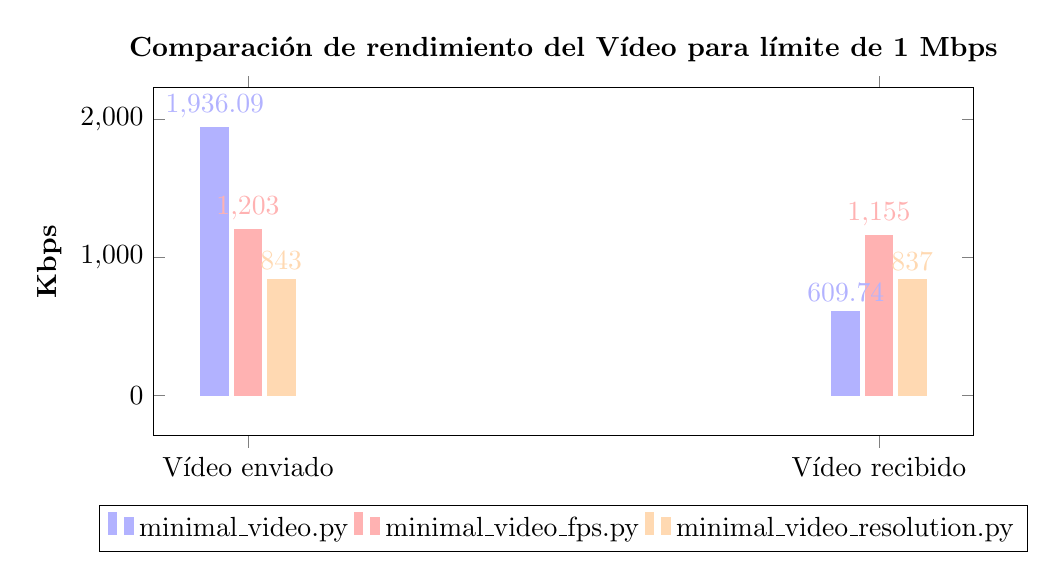
\begin{tikzpicture}
\begin{axis}[
    width=12cm,
    height=6cm,
    ybar,
    enlargelimits=0.15,
    ylabel={\textbf{Kbps}},
    title={\textbf{Comparación de rendimiento del Vídeo para límite de 1 Mbps}},
    symbolic x coords={Vídeo enviado, Vídeo recibido},
    xtick=data,
    nodes near coords,
    nodes near coords align={vertical},
    ymin=0,
    legend style={at={(0.5,-0.2)}, anchor=north, legend columns=3},
    ]
\addplot[blue!30,fill=blue!30] coordinates {(Vídeo enviado, 1936.09) (Vídeo recibido, 609.74)};
\addplot[red!30,fill=red!30] coordinates {(Vídeo enviado, 1203) (Vídeo recibido, 1155)};
\addplot[orange!30,fill=orange!30] coordinates {(Vídeo enviado, 843) (Vídeo recibido, 837)};
\legend{minimal\_video.py, minimal\_video\_fps.py, minimal\_video\_resolution.py}
\end{axis}
\end{tikzpicture}

\vspace{1cm} % Espacio entre gráficas

% Segunda gráfica para Audio con 1 Mbps
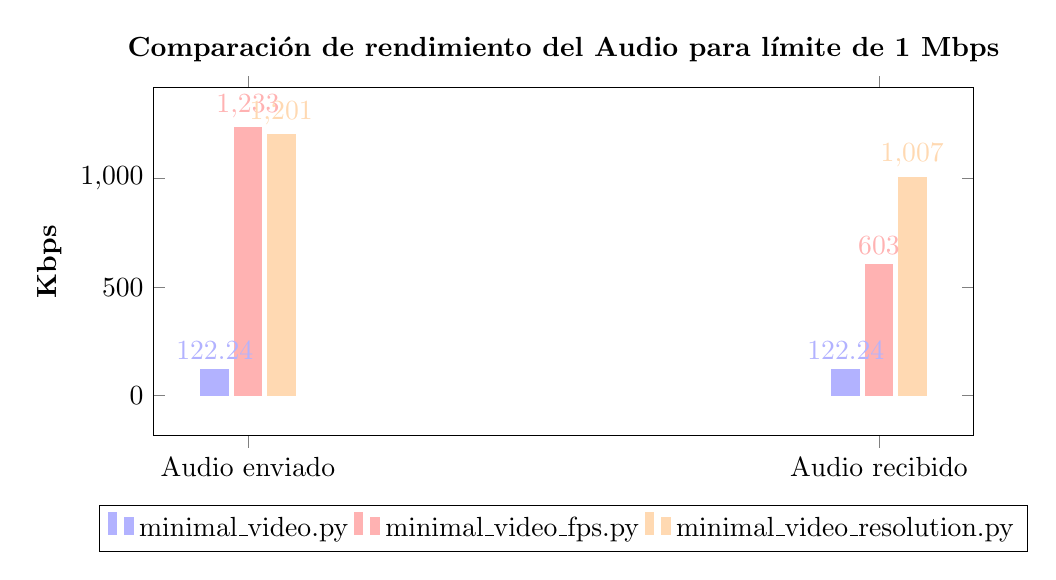
\begin{tikzpicture}
\begin{axis}[
    width=12cm,
    height=6cm,
    ybar,
    enlargelimits=0.15,
    ylabel={\textbf{Kbps}},
    title={\textbf{Comparación de rendimiento del Audio para límite de 1 Mbps}},
    symbolic x coords={Audio enviado, Audio recibido},
    xtick=data,
    nodes near coords,
    nodes near coords align={vertical},
    ymin=0,
    legend style={at={(0.5,-0.2)}, anchor=north, legend columns=3},
    ]
\addplot[blue!30,fill=blue!30] coordinates {(Audio enviado, 122.24) (Audio recibido, 122.24)};
\addplot[red!30,fill=red!30] coordinates {(Audio enviado, 1233) (Audio recibido, 603)};
\addplot[orange!30,fill=orange!30] coordinates {(Audio enviado, 1201) (Audio recibido, 1007)};
\legend{minimal\_video.py, minimal\_video\_fps.py, minimal\_video\_resolution.py}
\end{axis}
\end{tikzpicture}
\caption{Comparación del rendimiento de los tres programas con limitación de 1 Mbps}
\label{fig:comparacion1mbps}
\end{figure}

\vspace{\baselineskip}

Además, a continuación se muestra la eficiencia de FPS en minimal\_video\_fps y minimal\_video\_resolution en el siguiente gráfico:

\begin{figure}[H]
\centering
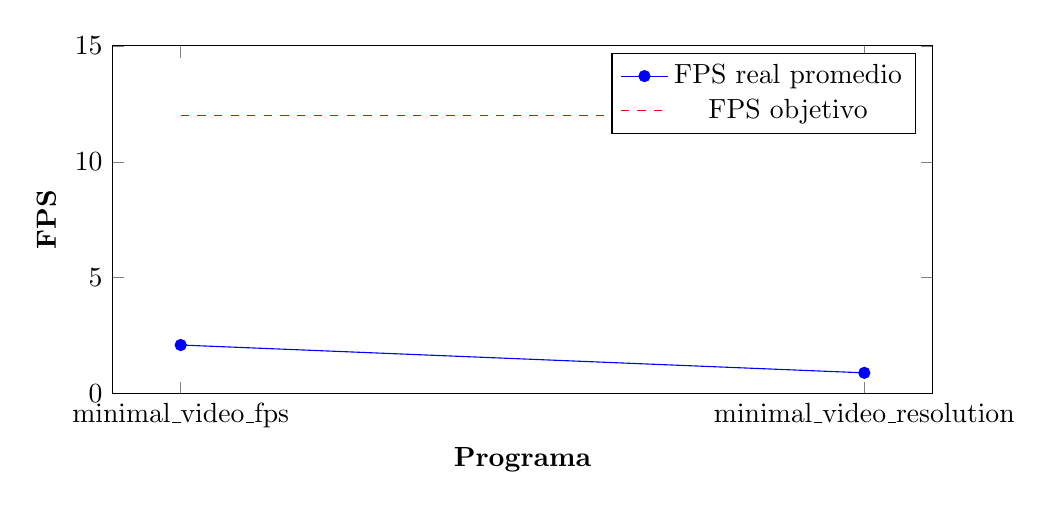
\begin{tikzpicture}
\begin{axis}[
    width=12cm,
    height=6cm,
    xlabel={\textbf{Programa}},
    ylabel={\textbf{FPS}},
    symbolic x coords={minimal\_video\_fps, minimal\_video\_resolution},
    xtick=data,
    ymin=0, 
    ymax=15,
    ]
\addplot[mark=*,blue] coordinates {(minimal\_video\_fps, 2.1) (minimal\_video\_resolution, 0.9)};
\addplot[red,sharp plot,dashed] coordinates {(minimal\_video\_fps, 12) (minimal\_video\_resolution, 12)};
\legend{FPS real promedio, FPS objetivo}
\end{axis}
\end{tikzpicture}
\caption{Comparación de FPS entre los dos programas con limitación de 1 Mbps}
\label{fig:comparacionfps_1mb}
\end{figure}

\textbf{Conclusiones para limitación 1 Mbps:}

En general, estas pruebas demuestran que este ancho de banda es insuficiente para una comunicación de vídeo y audio mínimamente aceptable.
\begin{itemize}
    \item \textbf{Congestión alta:} Todos los módulos intentan enviar muchos más datos de los que la red puede manejar, resultando en que se muestren mensajes de ``Socket bloqueado'' y una pérdida masiva de paquetes.
    \item \textbf{Inficacia de los FPS y el reescalado:} Características como el control de FPS o el reescalado de resolución tuvieron el peor rendimiento en cuanto a datos recibidos.
\end{itemize}

\newpage

\begin{itemize}
  \item \textbf{Prueba de ancho de banda de 10 Mbps:}
\end{itemize}

En esta sección, se analiza el rendimiento de los módulos \texttt{minimal\_video.py}, \texttt{minimal\_video\_fps.py} y \texttt{minimal\_video\_resolution.py} cuando la red se encuentra limitada a un ancho de banda de 10 Mbps. Esta condición representa un entorno más realista respecto a la prueba previa, similar a una conexión doméstica estándar pero con una pobre conexión.
\vspace{\baselineskip}

\textbf{- Análisis de \texttt{minimal\_video.py} con 10 Mbps:}
\vspace{\baselineskip}

El comportamiento de \texttt{minimal\_video.py} bajo el límite del ancho de banda de 10 Mbps mejora notablemente respecto a la prueba de 1 Mbps. Según las estadísticas globales, el módulo intentó enviar 5204 kbps de vídeo y 975 kbps de audio, logrando recibir 4777 kbps de vídeo y 925 kbps de audio. Esto indica que la mayor parte de los datos logra transmitirse correctamente, y la experiencia del usuario es considerablemente mejor: el vídeo y el audio son reconocibles y, en general, funciona.
\vspace{\baselineskip}

Sin embargo, la presencia constante de mensajes como ``Socket bloqueado al enviar fragmento X'' indica que el programa, sigue generando picos de tráfico o un flujo sostenido que en ocasiones excede la capacidad de la red. En ese momento, el socket bloquea temporalmente el envío de nuevos paquetes hasta aliviar la congestión en la cola de red. Esto produce cortes y congelaciones puntuales. El sistema funciona, pero la fluidez no es óptima y aún existen limitaciones claras para un uso completamente estable.

\vspace{\baselineskip}

\textbf{Análisis de \texttt{minimal\_video\_fps.py} con 10 Mbps:}
\vspace{\baselineskip}

Al aumentar el ancho de banda a 10 Mbps, este módulo, que intenta fijar la tasa de FPS en 12, también se experimenta una mejora importante. Las estadísticas muestran que 4853 kbps de vídeo son enviados (4415 kbps recibidos) y 867 kbps de audio son enviados (759 kbps recibidos), datos muy similares al módulo anterior, lo que tiene sentido dado que la única diferencia es la gestión de la tasa de fotogramas.
\vspace{\baselineskip}

Sin embargo, la sección de ``Estadísticas de FPS'' revela que, pese a tener de objetivo 12 FPS, solo se logra un promedio real de 2.8 FPS (eficiencia del 23.5\%). Los mensajes de ``Socket bloqueado'' confirman que, aunque la red permite transmitir una cantidad mayor de datos, todavía es insuficiente para mantener de forma fluida la tasa objetivo con la calidad y resolución establecidas. El control de FPS reduce la carga media, pero los pocos fotogramas que se logran enviar siguen teniendo un tamaño demasiado grande para poder enviarse con un ancho de banda de 10 Mbps sin pérdidas o retrasos. La experiencia es aceptable, pero lejos de lo óptimo para vídeo en tiempo real.

\vspace{\baselineskip}

\textbf{Análisis de \texttt{minimal\_video\_resolution.py} con 10 Mbps:}
\vspace{\baselineskip}

En este caso, el módulo intenta transmitir vídeo a 12 FPS y una resolución objetivo de 350x250 píxeles (ajustando realmente a 352x288 que es la resolución compatible según la cámara). Los datos globales muestran que 5478 kbps de vídeo son enviados (5153 kbps recibidos) y 841 kbps de audio, este último son recibidos en su totalidad.
\vspace{\baselineskip}

Las ``Estadísticas de FPS'' son prácticamente idénticas al módulo anterior: 2.8 FPS reales frente al objetivo de 12 (eficiencia del 23.4\%). Esto confirma que la limitación principal sigue siendo la capacidad de la red. Además, el tiempo de reescalado promedio es de 13.39 ms, con un impacto en CPU del 16.1\%; a diferencia del escenario de 1 Mbps, aquí este consumo resulta importante. Aunque en la salida de este módulo no aparecen explícitamente los mensajes de ``Socket bloqueado'', la baja eficiencia de FPS evidencia que el enlace no puede manejar el volumen de datos necesario para los 12 FPS. El sistema transmite lo que puede, pero está lejos de lograr una experiencia fluida y estable.

\vspace{\baselineskip}

\begin{figure}[H]
\centering
% Primera gráfica para Video con 10 Mbps
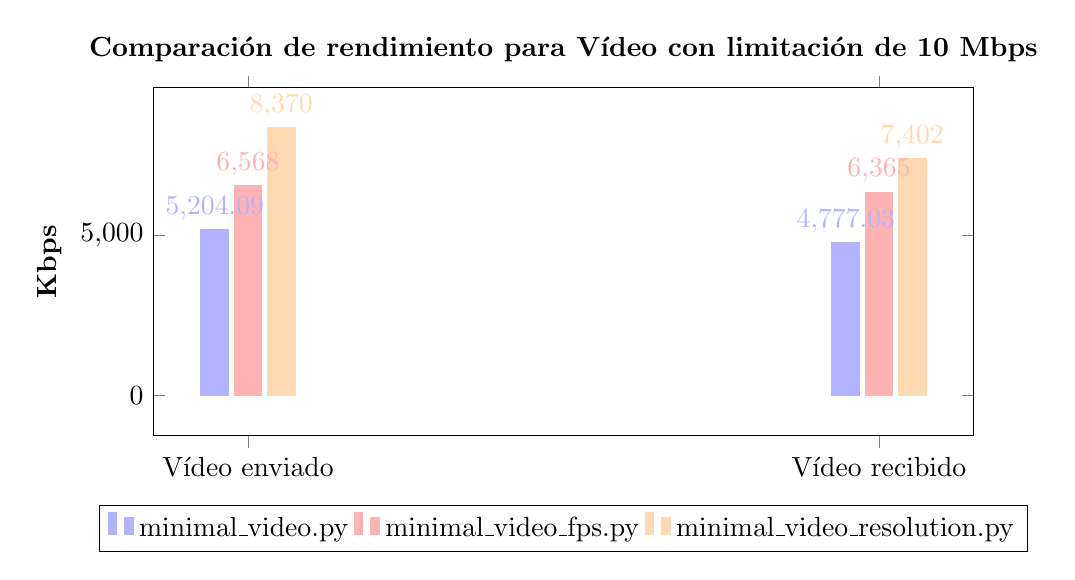
\begin{tikzpicture}
\begin{axis}[
    width=12cm,
    height=6cm,
    ybar,
    enlargelimits=0.15,
    ylabel={\textbf{Kbps}},
    title={\textbf{Comparación de rendimiento para Vídeo con limitación de 10 Mbps}},
    symbolic x coords={Vídeo enviado, Vídeo recibido},
    xtick=data,
    nodes near coords,
    nodes near coords align={vertical},
    ymin=0,
    legend style={at={(0.5,-0.2)}, anchor=north, legend columns=3},
    ]
\addplot[blue!30,fill=blue!30] coordinates {(Vídeo enviado, 5204.09) (Vídeo recibido, 4777.03)};
\addplot[red!30,fill=red!30] coordinates {(Vídeo enviado, 6568) (Vídeo recibido, 6365)};
\addplot[orange!30,fill=orange!30] coordinates {(Vídeo enviado, 8370) (Vídeo recibido, 7402)};
\legend{minimal\_video.py, minimal\_video\_fps.py, minimal\_video\_resolution.py}
\end{axis}
\end{tikzpicture}

\vspace{1cm} % Espacio entre gráficas

% Segunda gráfica para Audio con 10 Mbps
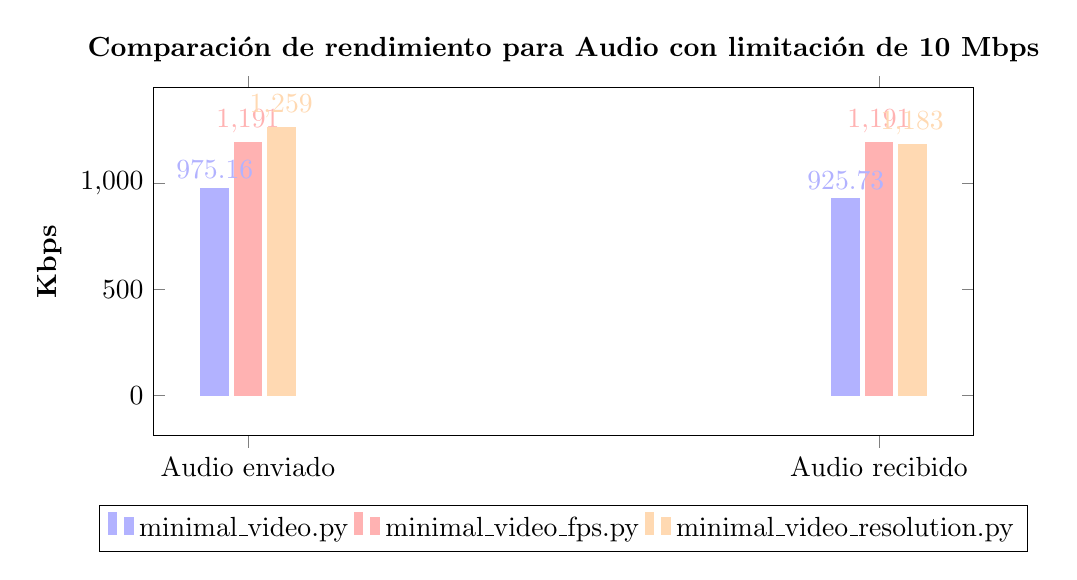
\begin{tikzpicture}
\begin{axis}[
    width=12cm,
    height=6cm,
    ybar,
    enlargelimits=0.15,
    ylabel={\textbf{Kbps}},
    title={\textbf{Comparación de rendimiento para Audio con limitación de 10 Mbps}},
    symbolic x coords={Audio enviado, Audio recibido},
    xtick=data,
    nodes near coords,
    nodes near coords align={vertical},
    ymin=0,
    legend style={at={(0.5,-0.2)}, anchor=north, legend columns=3},
    ]
\addplot[blue!30,fill=blue!30] coordinates {(Audio enviado, 975.16) (Audio recibido, 925.73)};
\addplot[red!30,fill=red!30] coordinates {(Audio enviado, 1191) (Audio recibido, 1191)};
\addplot[orange!30,fill=orange!30] coordinates {(Audio enviado, 1259) (Audio recibido, 1183)};
\legend{minimal\_video.py, minimal\_video\_fps.py, minimal\_video\_resolution.py}
\end{axis}
\end{tikzpicture}
\caption{Comparación del rendimiento de los tres programas con limitación de 10 Mbps}
\label{fig:comparacion10mbps}
\end{figure}

\vspace{\baselineskip}

Además, a continuación se muestra la eficiencia de FPS en minimal\_video\_fps y minimal\_video\_resolution en el siguiente gráfico:
\begin{figure}[H]
\centering
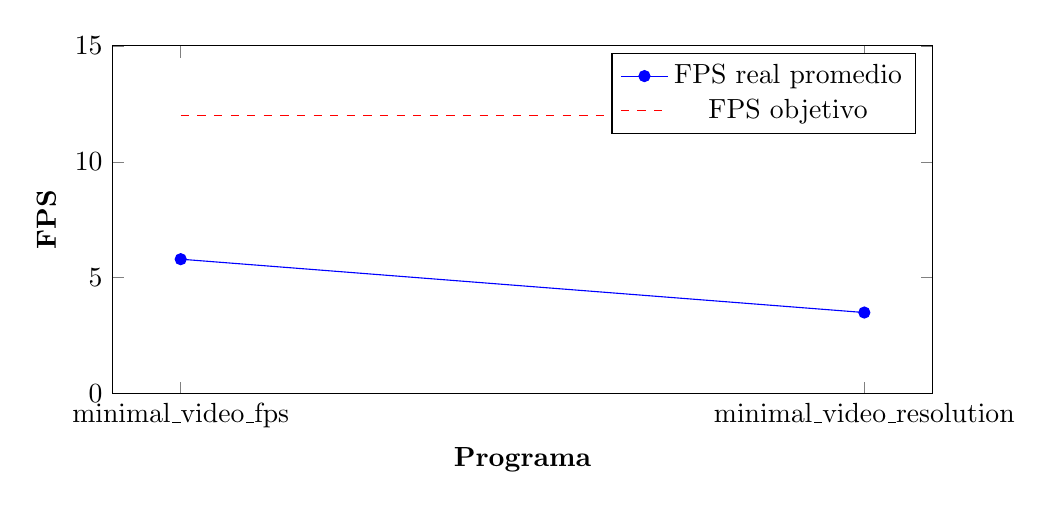
\begin{tikzpicture}
\begin{axis}[
    width=12cm,
    height=6cm,
    xlabel={\textbf{Programa}},
    ylabel={\textbf{FPS}},
    symbolic x coords={minimal\_video\_fps, minimal\_video\_resolution},
    xtick=data,
    ymin=0, 
    ymax=15,
    ]
\addplot[mark=*,blue] coordinates {(minimal\_video\_fps, 5.8) (minimal\_video\_resolution, 3.5)};
\addplot[red,sharp plot,dashed] coordinates {(minimal\_video\_fps, 12) (minimal\_video\_resolution, 12)};
\legend{FPS real promedio, FPS objetivo}
\end{axis}
\end{tikzpicture}
\caption{Comparación de FPS entre los dos programas con limitación de 10 Mbps}
\label{fig:comparacionfps_10mb}
\end{figure}

\textbf{Conclusiones para limitación 10 Mbps:}

La ejecución de los programas con un ancho de banda de 10 Mbps supone una mjoera considerable respecto a 1 Mbps, permitiendo una comunicación básica y, en la mayoría de los casos, funcional.
\begin{itemize}
    \item \textbf{Transmisión parcialmente exitosa:} La mayoría de los datos de audio y vídeo logran transmitirse, lo que permite una comunicación reconocible, aunque no de calidad óptima.
    \item \textbf{Congestión persistente:} Los mensajes de ``Socket bloqueado'' y la baja eficiencia de FPS muestran que 10 Mbps sigue siendo insuficiente para soportar el volumen de datos necesario para una experiencia totalmente fluida, sobre todo en vídeo con 12 FPS.
    \item \textbf{Impacto de funciones avanzadas:} El control de FPS y el reescalado de resolución funcionan técnicamente, pero su uso se ve limitado por el cuello de botella de la red; además, el coste de CPU del reescalado empieza a ser relativamente considerable.
    \item \textbf{Comportamiento mejorado, pero limitado:} Aunque el sistema es usable y la transmisión mejora, aún no se logra una experiencia de videollamada fluida. Para conseguirlo, sería necesario un mayor ancho de banda.
\end{itemize}


\newpage

\begin{itemize}
  \item \textbf{Prueba de ancho de banda de 50 Mbps:}
\end{itemize}

Continuamos nuestro análisis de los tres módulos \texttt{minimal\_video.py}, \texttt{minimal\_video\_fps.py} y \texttt{minimal\_video\_resolution.py} cuando la red se limita a un ancho de banda de 50 Mbps. Esta condición representa un entorno de conexión considerablemente mejor, similar a una conexión de fibra óptica doméstica básica o una buena conexión ADSL.

\vspace{\baselineskip}

\textbf{- Análisis de \texttt{minimal\_video.py} con 50 Mbps:}
\vspace{\baselineskip}

Al examinar el comportamiento de \texttt{minimal\_video.py} bajo esta condición, se observa una mejora drástica respecto a las pruebas anteriores. Las estadísticas globales muestran que el módulo intentó enviar 6967.88 kbps de vídeo y 1037.56 kbps de audio, logrando recibir 6358.18 kbps y 965.31 kbps respectivamente. Estos valores representan un porcentaje de recepción muy alto (más del 90\% de los datos enviados), lo que indica que se aprovecha el ancho de banda disponible.
\vspace{\baselineskip}

Al contrario que las pruebas anteriores, los mensajes de ``Socket bloqueado'' prácticamente desaparecen, lo que confirma que la red puede manejar adecuadamente el flujo de datos generado por el programa. La experiencia del usuario mejora notablemente: el vídeo se muestra fluido y el audio se escucha claro y continuo. Sin embargo, dado que el programa no implementa un control específico de FPS, la tasa de fotogramas puede variar según las condiciones del sistema, alcanzando aproximadamente unos 8 FPS en promedio.

\vspace{\baselineskip}

\textbf{Análisis de \texttt{minimal\_video\_fps.py} con 50 Mbps:}
\vspace{\baselineskip}

Este módulo, intenta obtener una tasa de fotogramas a 12 FPS, muestra un comportamiento interesante bajo esta condición de red. Los datos muestran un envío de 7226.78 kbps de vídeo (6363.69 kbps recibidos) y 905.71 kbps de audio (769.17 kbps recibidos). El porcentaje de recepción es bastante alto, aunque menor de lo que cabría esperar con un ancho de banda de 50 Mbps, lo que sugiere que podrían existir otros factores limitantes además de la red.
\vspace{\baselineskip}

La parte de ``Estadísticas de FPS'' revela un resultado menos óptimo de lo esperado: el programa alcanza aproximadamente 4.4 FPS reales frente al objetivo de 12 FPS, lo que representa una eficiencia del 37.0\%. Aunque esto supone una mejora respecto a las pruebas con anchos de banda más limitados, está lejos de ser ideal. Este rendimiento sugiere que, incluso con un ancho de banda suficiente, existen otras limitaciones (posiblemente relacionadas con el hardware, el procesamiento o la implementación del control de FPS) que impiden alcanzar la tasa objetivo. A pesar de esto, la experiencia del usuario sería notablemente mejor que en las pruebas con anchos de banda menores, con un vídeo más fluido y predecible.

\vspace{\baselineskip}

\textbf{Análisis de \texttt{minimal\_video\_resolution.py} con 50 Mbps:}
\vspace{\baselineskip}

Este módulo, que combina el control de FPS con una resolución configurada para 350x250, muestra un comportamiento interesante bajo las condiciones de 50 Mbps. Las estadísticas globales indican un envío de 8140.48 kbps de vídeo (7780.03 kbps recibidos) y 875.60 kbps de audio (833.37 kbps recibidos). El alto porcentaje de recepción confirma que el ancho de banda es suficiente para esta versión del programa.

Las ``Estadísticas de FPS'' muestran que se logran 5.2 FPS reales de los 12 FPS objetivo (eficiencia del 43.4\%). Aunque inferior al rendimiento esperado, sigue siendo mejor que en pruebas con anchos de banda más limitados. El ``Tiempo de reescalado promedio'' es de 3.92 ms, con un impacto en el rendimiento (CPU) del 4.7\%. Este coste de procesamiento es relativamente bajo, lo que permite una experiencia de usuario equilibrada entre calidad de imagen y fluidez.

La resolución real utilizada es 352x288 (la más cercana compatible con la cámara), lo que explica el volumen de datos enviados.

\vspace{\baselineskip}

\begin{figure}[H]
\centering
% Primera gráfica para Video con 50 Mbps
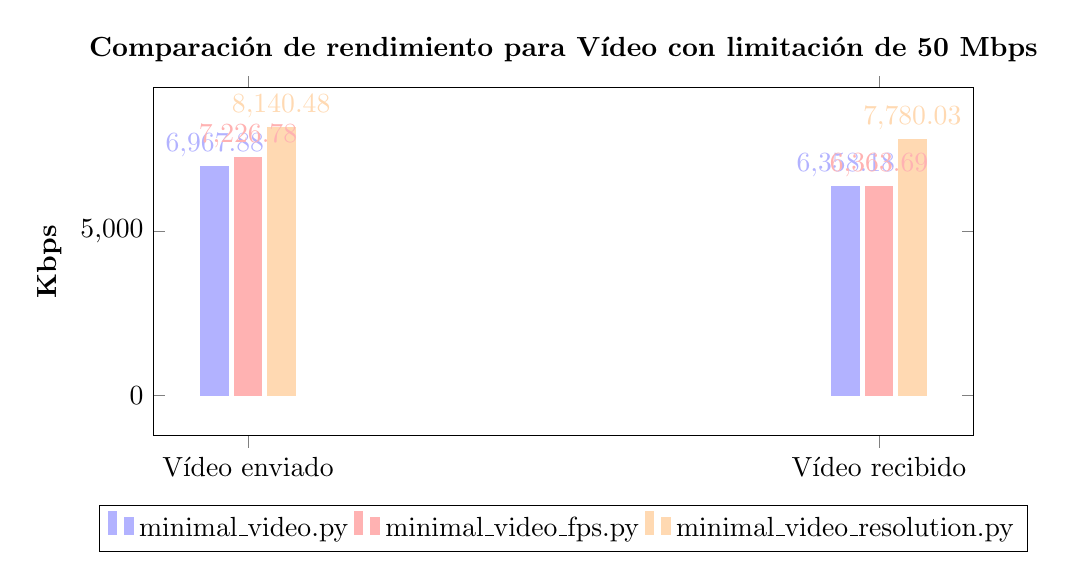
\begin{tikzpicture}
\begin{axis}[
    width=12cm,
    height=6cm,
    ybar,
    enlargelimits=0.15,
    ylabel={\textbf{Kbps}},
    title={\textbf{Comparación de rendimiento para Vídeo con limitación de 50 Mbps}},
    symbolic x coords={Vídeo enviado, Vídeo recibido},
    xtick=data,
    nodes near coords,
    nodes near coords align={vertical},
    ymin=0,
    legend style={at={(0.5,-0.2)}, anchor=north, legend columns=3},
    ]
\addplot[blue!30,fill=blue!30] coordinates {(Vídeo enviado, 6967.88) (Vídeo recibido, 6358.18)};
\addplot[red!30,fill=red!30] coordinates {(Vídeo enviado, 7226.78) (Vídeo recibido, 6363.69)};
\addplot[orange!30,fill=orange!30] coordinates {(Vídeo enviado, 8140.48) (Vídeo recibido, 7780.03)};
\legend{minimal\_video.py, minimal\_video\_fps.py, minimal\_video\_resolution.py}
\end{axis}
\end{tikzpicture}

\vspace{1cm} % Espacio entre gráficas

% Segunda gráfica para Audio con 50 Mbps
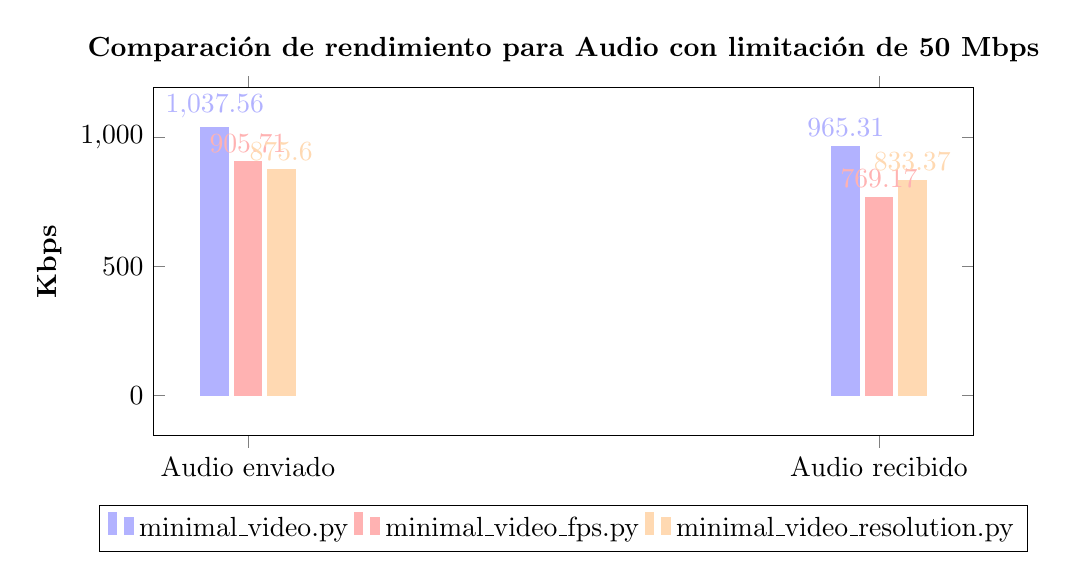
\begin{tikzpicture}
\begin{axis}[
    width=12cm,
    height=6cm,
    ybar,
    enlargelimits=0.15,
    ylabel={\textbf{Kbps}},
    title={\textbf{Comparación de rendimiento para Audio con limitación de 50 Mbps}},
    symbolic x coords={Audio enviado, Audio recibido},
    xtick=data,
    nodes near coords,
    nodes near coords align={vertical},
    ymin=0,
    legend style={at={(0.5,-0.2)}, anchor=north, legend columns=3},
    ]
\addplot[blue!30,fill=blue!30] coordinates {(Audio enviado, 1037.56) (Audio recibido, 965.31)};
\addplot[red!30,fill=red!30] coordinates {(Audio enviado, 905.71) (Audio recibido, 769.17)};
\addplot[orange!30,fill=orange!30] coordinates {(Audio enviado, 875.60) (Audio recibido, 833.37)};
\legend{minimal\_video.py, minimal\_video\_fps.py, minimal\_video\_resolution.py}
\end{axis}
\end{tikzpicture}
\caption{Comparación del rendimiento de los tres programas con limitación de 50 Mbps}
\label{fig:comparacion50mbps}
\end{figure}

\vspace{\baselineskip}

Además, a continuación se muestra la eficiencia de FPS en minimal\_video\_fps y minimal\_video\_resolution en el siguiente gráfico:
\begin{figure}[H]
\centering
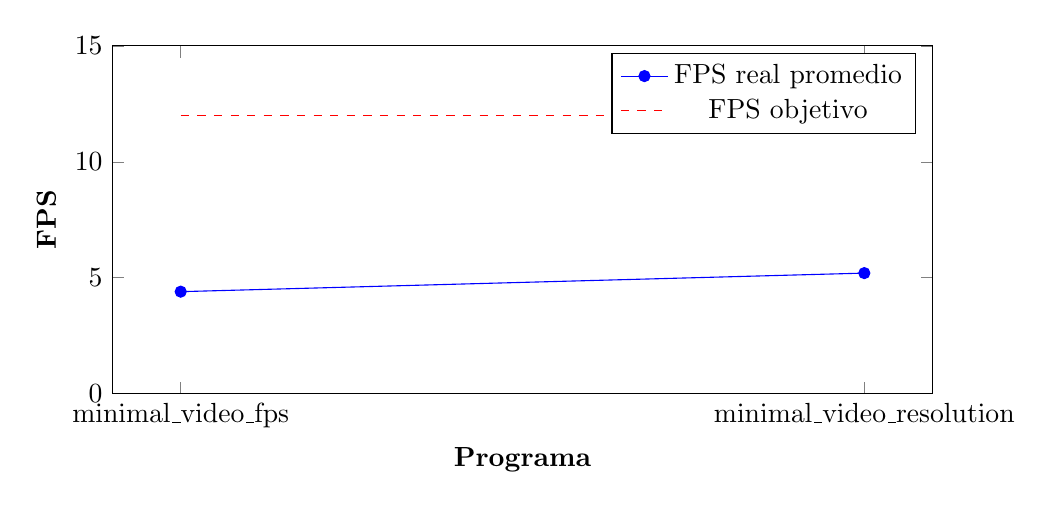
\begin{tikzpicture}
\begin{axis}[
    width=12cm,
    height=6cm,
    xlabel={\textbf{Programa}},
    ylabel={\textbf{FPS}},
    symbolic x coords={minimal\_video\_fps, minimal\_video\_resolution},
    xtick=data,
    ymin=0, 
    ymax=15,
    ]
\addplot[mark=*,blue] coordinates {(minimal\_video\_fps, 4.4) (minimal\_video\_resolution, 5.2)};
\addplot[red,sharp plot,dashed] coordinates {(minimal\_video\_fps, 12) (minimal\_video\_resolution, 12)};
\legend{FPS real promedio, FPS objetivo}
\end{axis}
\end{tikzpicture}
\caption{Comparación de FPS entre los dos programas con limitación de 50 Mbps}
\label{fig:comparacionfps_50mb}
\end{figure}

\textbf{Conclusiones para limitación 50 Mbps:}

La ejecución de los programas con un ancho de banda de 50 Mbps muestra un rendimiento significativamente superior, acercándose a una experiencia realmente buena.
\begin{itemize}
    \item \textbf{Transmisión altamente exitosa:} La gran mayoría de los datos enviados son recibidos correctamente, reduciendo notablemente los problemas de pérdida de paquetes y congestión observados en las pruebas anteriores.
    \item \textbf{Ausencia de congestión:} Los mensajes de ``Socket bloqueado'' prácticamente desaparecen, indicando que la red puede manejar adecuadamente el flujo de datos generado por los programas.
    \item \textbf{Eficacia moderada del control de FPS:} El módulo \texttt{minimal\_video\_fps.py} alcanza una eficiencia del 37.0\%, que aunque no es óptima, representa una mejora respecto a anchos de banda menores, sugiriendo que existen otros factores limitantes además de la red.
    \item \textbf{Viabilidad del reescalado de resolución:} Con 50 Mbps, el reescalado a resoluciones como 352x288 se vuelve viable, con un impacto en CPU relativamente bajo (4.7\%) y un rendimiento de FPS similar al del módulo de control de fotogramas.
    \item \textbf{Rendimiento comparable entre módulos:} Curiosamente, el módulo \texttt{minimal\_video\_resolution.py} logra una eficiencia de FPS (43.4\%) ligeramente superior a la del módulo \texttt{minimal\_video\_fps.py} (37.0\%), posiblemente debido a optimizaciones específicas o diferencias en la implementación.
\end{itemize}

Esta prueba demuestra que un ancho de banda de 50 Mbps es suficiente para una experiencia de videollamada de calidad, aunque persisten limitaciones que probablemente estén más relacionadas con el hardware y el procesamiento que con la capacidad de la red.

\newpage

\subsubsection{Pruebas con límite de latencia (Delay)}

\begin{itemize}
  \item \textbf{Prueba de latencia de 0ms:}
\end{itemize}

Continuando con nuestro análisis de las diferentes condiciones de red, examinamos ahora el comportamiento de los tres módulos en una situación ideal de latencia cero (0ms), lo que simula una comunicación en una red local sin retrasos significativos.

\vspace{\baselineskip}

\textbf{- Análisis de \texttt{minimal\_video.py} con 0ms de latencia:}
\vspace{\baselineskip}

Al observar el comportamiento de \texttt{minimal\_video.py} bajo condiciones de latencia cero, se aprecia una transmisión estable y fluida. Las estadísticas globales muestran que el módulo envía audio a una tasa de 1155.34 kbps (recibiendo 1013.26 kbps) y vídeo a 7141.31 kbps (recibiendo 6491.44 kbps). Esto significa en un porcentaje de recepción aproximado del 88-91\%, indicando una transmisión eficiente con muy pocas pérdidas.
\vspace{\baselineskip}

La ausencia de latencia permite que los ciclos de envío y recepción estén bien sincronizados, como se observa en las estadísticas por ciclo, donde se mantiene un flujo constante de mensajes (entre 20-30 mensajes de audio y vídeo por ciclo). El uso de CPU oscila entre un 20-40\% para el programa y 70-79\% para el sistema, lo que indica un procesamiento eficiente sin sobrecarga excesiva. La experiencia de usuario resultante es notablemente mejor que en escenarios con limitaciones de ancho de banda o latencia añadida.

\vspace{\baselineskip}

\textbf{Análisis de \texttt{minimal\_video\_fps.py} con 0ms de latencia:}
\vspace{\baselineskip}

Para este módulo, las estadísticas globales muestran una transmisión de audio de 1075.88 kbps (recibiendo 859.78 kbps) y de vídeo de 6748.03 kbps (recibiendo 6038.40 kbps). Estos valores representan un porcentaje de recepción del 80-89\%, ligeramente inferior al módulo base.
\vspace{\baselineskip}

Lo más relevante son las ``Estadísticas de FPS'', que muestran un promedio real de 3.9 FPS frente al objetivo de 12 FPS, resultando en una eficiencia del 32.5\%. Este dato es sorprendente, pues se espera un mejor rendimiento en condiciones ideales de latencia. Esto sugiere que existen otras limitaciones significativas más allá de la red, probablemente relacionadas con el procesamiento del vídeo o la implementación del control de FPS. Aunque el rendimiento está lejos del objetivo, sigue siendo mejor que en escenarios con restricciones de red más severas.

\vspace{\baselineskip}

\textbf{Análisis de \texttt{minimal\_video\_resolution.py} con 0ms de latencia:}
\vspace{\baselineskip}

Este módulo, combinando control de FPS y resolución reescalada a 352x288, muestra un comportamiento ligeramente superior al anterior bajo condiciones de latencia cero. Los datos globales indican una transmisión de audio de 1076.07 kbps (recibiendo 1039.14 kbps) y de vídeo de 8048.59 kbps (recibiendo 7602.30 kbps), con un porcentaje de recepción del 94-96\%, el más alto de los tres módulos.
\vspace{\baselineskip}

Las ``Estadísticas de FPS'' revelan un promedio de 4.5 FPS reales frente al objetivo de 12 FPS, alcanzando una eficiencia del 37.6\%. Si bien sigue estando por debajo del objetivo, supera ligeramente al módulo anterior. El ``Tiempo de reescalado promedio'' es de 5.11 ms, con un impacto en rendimiento del 6.1\%, valores razonables que limitantan el rendimiento.

\vspace{\baselineskip}

Además, a continuación se muestra la eficiencia de FPS en minimal\_video\_fps y minimal\_video\_resolution en el siguiente gráfico:
\begin{figure}[H]
\centering
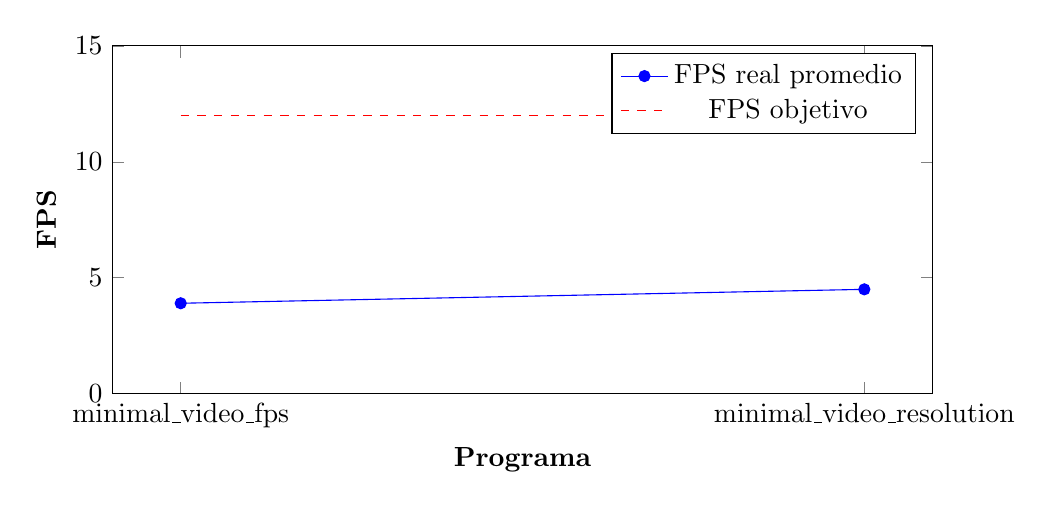
\begin{tikzpicture}
\begin{axis}[
    width=12cm,
    height=6cm,
    xlabel={\textbf{Programa}},
    ylabel={\textbf{FPS}},
    symbolic x coords={minimal\_video\_fps, minimal\_video\_resolution},
    xtick=data,
    ymin=0, 
    ymax=15,
    ]
\addplot[mark=*,blue] coordinates {(minimal\_video\_fps, 3.9) (minimal\_video\_resolution, 4.5)};
\addplot[red,sharp plot,dashed] coordinates {(minimal\_video\_fps, 12) (minimal\_video\_resolution, 12)};
\legend{FPS real promedio, FPS objetivo}
\end{axis}
\end{tikzpicture}
\caption{Comparación de FPS entre los programas con latencia de 0ms}
\label{fig:comparacionfps_0ms}
\end{figure}

También se muestran las tasas de transmisión y recepción de datos en los siguientes gráficos:
\begin{figure}[H]
\centering
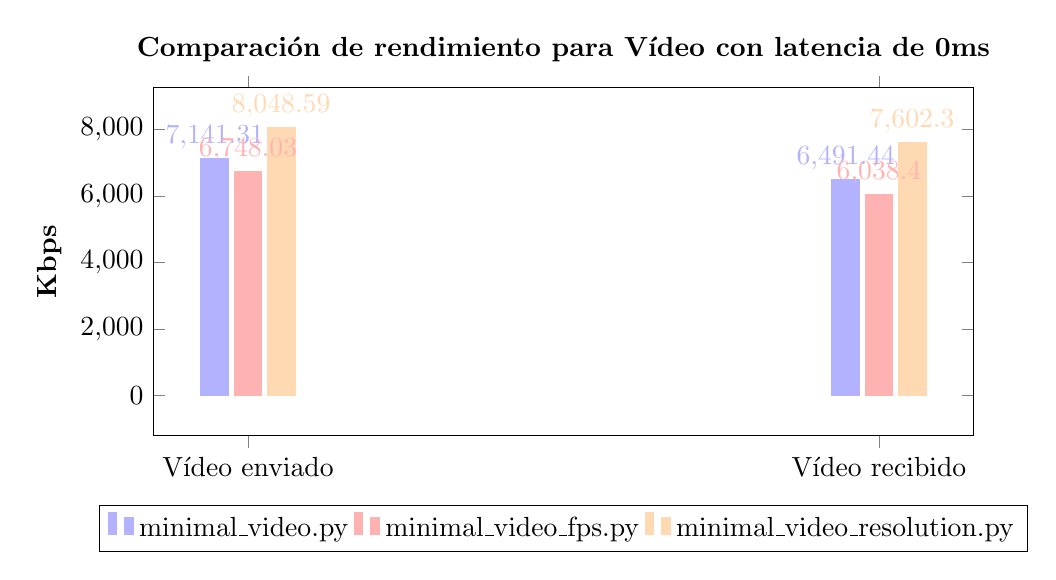
\begin{tikzpicture}
\begin{axis}[
    width=12cm,
    height=6cm,
    ybar,
    enlargelimits=0.15,
    ylabel={\textbf{Kbps}},
    title={\textbf{Comparación de rendimiento para Vídeo con latencia de 0ms}},
    symbolic x coords={Vídeo enviado, Vídeo recibido},
    xtick=data,
    nodes near coords,
    nodes near coords align={vertical},
    ymin=0,
    legend style={at={(0.5,-0.2)}, anchor=north, legend columns=3},
    ]
\addplot[blue!30,fill=blue!30] coordinates {(Vídeo enviado, 7141.31) (Vídeo recibido, 6491.44)};
\addplot[red!30,fill=red!30] coordinates {(Vídeo enviado, 6748.03) (Vídeo recibido, 6038.40)};
\addplot[orange!30,fill=orange!30] coordinates {(Vídeo enviado, 8048.59) (Vídeo recibido, 7602.30)};
\legend{minimal\_video.py, minimal\_video\_fps.py, minimal\_video\_resolution.py}
\end{axis}
\end{tikzpicture}

\vspace{0.8cm} % Espacio entre gráficas

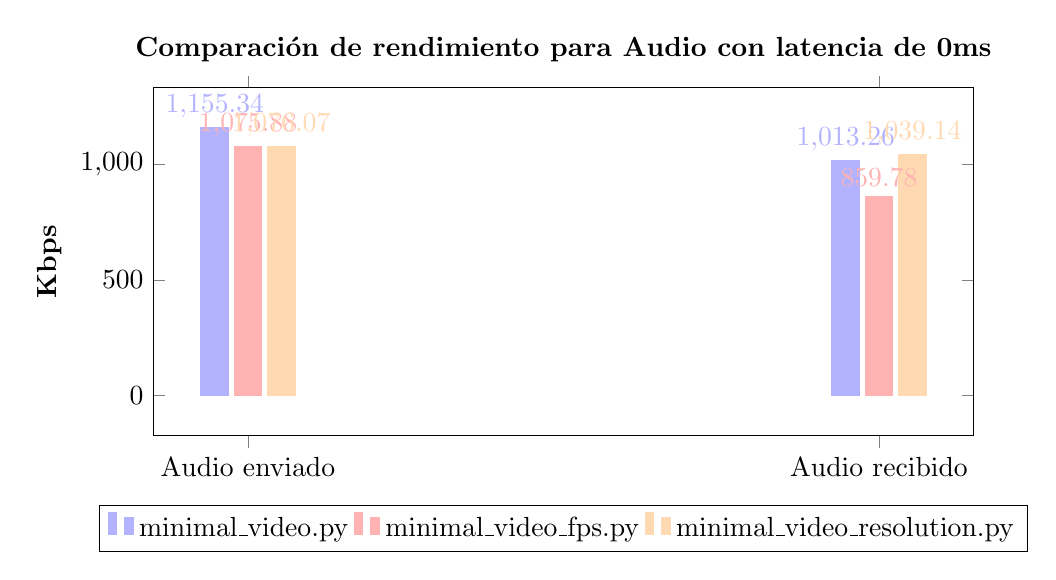
\begin{tikzpicture}
\begin{axis}[
    width=12cm,
    height=6cm,
    ybar,
    enlargelimits=0.15,
    ylabel={\textbf{Kbps}},
    title={\textbf{Comparación de rendimiento para Audio con latencia de 0ms}},
    symbolic x coords={Audio enviado, Audio recibido},
    xtick=data,
    nodes near coords,
    nodes near coords align={vertical},
    ymin=0,
    legend style={at={(0.5,-0.2)}, anchor=north, legend columns=3},
    ]
\addplot[blue!30,fill=blue!30] coordinates {(Audio enviado, 1155.34) (Audio recibido, 1013.26)};
\addplot[red!30,fill=red!30] coordinates {(Audio enviado, 1075.88) (Audio recibido, 859.78)};
\addplot[orange!30,fill=orange!30] coordinates {(Audio enviado, 1076.07) (Audio recibido, 1039.14)};
\legend{minimal\_video.py, minimal\_video\_fps.py, minimal\_video\_resolution.py}
\end{axis}
\end{tikzpicture}
\caption{Comparación del rendimiento de los tres programas con latencia de 0ms}
\label{fig:comparacion0ms}
\end{figure}

\textbf{Conclusiones para latencia 0ms:}

Las pruebas con latencia cero muestran interesaantes resultados en los tres módulos:

\begin{itemize}
    \item \textbf{Transmisión:} Los tres módulos logran tasas de transmisión y recepción relativamente altas, con porcentajes de recepción entre el 80-96\%, siendo \texttt{minimal\_video\_resolution.py} el más eficiente en este aspecto.
    
    \item \textbf{Limitaciones:} Sorprendentemente, incluso en condiciones ideales de latencia, los módulos con control de FPS no logran acercarse a su objetivo de 12 FPS, alcanzando solo entre 3.9-4.5 FPS. Esto sugiere que las limitaciones se encuentran otros componentes del sistema (cámara, procesamiento, implementación del control de FPS).
    
    \item \textbf{Comparación en Rendimiento:} El módulo \texttt{minimal\_video\_resolution.py} muestra un rendimiento ligeramente superior en términos de FPS y porcentaje de recepción de datos, a pesar de transmitir un mayor volumen de información debido al reescalado de la resolución.

  \end{itemize}

Estas pruebas demuestran que, incluso en condiciones ideales de red, existen importantes limitaciones en el rendimiento que probablemente estén relacionadas con otras partes del sistema. Esto sugiere que futuras mejoras deberían enfocarse no solo en la optimización de la transmisión de red, sino también en la optimización del procesamiento del vídeo, la captura de la cámara y la implementación del control de los FPS.

\newpage

\begin{itemize}
  \item \textbf{Prueba de latencia de 100ms:}
\end{itemize}

Seguimos analiazando diferentes condiciones de red, ahora examinaremos el comportamiento de los tres módulos bajo una latencia media de 100ms, que simula una conexión a Internet típica con cierta distancia entre los extremos o con un nivel moderado de congestión.

\vspace{\baselineskip}

\textbf{- Análisis de \texttt{minimal\_video.py} con 100ms de latencia:}
\vspace{\baselineskip}

Al observar el comportamiento de \texttt{minimal\_video.py} bajo una latencia de 100ms, se evidencia un impacto considerable en el rendimiento. Las estadísticas globales muestran que el módulo envía audio a 1179.23 kbps pero recibe solo 636.32 kbps (54\%), mientras que para vídeo envía 8833.52 kbps y recibe 6970.41 kbps (79\%). Esta diferencia entre envío y recepción, especialmente en el audio, indica que la latencia introduce un retraso significativo que afecta la sincronización de la comunicación.
\vspace{\baselineskip}

Un análisis detallado de los ciclos revela un patrón característico: durante los primeros 6-7 ciclos, prácticamente no se recibe ningún paquete, y luego comienza la recepción con valores fluctuantes. Este es el efecto directo del retraso de 100ms, que causa que los primeros paquetes enviados tarden varios ciclos en llegar al receptor. La consecuencia para el usuario es una experiencia menos fluida y desincronización notable entre audio y vídeo.

\vspace{\baselineskip}

\textbf{Análisis de \texttt{minimal\_video\_fps.py} con 100ms de latencia:}
\vspace{\baselineskip}

Para este módulo, que intenta mantener una tasa constante de 12 FPS, la latencia de 100ms tiene un impacto significativo. Las estadísticas globales muestran un envío de audio de 1168.50 kbps (recibiendo 706.70 kbps, 60\%) y de vídeo de 7978.58 kbps (recibiendo 6464.17 kbps, 81\%). Estos porcentajes de recepción, aunque no óptimos, son suficientes para mantener una comunicación aceptable.
\vspace{\baselineskip}

La sección de ``Estadísticas de FPS'' indica que el módulo consigue un promedio de 6.3 FPS reales frente al objetivo de 12 FPS, alcanzando una eficiencia del 52.6\%. Este valor, notablemente mejor que en escenarios con anchos de banda limitados, muestra que el control de FPS consigue adaptarse parcialmente a la latencia actual. El sistema parece ajustar el intervalo entre fotogramas para compensar el retraso, permitiendo una transmisión más sincornizada aunque a costa de una menor fluidez visual. Al igual que en el módulo anterior, se observa un retraso inicial en la recepción de paquetes, seguida por un patrón irregular donde ciclos consecutivos muestran algunas variaciones en la cantidad de datos recibidos.

\vspace{\baselineskip}

\textbf{Análisis de \texttt{minimal\_video\_resolution.py} con 100ms de latencia:}
\vspace{\baselineskip}

Este módulo, combinando control de FPS y resolución reescalada a 352x288, muestra un comportamiento interesante bajo condiciones de latencia de 100ms. Los datos globales indican una transmisión de audio de 1065.15 kbps (recibiendo 916.69 kbps, 86\%) y de vídeo de 10215.56 kbps (recibiendo 9153.09 kbps, 90\%), que son los mejores porcentajes de recepción entre los tres módulos.
\vspace{\baselineskip}

Sin embargo, las ``Estadísticas de FPS'' revelan un promedio de solo 4.2 FPS reales frente al objetivo de 12 FPS, con una eficiencia del 35.0\%. Esta contradicción (mejor tasa de recepción pero peor eficiencia de FPS) sugiere que el módulo prioriza la integridad de los datos enviados sobre la frecuencia de envío. Es decir, envía menos fotogramas pero se asegura de que lleguen completos. El ``Tiempo de reescalado promedio'' es de 5.37 ms, con un impacto en rendimiento del 6.4\%, valores similares a los observados en condiciones sin latencia, lo que indica que esta funcionalidad no se ve afectada por el retraso de la red.

\vspace{\baselineskip}

Además, a continuación se muestra la eficiencia de FPS en minimal\_video\_fps y minimal\_video\_resolution en el siguiente gráfico:
\begin{figure}[H]
\centering
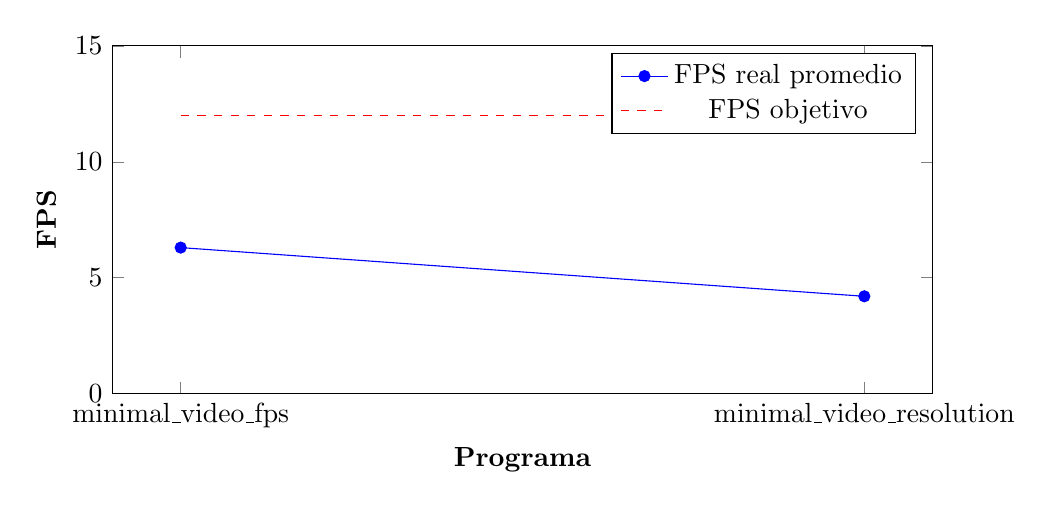
\begin{tikzpicture}
\begin{axis}[
    width=12cm,
    height=6cm,
    xlabel={\textbf{Programa}},
    ylabel={\textbf{FPS}},
    symbolic x coords={minimal\_video\_fps, minimal\_video\_resolution},
    xtick=data,
    ymin=0, 
    ymax=15,
    ]
\addplot[mark=*,blue] coordinates {(minimal\_video\_fps, 6.3) (minimal\_video\_resolution, 4.2)};
\addplot[red,sharp plot,dashed] coordinates {(minimal\_video\_fps, 12) (minimal\_video\_resolution, 12)};
\legend{FPS real promedio, FPS objetivo}
\end{axis}
\end{tikzpicture}
\caption{Comparación de FPS entre los dos programas con latencia de 100ms}
\label{fig:comparacionfps_100ms}
\end{figure}

También se muestran las tasas de transmisión y recepción de datos en los siguientes gráficos:
\begin{figure}[H]
\centering
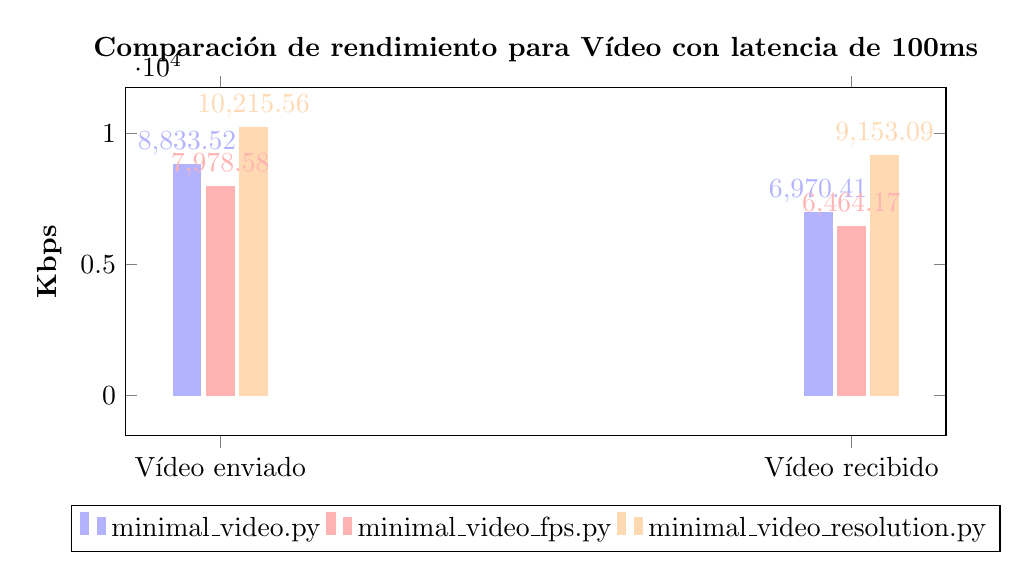
\begin{tikzpicture}
\begin{axis}[
    width=12cm,
    height=6cm,
    ybar,
    enlargelimits=0.15,
    ylabel={\textbf{Kbps}},
    title={\textbf{Comparación de rendimiento para Vídeo con latencia de 100ms}},
    symbolic x coords={Vídeo enviado, Vídeo recibido},
    xtick=data,
    nodes near coords,
    nodes near coords align={vertical},
    ymin=0,
    legend style={at={(0.5,-0.2)}, anchor=north, legend columns=3},
    ]
\addplot[blue!30,fill=blue!30] coordinates {(Vídeo enviado, 8833.52) (Vídeo recibido, 6970.41)};
\addplot[red!30,fill=red!30] coordinates {(Vídeo enviado, 7978.58) (Vídeo recibido, 6464.17)};
\addplot[orange!30,fill=orange!30] coordinates {(Vídeo enviado, 10215.56) (Vídeo recibido, 9153.09)};
\legend{minimal\_video.py, minimal\_video\_fps.py, minimal\_video\_resolution.py}
\end{axis}
\end{tikzpicture}

\vspace{0.5cm} % Espacio entre gráficas

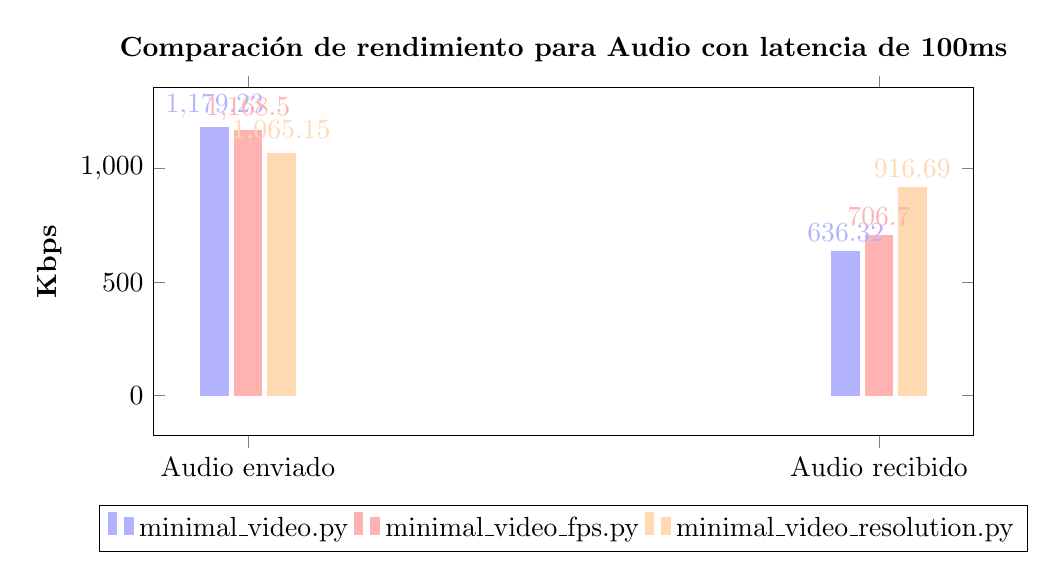
\begin{tikzpicture}
\begin{axis}[
    width=12cm,
    height=6cm,
    ybar,
    enlargelimits=0.15,
    ylabel={\textbf{Kbps}},
    title={\textbf{Comparación de rendimiento para Audio con latencia de 100ms}},
    symbolic x coords={Audio enviado, Audio recibido},
    xtick=data,
    nodes near coords,
    nodes near coords align={vertical},
    ymin=0,
    legend style={at={(0.5,-0.2)}, anchor=north, legend columns=3},
    ]
\addplot[blue!30,fill=blue!30] coordinates {(Audio enviado, 1179.23) (Audio recibido, 636.32)};
\addplot[red!30,fill=red!30] coordinates {(Audio enviado, 1168.50) (Audio recibido, 706.70)};
\addplot[orange!30,fill=orange!30] coordinates {(Audio enviado, 1065.15) (Audio recibido, 916.69)};
\legend{minimal\_video.py, minimal\_video\_fps.py, minimal\_video\_resolution.py}
\end{axis}
\end{tikzpicture}
\caption{Comparación del rendimiento de los tres programas con latencia de 100ms}
\label{fig:comparacion100ms}
\end{figure}

\textbf{Conclusiones para latencia de 100ms:}

La introducción de una latencia de 100ms muestra aspectos interesantes sobre el comportamiento de los tres módulos:

\begin{itemize}
    \item \textbf{Efecto del retardo inicial:} Los tres módulos comienzan de la misma forma, donde los primeros ciclos muestran poca o ninguna recepción, seguidos por un patrón irregular de transmisión que refleja directamente el impacto de la latencia.
    
    \item \textbf{Diferencia entre envío y recepción:} La latencia genera una diferencia significativa entre los datos enviados y recibidos, especialmente notable en el audio para \texttt{minimal\_video.py} (54\%) y \texttt{minimal\_video\_fps.py} (60\%).
    
    \item \textbf{Adaptación:} El módulo \texttt{minimal\_video\_fps.py} muestra la mejor eficiencia de FPS (52.6\%), indicando que logra adaptarse bien a la latencia introducida.
    
    \item \textbf{Prioridades diferentes:} El módulo \texttt{minimal\_video\_resolution.py} presenta los mejores porcentajes de recepción (86-90\%) pero la menor eficiencia de FPS (35.0\%), lo que indica que prioriza la integridad de los datos sobre la frecuencia de fotogramas.
    
    \item \textbf{Impacto asimétrico:} La latencia afecta de manera distinta al audio y al vídeo, con ciclos donde el audio se transmite correctamente mientras el vídeo sufre pérdidas significativas, o viceversa.
\end{itemize}

Estas conclusiones muestran que aunque una latencia de 100ms permite mantener una comunicación funcional, supone sin embargo, limitaciones notables en el rendimiento y lastra la fluidez visual, la calidad de audio y la sincronización entre ambos.

\newpage

\begin{itemize}
  \item \textbf{Prueba de latencia de 250ms:}
\end{itemize}

Finalmente para terminar con las pruebas de latencia, examinamos el comportamiento de los tres módulos bajo una condición de latencia alta de 250ms, que representa una situación de red congestionada o una conexión entre grandes distancias, como podría ser una comunicación intercontinental o una red satelital.

\vspace{\baselineskip}

\textbf{- Análisis de \texttt{minimal\_video.py} con 250ms de latencia:}
\vspace{\baselineskip}

Al analizar el comportamiento de \texttt{minimal\_video.py} bajo esta latencia tan elevada, observamos un impacto considerable. Las estadísticas globales muestran que el módulo envía audio a 1044.97 kbps (recibiendo 824.80 kbps, 79\%) y vídeo a 9296.39 kbps (recibiendo 7781.52 kbps, 84\%). Estos porcentajes de recepción, aunque inferiores a los escenarios con menor latencia, siguen permitiendo una comunicación básica.
\vspace{\baselineskip}

El análisis de los ciclos muestra que inicialmente hay ciclos completos sin recepción de datos, seguidos por ciclos donde se recibe parcialmente y luego se estabiliza. Concretamente en los ciclos 2-7, observamos una recepción muy irregular, que afecta directamente la experiencia del usuario con pausas y cortes. Además, se aprecia que la imagen y el sonido van a tirones, con momentos de congelación.

\vspace{\baselineskip}

\textbf{Análisis de \texttt{minimal\_video\_fps.py} con 250ms de latencia:}
\vspace{\baselineskip}

Este módulo muestra una adaptación interesante a la latencia tan elevada. Las estadísticas globales indican una transmisión de audio de 1127.14 kbps (recibiendo 943.42 kbps, 84\%) y de vídeo de 10848.86 kbps (recibiendo 9626.26 kbps, 89\%). Estos porcentajes son notablemente mejores que para el módulo base, sugiriendo que el control de FPS ayuda a optimizar la transmisión incluso con alta latencia.
\vspace{\baselineskip}

Las ``Estadísticas de FPS'' revelan un dato sorprendentemente positivo. El módulo consigue mantener 7.2 FPS reales frente al objetivo de 12 FPS, alcanzando una eficiencia del 60.1\%. Esto significa que funciona mejor de lo esperado para una latencia tan alta. Ademas indica que el control de FPS consigue adaptarse satisfactoriamente reduciendo la frecuencia de envío de fotogramas para adaptarse a las limitaciones. Sin embargo, la visualización sigue siendo intermitente causando también congelaciones momentáneas en la visualización.

\vspace{\baselineskip}

\textbf{Análisis de \texttt{minimal\_video\_resolution.py} con 250ms de latencia:}
\vspace{\baselineskip}

Los resultados de este módulo bajo una latencia de 250ms son interesantes. Los datos globales muestran una transmisión de audio de 1079.08 kbps (recibiendo 818.01 kbps, 76\%) y de vídeo de 10215.45 kbps (recibiendo 8962.97 kbps, 88\%). Estos porcentajes de recepción son comparables a los del módulo anterior, indicando una buena gestión del flujo de datos a pesar de la resolución reescalada.
\vspace{\baselineskip}

Lo más sorprendente son las ``Estadísticas de FPS'', que revelan un promedio de 9.4 FPS reales frente al objetivo de 12 FPS, alcanzando una eficiencia del 78.0\%. Este resultado, el mejor de los tres módulos, sugiere que la combinación de control de FPS y resolución adaptada a 352x288, es especialmente efectiva para mitigar los efectos de la alta latencia. El ``Tiempo de reescalado promedio'' es de 6.09 ms, con un impacto en rendimiento del 7.3\%, valores ligeramente superiores a los observados en condiciones con menor latencia, pero aún dentro de un rango aceptable.

\vspace{\baselineskip}

Además, a continuación se muestra la eficiencia de FPS en minimal\_video\_fps y minimal\_video\_resolution en el siguiente gráfico:
\begin{figure}[H]
\centering
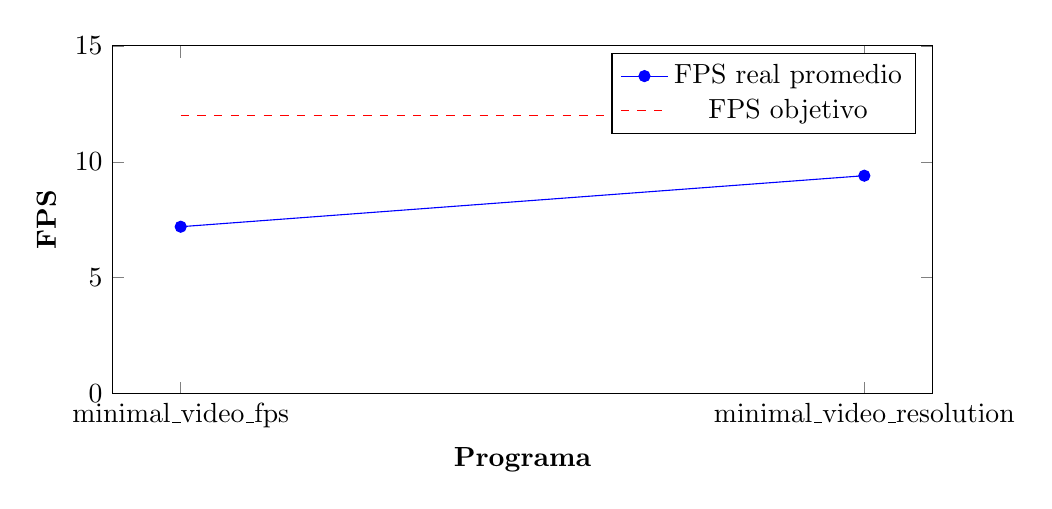
\begin{tikzpicture}
\begin{axis}[
    width=12cm,
    height=6cm,
    xlabel={\textbf{Programa}},
    ylabel={\textbf{FPS}},
    symbolic x coords={minimal\_video\_fps, minimal\_video\_resolution},
    xtick=data,
    ymin=0, 
    ymax=15,
    ]
\addplot[mark=*,blue] coordinates {(minimal\_video\_fps, 7.2) (minimal\_video\_resolution, 9.4)};
\addplot[red,sharp plot,dashed] coordinates {(minimal\_video\_fps, 12) (minimal\_video\_resolution, 12)};
\legend{FPS real promedio, FPS objetivo}
\end{axis}
\end{tikzpicture}
\caption{Comparación de FPS entre los dos programas con latencia de 250ms}
\label{fig:comparacionfps_250ms}
\end{figure}

También se muestran las tasas de transmisión y recepción de datos en los siguientes gráficos:
\begin{figure}[H]
\centering
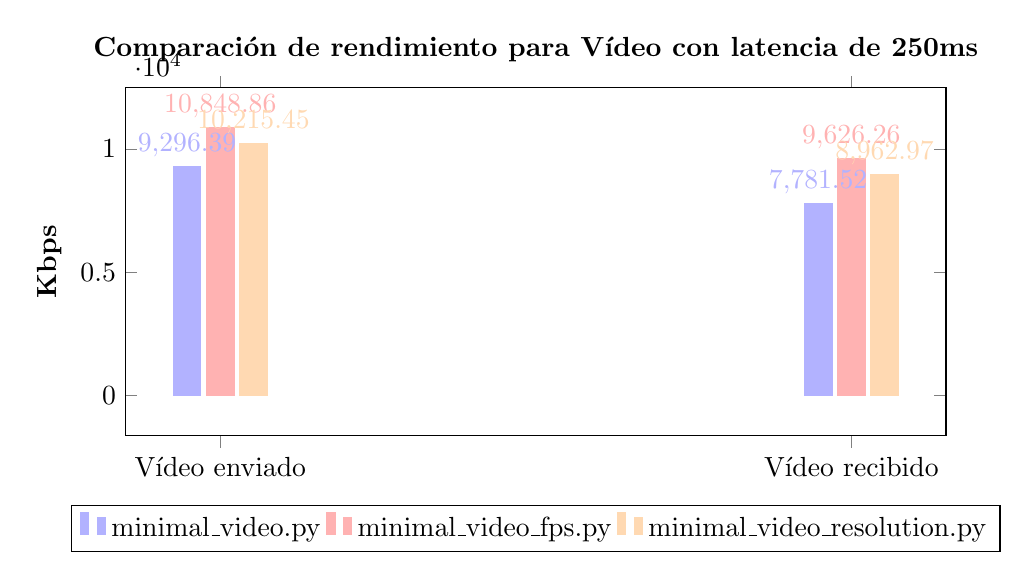
\begin{tikzpicture}
\begin{axis}[
    width=12cm,
    height=6cm,
    ybar,
    enlargelimits=0.15,
    ylabel={\textbf{Kbps}},
    title={\textbf{Comparación de rendimiento para Vídeo con latencia de 250ms}},
    symbolic x coords={Vídeo enviado, Vídeo recibido},
    xtick=data,
    nodes near coords,
    nodes near coords align={vertical},
    ymin=0,
    legend style={at={(0.5,-0.2)}, anchor=north, legend columns=3},
    ]
\addplot[blue!30,fill=blue!30] coordinates {(Vídeo enviado, 9296.39) (Vídeo recibido, 7781.52)};
\addplot[red!30,fill=red!30] coordinates {(Vídeo enviado, 10848.86) (Vídeo recibido, 9626.26)};
\addplot[orange!30,fill=orange!30] coordinates {(Vídeo enviado, 10215.45) (Vídeo recibido, 8962.97)};
\legend{minimal\_video.py, minimal\_video\_fps.py, minimal\_video\_resolution.py}
\end{axis}
\end{tikzpicture}

\vspace{0.5cm} % Espacio entre gráficas

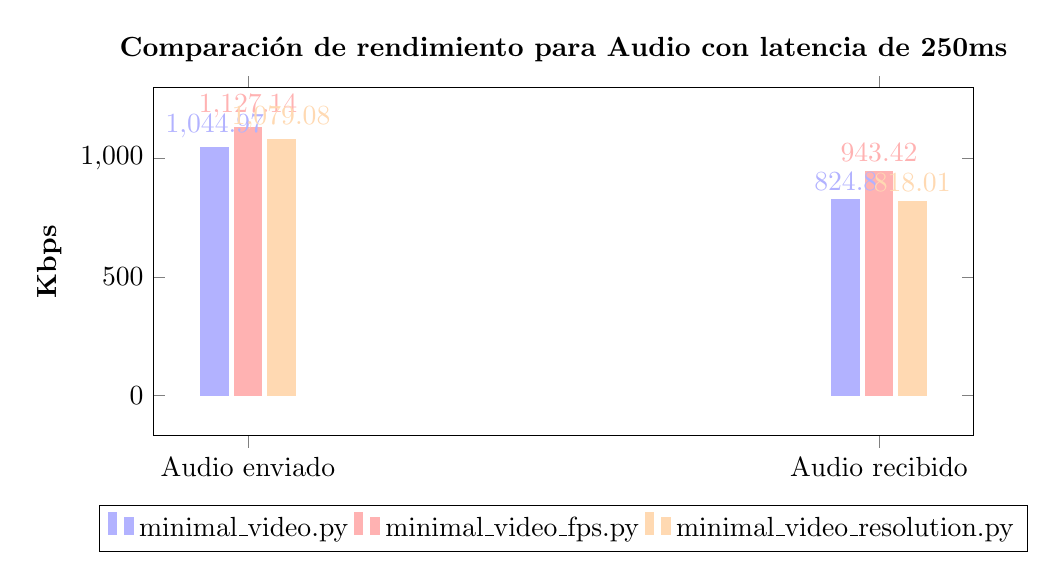
\begin{tikzpicture}
\begin{axis}[
    width=12cm,
    height=6cm,
    ybar,
    enlargelimits=0.15,
    ylabel={\textbf{Kbps}},
    title={\textbf{Comparación de rendimiento para Audio con latencia de 250ms}},
    symbolic x coords={Audio enviado, Audio recibido},
    xtick=data,
    nodes near coords,
    nodes near coords align={vertical},
    ymin=0,
    legend style={at={(0.5,-0.2)}, anchor=north, legend columns=3},
    ]
\addplot[blue!30,fill=blue!30] coordinates {(Audio enviado, 1044.97) (Audio recibido, 824.80)};
\addplot[red!30,fill=red!30] coordinates {(Audio enviado, 1127.14) (Audio recibido, 943.42)};
\addplot[orange!30,fill=orange!30] coordinates {(Audio enviado, 1079.08) (Audio recibido, 818.01)};
\legend{minimal\_video.py, minimal\_video\_fps.py, minimal\_video\_resolution.py}
\end{axis}
\end{tikzpicture}
\caption{Comparación del rendimiento de los tres programas con latencia de 250ms}
\label{fig:comparacion250ms}
\end{figure}

\textbf{Conclusiones para latencia de 250ms:}

Una latencia de 250ms, muestra comportamientos interesantes y algunas sorpresas en el rendimiento de los tres módulos:

\begin{itemize}
    \item \textbf{Recepción parcial pero funcional:} Los tres módulos mantienen porcentajes de recepción relativamente buenos (76-89\%), permitiendo una comunicación básica aunque con ciertas interrupciones.
    
    \item \textbf{Eficiencia inesperada:} Contrario a lo que podría esperarse, el rendimiento en términos de FPS no se degrada catastróficamente. Especialmente en el caso de \texttt{minimal\_video\_resolution.py}, que alcanza una sorprendente eficiencia del 78\%.
    
    \item \textbf{Comportamiento:} El análisis por ciclos revela una visualización entrecortada y una desincronización entre audio y vídeo.
    
    \item \textbf{Mejor módulo:} En esta prueba, \texttt{minimal\_video\_resolution.py} demuestra ser la mejor opción, sugiriendo que la combinación de control de FPS y resolución reescalada es especialmente efectiva para mitigar los efectos de la alta latencia.
    
    \item \textbf{Adaptación progresiva:} Los tres módulos muestran una adaptación progresiva a la latencia, con una estabilización después de los primeros ciclos, lo que indica cierta capacidad de ajuste a las condiciones adversas.
\end{itemize}

Estos resultados demuestran que los mecanismos del control de FPS y la resolución reescalable, pueden mitigar sustancialmente sus efectos negativos. Concretamente es interesante observar cómo el módulo más complejo (\texttt{minimal\_video\_resolution.py}) consigue el mejor rendimiento, a diferencia ade que ocurría en escenarios con limitaciones de ancho de banda.

\newpage


\subsubsection{Pruebas con pérdida de paquetes}

\begin{itemize}
  \item \textbf{Prueba de pérdida de paquetes del 5\%:}
\end{itemize}

Continuaremos ahora analizando los tres módulos bajo una pérdida de paquetes del 5\%, que simula una situación de red con calidad moderada, como podría ser una conexión WiFi con interferencia o una red compartida con tráfico variable.

\vspace{\baselineskip}

\textbf{- Análisis de \texttt{minimal\_video.py} con 5\% de pérdida de paquetes:}
\vspace{\baselineskip}

Al observar \texttt{minimal\_video.py} bajo una pérdida del 5\% de paquetes, notamos un impacto significativo pero no crítico en la transmisión. Las estadísticas globales muestran que el módulo envía audio a 864.62 kbps (recibiendo 713.70 kbps, 82.5\%) y vídeo a 5755.11 kbps (recibiendo 5360.76 kbps, 93.2\%). Esta diferencia entre las tasas de pérdida del audio (17.5\%) y el vídeo (6.8\%) sugiere que los paquetes de audio son más susceptibles a las pérdidas, posiblemente debido a su menor tamaño y mayor frecuencia de transmisión.
\vspace{\baselineskip}

El análisis por ciclos muestra que mientras algunos ciclos indican una recepción casi completa (como los ciclos 11 y 12), otros presentan pérdidas significativas (ciclos 2-4). Esta variabilidad es característica de la pérdida de paquetes, que afecta de manera aleatoria pero continua a la transmisión. La experiencia del usuario resulta en una comunicación fluida pero con ocasionales y pequeños cortes en el audio, especialmente notables al inicio de la conversación cuando el sistema aún no ha podido adaptarse a las condiciones de la red.

\vspace{\baselineskip}

\textbf{Análisis de \texttt{minimal\_video\_fps.py} con 5\% de pérdida de paquetes:}
\vspace{\baselineskip}

Este módulo muestra un comportamiento particular ante la pérdida de paquetes. Las estadísticas globales indican una transmisión de audio de 822.88 kbps (recibiendo 778.04 kbps, 94.6\%) y de vídeo de 5802.26 kbps (recibiendo 5294.70 kbps, 91.2\%). Sorprendentemente, el audio muestra una tasa de pérdida menor (5.4\%) que el vídeo (8.8\%), contrario a lo observado en el módulo base, lo que sugiere que el control de FPS puede estar priorizando la integridad del audio.
\vspace{\baselineskip}

Las ``Estadísticas de FPS'' muestran que el módulo logra solo 5.1 FPS reales frente al objetivo de 12 FPS, alcanzando una eficiencia del 42.8\%. Esta cifra indica que el control de FPS es particularmente sensible. El sistema detecta las pérdidas y responde reduciendo significativamente la tasa de fotogramas para intentar mantener la calidad de cada imagen transmitida, a costa de una menor fluidez visual.

\vspace{\baselineskip}

\textbf{Análisis de \texttt{minimal\_video\_resolution.py} con 5\% de pérdida de paquetes:}
\vspace{\baselineskip}

Los datos globales de este módulo en esta prueba muestran una transmisión de audio de 844.78 kbps (recibiendo 757.73 kbps, 89.7\%) y de vídeo de 6239.36 kbps (recibiendo 5842.37 kbps, 93.6\%). Estos porcentajes de recepción son relativamente buenos.
\vspace{\baselineskip}

Las ``Estadísticas de FPS'' indican de manera crítica que el módulo apenas alcanza 3.9 FPS reales frente al objetivo de 12 FPS, resultando en una eficiencia del 32.2\%, la más baja de los tres módulos. La combinación de mayor resolución (352x288) y pérdida de paquetes crea una situación donde cada paquete perdido tiene un impacto grande. El ``Tiempo de reescalado promedio`` es de 3.74 ms, con un impacto en rendimiento del 4.5\%, valores razonables que indican que la limitación principal no está en el procesamiento sino en la transmisión de red.

\vspace{\baselineskip}

Además, a continuación se muestra la eficiencia de FPS en minimal\_video\_fps y minimal\_video\_resolution en el siguiente gráfico:
\begin{figure}[H]
\centering
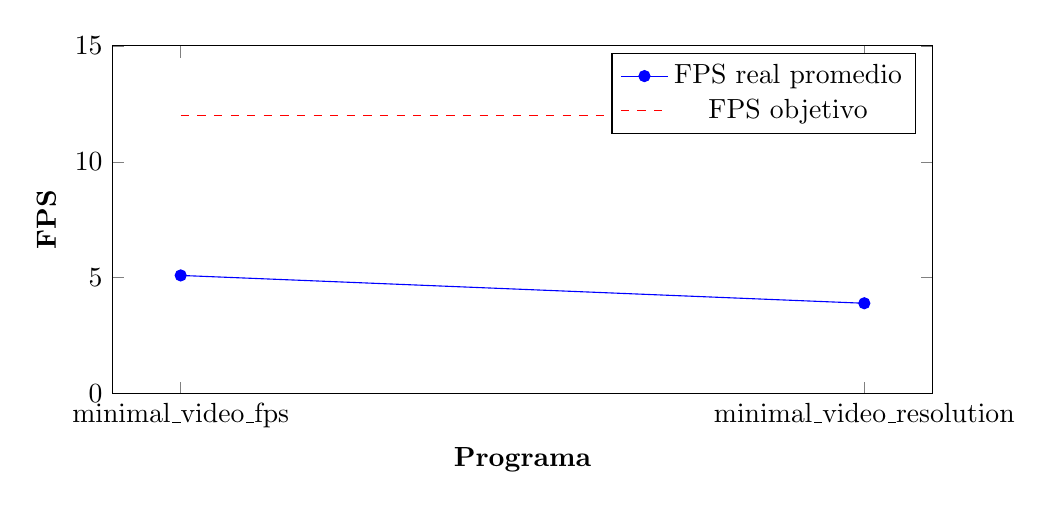
\begin{tikzpicture}
\begin{axis}[
    width=12cm,
    height=6cm,
    xlabel={\textbf{Programa}},
    ylabel={\textbf{FPS}},
    symbolic x coords={minimal\_video\_fps, minimal\_video\_resolution},
    xtick=data,
    ymin=0, 
    ymax=15,
    ]
\addplot[mark=*,blue] coordinates {(minimal\_video\_fps, 5.1) (minimal\_video\_resolution, 3.9)};
\addplot[red,sharp plot,dashed] coordinates {(minimal\_video\_fps, 12) (minimal\_video\_resolution, 12)};
\legend{FPS real promedio, FPS objetivo}
\end{axis}
\end{tikzpicture}
\caption{Comparación de FPS entre los dos programas con pérdida de paquetes del 5\%}
\label{fig:comparacionfps_5pct}
\end{figure}

También se muestran las tasas de transmisión y recepción de datos en los siguientes gráficos:
\begin{figure}[H]
\centering
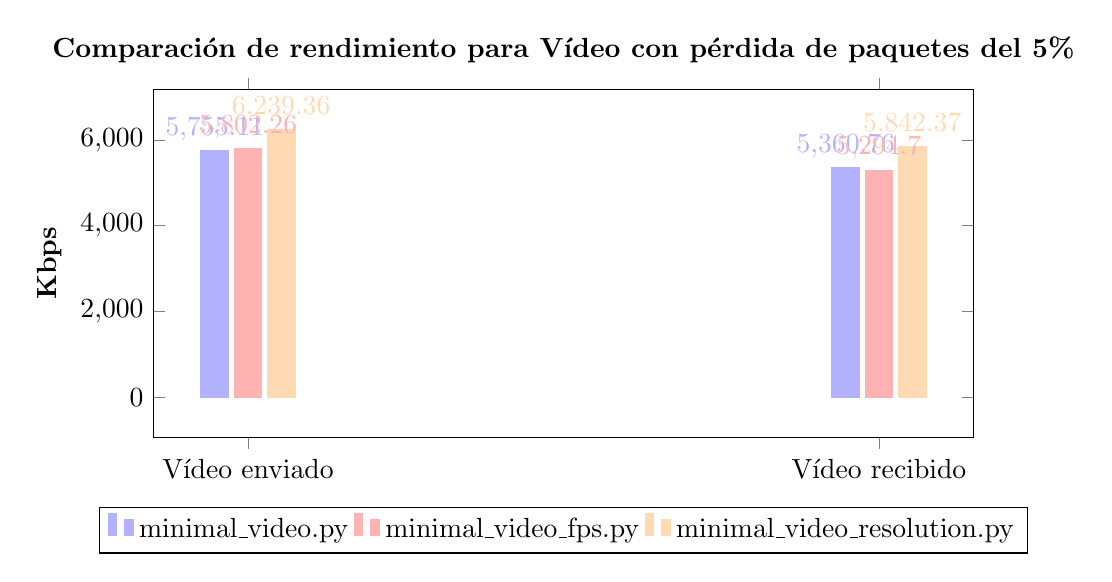
\begin{tikzpicture}
\begin{axis}[
    width=12cm,
    height=6cm,
    ybar,
    enlargelimits=0.15,
    ylabel={\textbf{Kbps}},
    title={\textbf{Comparación de rendimiento para Vídeo con pérdida de paquetes del 5\%}},
    symbolic x coords={Vídeo enviado, Vídeo recibido},
    xtick=data,
    nodes near coords,
    nodes near coords align={vertical},
    ymin=0,
    legend style={at={(0.5,-0.2)}, anchor=north, legend columns=3},
    ]
\addplot[blue!30,fill=blue!30] coordinates {(Vídeo enviado, 5755.11) (Vídeo recibido, 5360.76)};
\addplot[red!30,fill=red!30] coordinates {(Vídeo enviado, 5802.26) (Vídeo recibido, 5294.70)};
\addplot[orange!30,fill=orange!30] coordinates {(Vídeo enviado, 6239.36) (Vídeo recibido, 5842.37)};
\legend{minimal\_video.py, minimal\_video\_fps.py, minimal\_video\_resolution.py}
\end{axis}
\end{tikzpicture}

\vspace{0.5cm} % Espacio entre gráficas

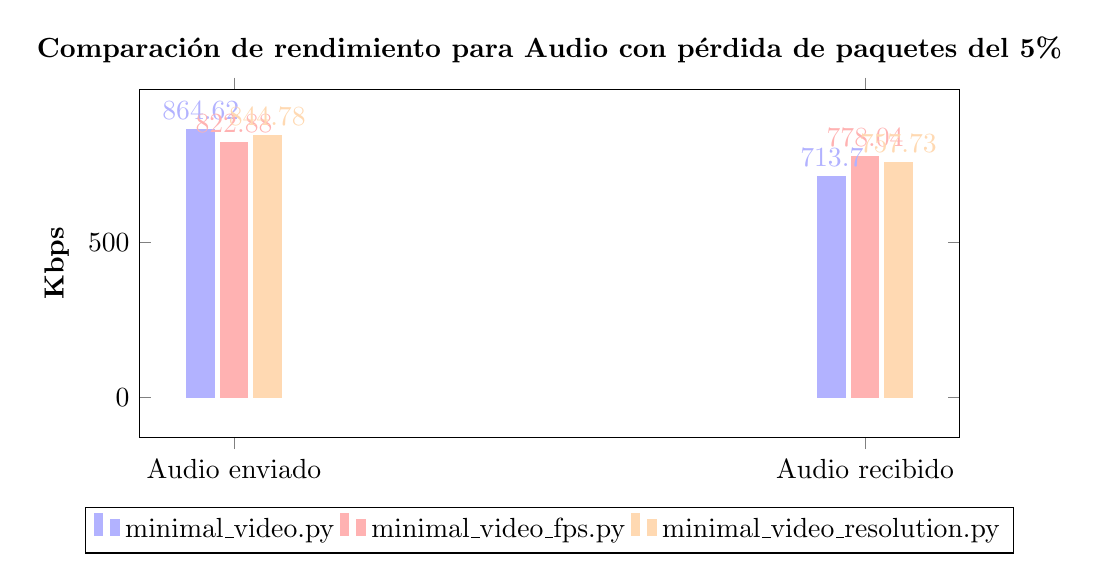
\begin{tikzpicture}
\begin{axis}[
    width=12cm,
    height=6cm,
    ybar,
    enlargelimits=0.15,
    ylabel={\textbf{Kbps}},
    title={\textbf{Comparación de rendimiento para Audio con pérdida de paquetes del 5\%}},
    symbolic x coords={Audio enviado, Audio recibido},
    xtick=data,
    nodes near coords,
    nodes near coords align={vertical},
    ymin=0,
    legend style={at={(0.5,-0.2)}, anchor=north, legend columns=3},
    ]
\addplot[blue!30,fill=blue!30] coordinates {(Audio enviado, 864.62) (Audio recibido, 713.70)};
\addplot[red!30,fill=red!30] coordinates {(Audio enviado, 822.88) (Audio recibido, 778.04)};
\addplot[orange!30,fill=orange!30] coordinates {(Audio enviado, 844.78) (Audio recibido, 757.73)};
\legend{minimal\_video.py, minimal\_video\_fps.py, minimal\_video\_resolution.py}
\end{axis}
\end{tikzpicture}
\caption{Comparación del rendimiento de los tres programas con pérdida de paquetes del 5\%}
\label{fig:comparacion5pct}
\end{figure}

\textbf{Conclusiones para pérdida de paquetes del 5\%:}

La prueba con una pérdida de paquetes moderada del 5\% muestra aspectos interesantes sobre los tres módulos:

\begin{itemize}
    \item \textbf{Impacto en la recepción:} Los tres módulos muestran tasas de recepción bastante aceptables (entre 82.5\% y 94.6\%), con variaciones notables entre audio y vídeo que sugieren diferentes mecanismos de priorización.
    
    \item \textbf{Degradación significativa de FPS:} A pesar de las buenas tasas de recepción, la eficiencia de FPS se ve gravemente afectada en los tres módulos, especialmente en \texttt{minimal\_video\_resolution.py} con solo un 32.2\% de eficiencia.
    
    \item \textbf{Comportamiento irregular entre ciclos:} El análisis por ciclos muestra una variabilidad grande, con algunos períodos de transmisión casi perfecta y otros con pérdidas significativas, creando una experiencia de usuario inconsistente.
    
    \item \textbf{Aumento del uso de CPU:} Todos los módulos muestran picos elevados de uso de CPU (llegando al 85-95\% en algunos ciclos), reflejando el trabajo adicional necesario para gestionar las pérdidas y mantener la comunicación.
\end{itemize}

Estos resultados indican que incluso una pérdida de paquetes moderada del 5\% puede tener un impacto considerable en la calidad de la comunicación en tiempo real. Aunque no impide completamente la comunicación, afecta notablemente la fluidez visual y, en menor medida, la calidad del audio.

\newpage

\begin{itemize}
  \item \textbf{Prueba de pérdida de paquetes del 25\%:}
\end{itemize}

Ahora analizamos el comportamiento de los tres módulos bajo un escenario de pérdida de paquetes del 25\%, que representa una situación de red severamente degradada como podría ocurrir en conexiones inalámbricas con alta interferencia, redes muy congestionadas o condiciones de conectividad extremadamente adversas.

\vspace{\baselineskip}

\textbf{- Análisis de \texttt{minimal\_video.py} con 25\% de pérdida de paquetes:}
\vspace{\baselineskip}

El impacto de una pérdida de paquetes del 25\% en \texttt{minimal\_video.py} es dramático. Las estadísticas globales revelan que el módulo envía audio a 1005.18 kbps pero recibe solo 359.70 kbps (64\% de pérdida), mientras que para vídeo envía 3357.26 kbps y recibe 2514.37 kbps (25\% de pérdida). La disparidad entre el porcentaje teórico de pérdida (25\%) y la pérdida real observada en el audio (64\%) sugiere un efecto cascada donde la pérdida de ciertos paquetes clave compromete secuencias enteras de comunicación.

El análisis por ciclos muestra un comportamiento extremadamente errático. Por ejemplo, en el ciclo 12, de 37 mensajes de audio enviados solo se recibieron 12 (32\%), y en el ciclo 9, de 30 mensajes solo llegaron 5 (17\%). Esta inconsistencia provoca una experiencia fragmentada con constantes interrupciones tanto en el audio como en el vídeo. La comunicación se vuelve prácticamente ininteligible, con largos períodos de silencio y fotogramas congelados seguidos por actualizaciones breves y a menudo distorsionadas.

\vspace{\baselineskip}

\textbf{Análisis de \texttt{minimal\_video\_fps.py} con 25\% de pérdida de paquetes:}
\vspace{\baselineskip}

Este módulo sufre igualmente un impacto severo bajo una pérdida de paquetes tan elevada. Las estadísticas globales muestran una transmisión de audio de 1101.04 kbps (recibiendo 411.82 kbps, 63\% de pérdida) y de vídeo de 4089.65 kbps (recibiendo 3027.28 kbps, 26\% de pérdida). Estos porcentajes revelan nuevamente un impacto desproporcionado en el audio comparado con el vídeo.

Las ``Estadísticas de FPS'' muestran un dato crítico: el módulo solo alcanza 2.9 FPS reales frente al objetivo de 12 FPS, resultando en una eficiencia del 23.8\%. Esta tasa de fotogramas es extremadamente baja para una comunicación visual efectiva. El algoritmo de control de FPS, al detectar las pérdidas masivas, reduce drásticamente la frecuencia de envío, priorizando la integridad de los pocos fotogramas que logran transmitirse sobre la fluidez global. El resultado es una experiencia visual severamente degradada, con actualizaciones de imagen tan esporádicas que dificultan la percepción de movimiento natural.

\vspace{\baselineskip}

\textbf{Análisis de \texttt{minimal\_video\_resolution.py} con 25\% de pérdida de paquetes:}
\vspace{\baselineskip}

Este módulo, que combina control de FPS con resolución adaptada, muestra el peor rendimiento bajo condiciones de pérdida del 25\%. Los datos globales indican una transmisión de audio de 1109.15 kbps (recibiendo 457.32 kbps, 59\% de pérdida) y de vídeo de 3820.40 kbps (recibiendo 2859.69 kbps, 25\% de pérdida).

Las ``Estadísticas de FPS'' revelan un resultado crítico: apenas 1.8 FPS reales frente al objetivo de 12 FPS, con una eficiencia catastrófica del 15.3\%. En términos prácticos, esto significa aproximadamente una actualización de imagen cada 0.55 segundos, insuficiente para cualquier comunicación visual interactiva. El ``Tiempo de reescalado promedio`` aumenta a 7.67 ms, con un impacto en rendimiento del 9.2\%, valores superiores a los observados en condiciones menos adversas. Este aumento refleja la carga adicional que supone intentar procesar y reescalar fotogramas fragmentados o corruptos debido a la pérdida de paquetes.

\vspace{\baselineskip}

Además, a continuación se muestra la eficiencia de FPS en minimal\_video\_fps y minimal\_video\_resolution en el siguiente gráfico:
\begin{figure}[H]
\centering
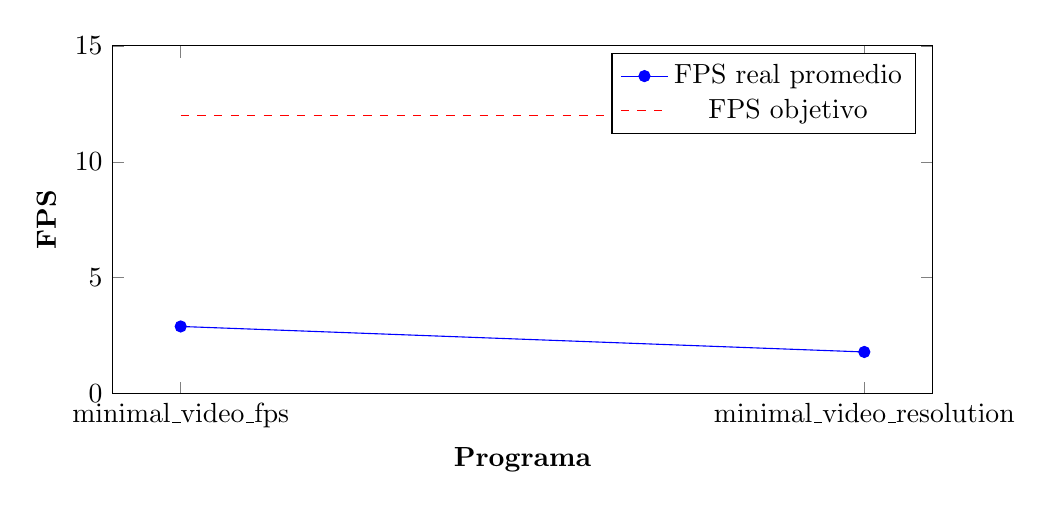
\begin{tikzpicture}
\begin{axis}[
    width=12cm,
    height=6cm,
    xlabel={\textbf{Programa}},
    ylabel={\textbf{FPS}},
    symbolic x coords={minimal\_video\_fps, minimal\_video\_resolution},
    xtick=data,
    ymin=0, 
    ymax=15,
    ]
\addplot[mark=*,blue] coordinates {(minimal\_video\_fps, 2.9) (minimal\_video\_resolution, 1.8)};
\addplot[red,sharp plot,dashed] coordinates {(minimal\_video\_fps, 12) (minimal\_video\_resolution, 12)};
\legend{FPS real promedio, FPS objetivo}
\end{axis}
\end{tikzpicture}
\caption{Comparación de FPS entre los dos programas con pérdida de paquetes del 25\%}
\label{fig:comparacionfps_25pct}
\end{figure}

También se muestran las tasas de transmisión y recepción de datos en los siguientes gráficos:
\begin{figure}[H]
\centering
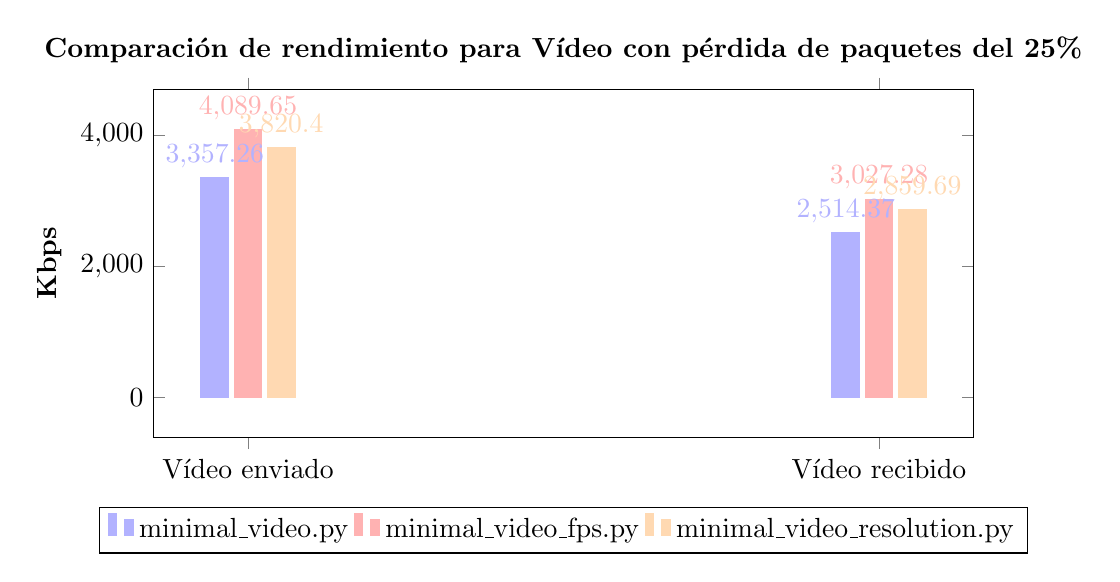
\begin{tikzpicture}
\begin{axis}[
    width=12cm,
    height=6cm,
    ybar,
    enlargelimits=0.15,
    ylabel={\textbf{Kbps}},
    title={\textbf{Comparación de rendimiento para Vídeo con pérdida de paquetes del 25\%}},
    symbolic x coords={Vídeo enviado, Vídeo recibido},
    xtick=data,
    nodes near coords,
    nodes near coords align={vertical},
    ymin=0,
    legend style={at={(0.5,-0.2)}, anchor=north, legend columns=3},
    ]
\addplot[blue!30,fill=blue!30] coordinates {(Vídeo enviado, 3357.26) (Vídeo recibido, 2514.37)};
\addplot[red!30,fill=red!30] coordinates {(Vídeo enviado, 4089.65) (Vídeo recibido, 3027.28)};
\addplot[orange!30,fill=orange!30] coordinates {(Vídeo enviado, 3820.40) (Vídeo recibido, 2859.69)};
\legend{minimal\_video.py, minimal\_video\_fps.py, minimal\_video\_resolution.py}
\end{axis}
\end{tikzpicture}

\vspace{0.1cm} % Espacio entre gráficas

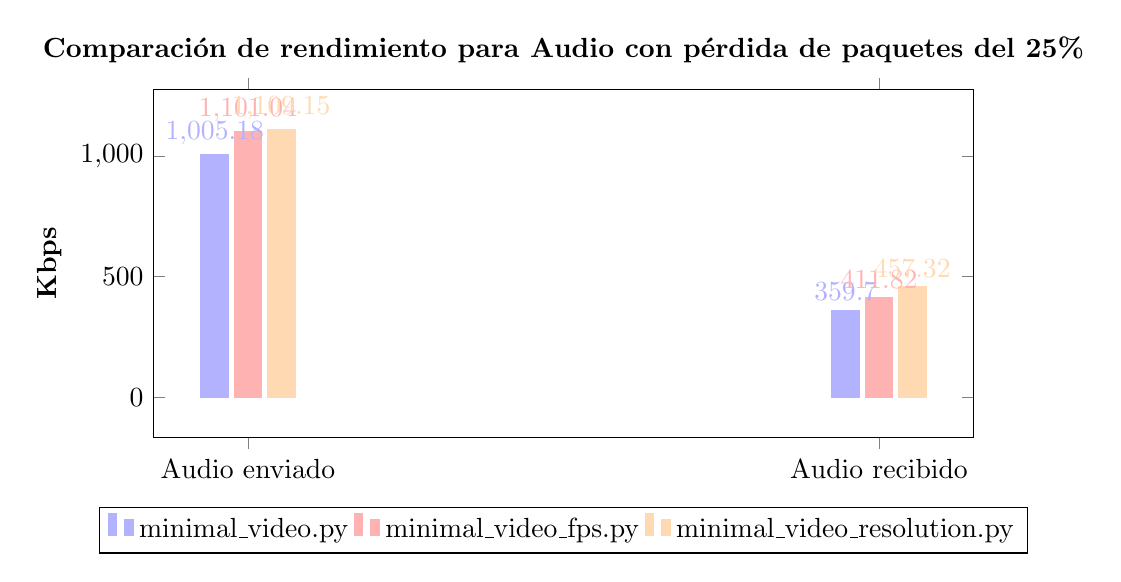
\begin{tikzpicture}
\begin{axis}[
    width=12cm,
    height=6cm,
    ybar,
    enlargelimits=0.15,
    ylabel={\textbf{Kbps}},
    title={\textbf{Comparación de rendimiento para Audio con pérdida de paquetes del 25\%}},
    symbolic x coords={Audio enviado, Audio recibido},
    xtick=data,
    nodes near coords,
    nodes near coords align={vertical},
    ymin=0,
    legend style={at={(0.5,-0.2)}, anchor=north, legend columns=3},
    ]
\addplot[blue!30,fill=blue!30] coordinates {(Audio enviado, 1005.18) (Audio recibido, 359.70)};
\addplot[red!30,fill=red!30] coordinates {(Audio enviado, 1101.04) (Audio recibido, 411.82)};
\addplot[orange!30,fill=orange!30] coordinates {(Audio enviado, 1109.15) (Audio recibido, 457.32)};
\legend{minimal\_video.py, minimal\_video\_fps.py, minimal\_video\_resolution.py}
\end{axis}
\end{tikzpicture}
\caption{Comparación del rendimiento de los tres programas con pérdida de paquetes del 25\%}
\label{fig:comparacion25pct}
\end{figure}

\textbf{Conclusiones para pérdida de paquetes del 25\%:}

Una pérdida de paquetes del 25\% representa un escenario catastrófico para aplicaciones de videoconferencia, revelando limitaciones fundamentales en los tres módulos:

\begin{itemize}
    \item \textbf{Pérdida desproporcionada en audio:} Los tres módulos muestran pérdidas de audio cercanas al 60\%, muy superiores al 25\% teórico, lo que sugiere un efecto multiplicador donde la pérdida de ciertos paquetes críticos compromete secuencias enteras de comunicación.
    
    \item \textbf{Tasas de FPS críticas:} Los valores de 1.8-2.9 FPS están muy por debajo del umbral mínimo para una comunicación visual fluida (generalmente considerado en torno a 10-15 FPS), haciendo que la videoconferencia sea prácticamente inviable.
    
    \item \textbf{Comportamiento errático:} El análisis por ciclos muestra variaciones extremas en la recepción, con momentos donde apenas llega el 10-15\% de los mensajes, creando una experiencia fragmentada e inconsistente.
    
    \item \textbf{Mayor consumo de recursos:} A pesar de procesar menos datos efectivos debido a las pérdidas, se observa un incremento en el uso de CPU, reflejando el esfuerzo adicional para detectar, gestionar y recuperarse de las pérdidas masivas.
    
    \item \textbf{Degradación proporcional a la complejidad:} El módulo más sofisticado (\texttt{minimal\_video\_resolution.py}) muestra el peor rendimiento (15.3\% de eficiencia), evidenciando que las características avanzadas son más vulnerables ante condiciones de red severas.
\end{itemize}

Estos resultados demuestran que una pérdida de paquetes del 25\% sobrepasa ampliamente la capacidad de adaptación de los tres módulos, resultando en una comunicación que difícilmente puede considerarse funcional. En entornos con pérdidas tan elevadas, sería necesario implementar técnicas avanzadas como codificación redundante, transmisión prioritaria de datos críticos o incluso cambiar a modos menos exigentes (por ejemplo, desactivar el vídeo y mantener solo audio) para preservar algún nivel de comunicación efectiva.

\newpage

\begin{itemize}
  \item \textbf{Prueba de pérdida de paquetes del 50\%:}
\end{itemize}

Finalizamos nuestro estudio analizando el comportamiento de los tres módulos bajo un escenario extremo de pérdida de paquetes del 50\%, que representa una situación de red crítica, prácticamente colapsada, como podría ocurrir en conexiones inalámbricas con interferencia severa o redes completamente saturadas.

\vspace{\baselineskip}

\textbf{- Análisis de \texttt{minimal\_video.py} con 50\% de pérdida de paquetes:}
\vspace{\baselineskip}

El impacto de una pérdida de paquetes del 50\% en \texttt{minimal\_video.py} es devastador. Las estadísticas globales muestran que el módulo envía audio a 944.42 kbps pero recibe solo 136.63 kbps (una pérdida catastrófica del 85.5\%), mientras que para vídeo envía 2972.17 kbps y recibe apenas 1376.93 kbps (una pérdida del 53.7\%). Estos valores muestran que el rendimiento real es peor que el teorico ya que se pierden mas del 50\%, especialmente en el audio.
\vspace{\baselineskip}

Muchos ciclos no reciben ningun paquete, mientras que otros muestran una recepción mínima y fragmentada. Por ejemplo, en el ciclo 6 se enviaron 42 mensajes de audio pero se recibió solo 1, y en el ciclo 7, de 40 mensajes solo llegaron 5. Esto hace que la comunicación sea inviable, con largos períodos de silencio total intercalados con algunos datos que si llegan y no permiten mantener ningún tipo de conversación coherente.

\vspace{\baselineskip}

\textbf{Análisis de \texttt{minimal\_video\_fps.py} con 50\% de pérdida de paquetes:}
\vspace{\baselineskip}

Este módulo sufre un colapso casi total. Las estadísticas globales indican una transmisión de audio de 735.36 kbps (recibiendo solo 105.05 kbps, una pérdida del 85.7\%) y de vídeo de 2065.28 kbps (recibiendo 1063.56 kbps, una pérdida del 48.5\%).

Las ``Estadísticas de FPS'' muestran que el módulo apenas alcanza 1.3 FPS reales frente al objetivo de 12 FPS, resultando en una eficiencia catastrófica del 10.7\%. En términos prácticos, esto significa aproximadamente una actualización de imagen cada 0.77 segundos, imposible para cualquier forma de comunicación. El control de FPS trata de mantener una tasa constante y simplemente envía fotogramas completos en muy pocos casos.

\vspace{\baselineskip}

\textbf{Análisis de \texttt{minimal\_video\_resolution.py} con 50\% de pérdida de paquetes:}
\vspace{\baselineskip}

Finalmente, este módulo muestra resultados igualmente catastróficos. Los datos globales revelan una transmisión de audio de 1074.12 kbps (recibiendo 143.22 kbps, una pérdida del 86.7\%) y de vídeo de 2493.55 kbps (recibiendo 1167.06 kbps, una pérdida del 53.2\%).
\vspace{\baselineskip}

Las ``Estadísticas de FPS'' muestran que el módulo apenas alcanza 1.3 FPS reales frente al objetivo de 12 FPS, con una eficiencia del 10.8\%, prácticamente idéntica a la del módulo anterior. Esto es sorprendente teniendo en cuenta que este módulo maneja una resolución mayor (352x288), lo que sugiere que ante pérdidas tan masivas, la limitación principal no es el volumen de datos sino la integridad de la transmisión misma. El ``Tiempo de reescalado promedio`` es de 3.74 ms, con un impacto en rendimiento del 4.5\%, valores que, aunque razonables, resultan irrelevantes cuando la comunicación resulta imposible debido a la pérdida tan grande de paquetes.

\vspace{\baselineskip}

Además, a continuación se muestra la eficiencia de FPS en minimal\_video\_fps y minimal\_video\_resolution en el siguiente gráfico:
\begin{figure}[H]
\centering
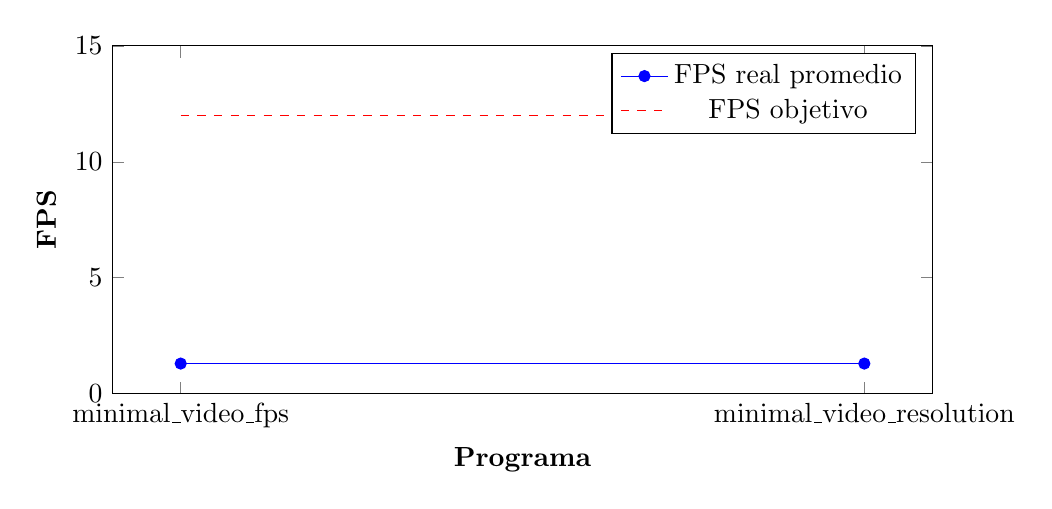
\begin{tikzpicture}
\begin{axis}[
    width=12cm,
    height=6cm,
    xlabel={\textbf{Programa}},
    ylabel={\textbf{FPS}},
    symbolic x coords={minimal\_video\_fps, minimal\_video\_resolution},
    xtick=data,
    ymin=0, 
    ymax=15,
    ]
\addplot[mark=*,blue] coordinates {(minimal\_video\_fps, 1.3) (minimal\_video\_resolution, 1.3)};
\addplot[red,sharp plot,dashed] coordinates {(minimal\_video\_fps, 12) (minimal\_video\_resolution, 12)};
\legend{FPS real promedio, FPS objetivo}
\end{axis}
\end{tikzpicture}
\caption{Comparación de FPS entre los dos programas con pérdida de paquetes del 50\%}
\label{fig:comparacionfps_50pct}
\end{figure}

También se muestran las tasas de transmisión y recepción de datos en los siguientes gráficos:
\begin{figure}[H]
\centering
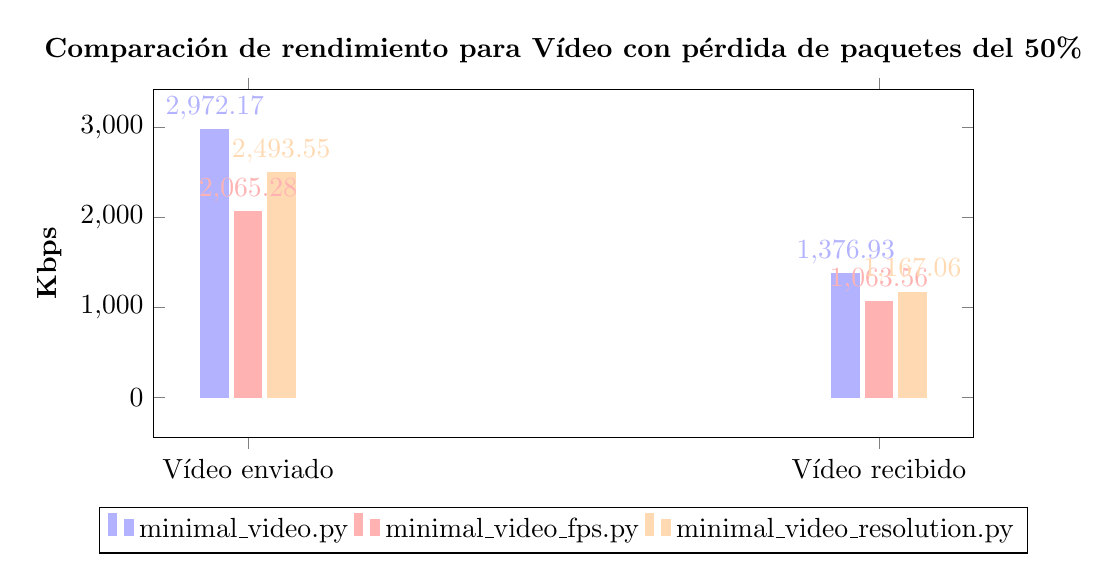
\begin{tikzpicture}
\begin{axis}[
    width=12cm,
    height=6cm,
    ybar,
    enlargelimits=0.15,
    ylabel={\textbf{Kbps}},
    title={\textbf{Comparación de rendimiento para Vídeo con pérdida de paquetes del 50\%}},
    symbolic x coords={Vídeo enviado, Vídeo recibido},
    xtick=data,
    nodes near coords,
    nodes near coords align={vertical},
    ymin=0,
    legend style={at={(0.5,-0.2)}, anchor=north, legend columns=3},
    ]
\addplot[blue!30,fill=blue!30] coordinates {(Vídeo enviado, 2972.17) (Vídeo recibido, 1376.93)};
\addplot[red!30,fill=red!30] coordinates {(Vídeo enviado, 2065.28) (Vídeo recibido, 1063.56)};
\addplot[orange!30,fill=orange!30] coordinates {(Vídeo enviado, 2493.55) (Vídeo recibido, 1167.06)};
\legend{minimal\_video.py, minimal\_video\_fps.py, minimal\_video\_resolution.py}
\end{axis}
\end{tikzpicture}

\vspace{0.8cm} % Espacio entre gráficas

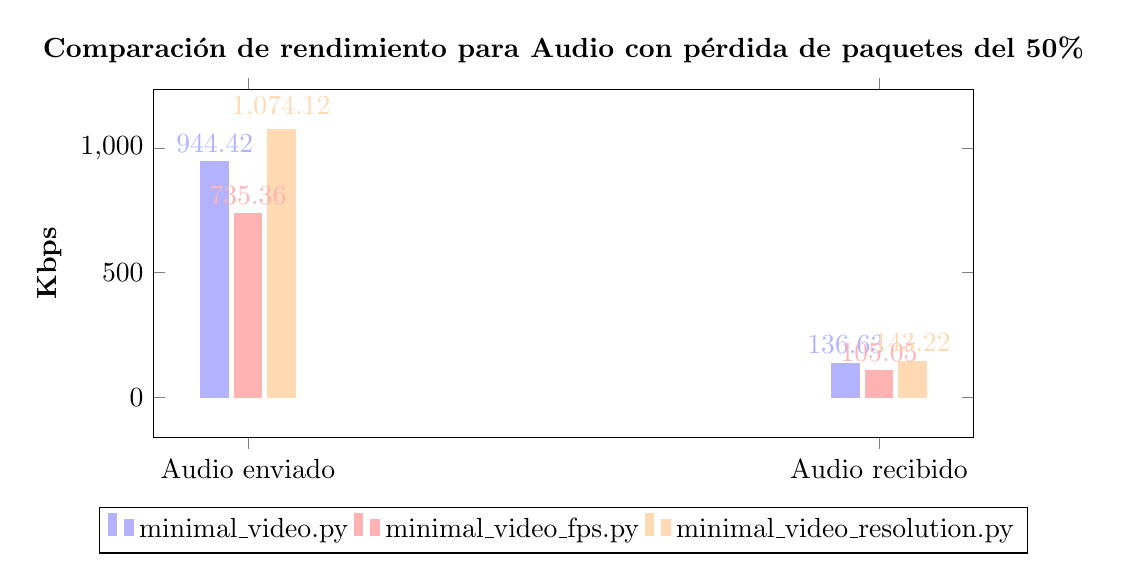
\begin{tikzpicture}
\begin{axis}[
    width=12cm,
    height=6cm,
    ybar,
    enlargelimits=0.15,
    ylabel={\textbf{Kbps}},
    title={\textbf{Comparación de rendimiento para Audio con pérdida de paquetes del 50\%}},
    symbolic x coords={Audio enviado, Audio recibido},
    xtick=data,
    nodes near coords,
    nodes near coords align={vertical},
    ymin=0,
    legend style={at={(0.5,-0.2)}, anchor=north, legend columns=3},
    ]
\addplot[blue!30,fill=blue!30] coordinates {(Audio enviado, 944.42) (Audio recibido, 136.63)};
\addplot[red!30,fill=red!30] coordinates {(Audio enviado, 735.36) (Audio recibido, 105.05)};
\addplot[orange!30,fill=orange!30] coordinates {(Audio enviado, 1074.12) (Audio recibido, 143.22)};
\legend{minimal\_video.py, minimal\_video\_fps.py, minimal\_video\_resolution.py}
\end{axis}
\end{tikzpicture}
\caption{Comparación del rendimiento de los tres programas con pérdida de paquetes del 50\%}
\label{fig:comparacion50pct}
\end{figure}

\textbf{Conclusiones para pérdida de paquetes del 50\%:}

Una pérdida de paquetes del 50\% representa un escenario critico y grave para la comunicación en tiempo real, haciendo que sea inviable la videoconferencia:

\begin{itemize}
    \item \textbf{Pérdida catastrófica en audio:} Los tres módulos muestran pérdidas de audio muy serias: 85-87\% muy superiores al 50\% teórico, provocando que la comunicación sea prácticamente imposible, con apenas fragmentos aislados de sonido perceptibles.
    
    \item \textbf{FPS críticos:} Los valores de 1.0-1.3 FPS están muy por debajo del umbral mínimo para percibir movimiento fluido (generalmente considerado en torno a 10-12 FPS).
    
    \item \textbf{Reducción drástica de ancho de banda utilizado:} Los tres módulos envían datos a tasas muy inferiores a las observadas en escenarios mejores (2-3 Mbps frente a 7-10 Mbps), reflejando cómo los mecanismos de control de congestión detectan el colapso y reducen drásticamente las tasas de transmisión.
    
    \item \textbf{Uso errático de recursos:} El análisis muestra un patrón de uso de CPU extremadamente irregular, con períodos de bajo uso cuando el sistema espera, alternando con picos cuando intenta procesar los pocos paquetes que son recibidos.

\end{itemize}

Estos resultados demuestran que una pérdida de paquetes del 50\% representa un umbral crítico más allá del cual la comunicación audiovisual en tiempo real es fundamentalmente imposible, independientemente de las técnicas empleadas.